
% ----------------------------------------------------------------------
%                   LATEX TEMPLATE FOR PhD THESIS
% ----------------------------------------------------------------------

% based on Harish Bhanderi's PhD/MPhil template, then Uni Cambridge
% http://www-h.eng.cam.ac.uk/help/tpl/textprocessing/ThesisStyle/
% corrected and extended in 2007 by Jakob Suckale, then MPI-CBG PhD programme
% and made available through OpenWetWare.org - the free biology wiki


%: Style file for Latex
% Most style definitions are in the external file PhDthesisPSnPDF.
% In this template package, it can be found in ./Latex/Classes/
\documentclass[twoside,11pt]{Latex/Classes/PhDthesisPSnPDF}


%: Macro file for Latex
% Macros help you summarise frequently repeated Latex commands.
% Here, they are placed in an external file /Latex/Macros/MacroFile1.tex
% An macro that you may use frequently is the figuremacro (see introduction.tex)
% % This file contains macros that can be called up from connected TeX files
% It helps to summarise repeated code, e.g. figure insertion (see below).

% insert a centered figure with caption and description
% parameters 1:filename, 2:title, 3:description and label
\newcommand{\figuremacro}[3]{
	\begin{figure}[htbp]
		\centering
		\includegraphics[width=1\textwidth]{#1}
		\caption[#2]{\textbf{#2} - #3}
		\label{#1}
	\end{figure}
}

% insert a centered figure with caption and description AND WIDTH
% parameters 1:filename, 2:title, 3:description and label, 4: textwidth
% textwidth 1 means as text, 0.5 means half the width of the text
\newcommand{\figuremacroW}[4]{
	\begin{figure}[htbp]
		\centering
		\includegraphics[width=#4\textwidth]{#1}
		\caption[#2]{\textbf{#2} - #3}
		\label{#1}
	\end{figure}
}

% inserts a figure with wrapped around text; only suitable for NARROW figs
% o is for outside on a double paged document; others: l, r, i(inside)
% text and figure will each be half of the document width
% note: long captions often crash with adjacent content; take care
% in general: above 2 macro produce more reliable layout
\newcommand{\figuremacroN}[3]{
	\begin{wrapfigure}{o}{0.5\textwidth}
		\centering
		\includegraphics[width=0.48\textwidth]{#1}
		\caption[#2]{{\small\textbf{#2} - #3}}
		\label{#1}
	\end{wrapfigure}
}

% predefined commands by Harish
\newcommand{\PdfPsText}[2]{
  \ifpdf
     #1
  \else
     #2
  \fi
}

\newcommand{\IncludeGraphicsH}[3]{
  \PdfPsText{\includegraphics[height=#2]{#1}}{\includegraphics[bb = #3, height=#2]{#1}}
}

\newcommand{\IncludeGraphicsW}[3]{
  \PdfPsText{\includegraphics[width=#2]{#1}}{\includegraphics[bb = #3, width=#2]{#1}}
}

\newcommand{\InsertFig}[3]{
  \begin{figure}[!htbp]
    \begin{center}
      \leavevmode
      #1
      \caption{#2}
      \label{#3}
    \end{center}
  \end{figure}
}


%%% Local Variables: 
%%% mode: latex
%%% TeX-master: "~/Documents/LaTeX/CUEDThesisPSnPDF/thesis"
%%% End: 


\usepackage[T1]{fontenc}
\usepackage{array}
\usepackage{pdfpages}
\usepackage{amsmath}
\usepackage{silence}
\WarningFilter{latex}{Text page 39 contains only floats}

% \usepackage{graphics}
% or use the graphicx package for more complicated commands
% \usepackage{graphicx}
\usepackage{pifont} % used for \todo symbol
\newcommand{\todo}[1]{\textcolor{blue}{#1}}

%: ----------------------------------------------------------------------
%:                  TITLE PAGE: name, degree,..
% ----------------------------------------------------------------------
\usepackage{graphicx}
      \textwidth 15cm
      \textheight 22cm
      \parindent 10pt
      \oddsidemargin 0.85cm
      \evensidemargin 0.37cm

% \captionsetup{compatibility=false}
% \usepackage{subcaption}
\usepackage{subfig}
\usepackage{caption}
% \usepackage{listings}

\begin{document}

\thispagestyle{empty}

\begin{center}

Vrije Universiteit Amsterdam \hspace*{2cm} Universiteit van Amsterdam

\vspace{1mm}

\hspace*{-7.5cm}
\includegraphics[height=25mm]{0_frontmatter/figures/vu-griffioen.pdf}

\vspace*{-2cm}\hspace*{7.5cm}
\includegraphics[height=15mm]{0_frontmatter/figures/uva_logo.jpg}

\vspace{2cm}

{\Large Master Thesis}

\vspace*{1.5cm}

\rule{.9\linewidth}{.6pt}\\[0.4cm]
{\huge \bfseries Deep Learning for Neutrino Particle Detection using PointNet \par}\vspace{0.4cm}
\rule{.9\linewidth}{.6pt}\\[1.5cm]

\vspace*{2mm}

{\Large
\begin{tabular}{l}
{\bf Author:} Shruti Rao (2636454)
\end{tabular}
}

\vspace*{2cm}

\begin{tabular}{ll}
{\it 1st supervisor:}   & Dr. Adam Belloum \\
{\it 2nd supervisor:} & Dr. Ben van Werkhoven (Netherlands eScience Center) \\
{\it 2nd reader:}    & Dr. Ronald Bruijn
\end{tabular}

\vspace*{2.5cm}

\textit{A thesis submitted in fulfilment of the requirements for\\ the joint UvA-VU Master of Science degree in Computer Science}

\vspace*{1.8cm}

\today\\[4cm] 

\end{center}

\newpage


% ----------------------------------------------------------------------
       
% turn of those nasty overfull and underfull hboxes
\hbadness=10000
\hfuzz=50pt


%: --------------------------------------------------------------
%:                  FRONT MATTER: dedications, abstract,..
% --------------------------------------------------------------


%\language{english}


% sets line spacing
\renewcommand\baselinestretch{1.2}
\baselineskip=18pt plus1pt


%: ----------------------- generate cover page ------------------------

% \begin{center}
% \textit{``I am the master of my fate, I am the captain of my soul'' \\ from {\em Invictus}, by William Ernest Henley}
% \end{center}

%: ----------------------- cover page back side ------------------------
% Your research institution may require reviewer names, etc.
% This cover back side is required by Dresden Med Fac; uncomment if needed.

\newpage
%\vspace{10mm}
%1. First Reader: Name Surname
%
%\vspace{10mm}
%2. Daily Supervisor: Name Surname
%
%\vspace{10mm}
%3. Second Reader: Name Surname
%
%\vspace{10mm}
%4. Industrial Supervisor: Name Surname
%
%\vspace{20mm}
%Day of the defense:

%\vspace{20mm}
%\hspace{70mm}Signature from head of PhD committee:



%: ----------------------- abstract ------------------------

% Your institution may have specific regulations if you need an abstract and where it is to be placed in the document. The default here is just after title.

\begin{abstracts}  

Particle physics involves examination of sub-atomic particles and their interactions. The main challenge in this field often lies in the separation of background noise from event signals. Most neural networks in the field use CNNs for particle classification. But this often leads to loss of information when converting data to images. This thesis examines the application of PointNet - a 3D classification network for KM3NeT neutrino data. The thesis has a two-fold interest. First, it wishes to investigate the role of 3D deep learning in neutrino identification. Next, it wishes to apply the network on KM3NeT data to save neutrino information while discarding background noise. The data is split into three datasets and trained individually. Feature engineering is performed and the resulting point clouds are converted to 3D meshes. A majority voting ensemble technique is used to combine predictions from the three models. The network showed promising results with a 95\% recall for the positive class and perfect precision. The model also demonstrated perfect recall for the noise class. Being the first known work of its kind, results from the thesis indicate PointNet to be a viable methodology for future neutrino research.

{\bf Keywords:} \textit{PointNet}, \textit{neutrino detection}, \textit{classification}, \textit{3D deep learning}, \textit{KM3NeT}
\end{abstracts}




% The original template provides and abstractseparate environment, if your institution requires them to be separate. I think it's easier to print the abstract from the complete thesis by restricting printing to the relevant page.
% \begin{abstractseparate}
%   \begin{abstracts}  

Particle physics involves examination of sub-atomic particles and their interactions. The main challenge in this field often lies in the separation of background noise from event signals. Most neural networks in the field use CNNs for particle classification. But this often leads to loss of information when converting data to images. This thesis examines the application of PointNet - a 3D classification network for KM3NeT neutrino data. The thesis has a two-fold interest. First, it wishes to investigate the role of 3D deep learning in neutrino identification. Next, it wishes to apply the network on KM3NeT data to save neutrino information while discarding background noise. The data is split into three datasets and trained individually. Feature engineering is performed and the resulting point clouds are converted to 3D meshes. A majority voting ensemble technique is used to combine predictions from the three models. The network showed promising results with a 95\% recall for the positive class and perfect precision. The model also demonstrated perfect recall for the noise class. Being the first known work of its kind, results from the thesis indicate PointNet to be a viable methodology for future neutrino research.

{\bf Keywords:} \textit{PointNet}, \textit{neutrino detection}, \textit{classification}, \textit{3D deep learning}, \textit{KM3NeT}
\end{abstracts}



% \end{abstractseparate}


%: ----------------------- tie in front matter ------------------------

\frontmatter
% % Thesis Dedication ---------------------------------------------------

%\begin{dedication} %this creates the heading for the dedication page

%To ...

%\end{dedication}

% ----------------------------------------------------------------------
\begin{acknowledgements}     

I would like to thank Dr. Adam Belloum and Dr. Ben van Werkhoven for introducing me to the project topic and ensuring its finalisation. I would especially like to thank Dr. Belloum for his constant guidance and advice throughout the course of the thesis. Further, I would like to thank Dr. Roel Aaij, Dr. Ronald Bruin and Brían Ó Fearraigh from Nikhef for assisting with the Physics-based technicalities of the topic. Also, I would like to acknowledge Dr. Aaij's assistance with accessing the Viltstift AMD GPUs, that allowed for rapid experimentation. Finally, I would like to thank my co-worker Arumoy Shome for the exchange of ideas and discussions that enriched the thesis.

\end{acknowledgements}

\let\cleardoublepage\clearpage



%: ----------------------- contents ------------------------

\setcounter{secnumdepth}{3} % organisational level that receives a numbers
\setcounter{tocdepth}{3}    % print table of contents for level 3
\tableofcontents            % print the table of contents
% levels are: 0 - chapter, 1 - section, 2 - subsection, 3 - subsection


%: ----------------------- list of figures/tables ------------------------

\listoffigures	% print list of figures
\let\cleardoublepage\clearpage

\listoftables  % print list of tables
\let\cleardoublepage\clearpage

%: ----------------------- glossary ------------------------

% Tie in external source file for definitions: /0_frontmatter/glossary.tex
% Glossary entries can also be defined in the main text. See glossary.tex
% 
%% this file is called up by thesis.tex
% content in this file will be fed into the main document

% Glossary entries are defined with the command \nomenclature{1}{2}
% 1 = Entry name, e.g. abbreviation; 2 = Explanation
% You can place all explanations in this separate file or declare them in the middle of the text. Either way they will be collected in the glossary.

% required to print nomenclature name to page header
%\markboth{\MakeUppercase{\nomname}}{\MakeUppercase{\nomname}}


% ----------------------- contents from here ------------------------


%\nomenclature{LSY}{ehbfuefebbfbjkjkebfjbfbfw} 
%\nomenclature{DEPC}{diethyl-pyro-carbonate; used to remove RNA-degrading enzymes (RNAases) from water and laboratory utensils}
%\nomenclature{DMSO}{dimethyl sulfoxide; organic solvent, readily passes through skin, cryoprotectant in cell culture}
%\nomenclature{EDTA}{Ethylene-diamine-tetraacetic acid; a chelating (two-pronged) molecule used to sequester most divalent (or trivalent) metal ions, such as calcium (Ca$^{2+}$) and magnesium (Mg$^{2+}$), copper (Cu$^{2+}$), or iron (Fe$^{2+}$ / Fe$^{3+}$)}



 

%\begin{multicols}{2} % \begin{multicols}{#columns}[header text][space]
%\begin{footnotesize} % scriptsize(7) < footnotesize(8) < small (9) < normal (10)

%\printnomenclature[1.5cm] % [] = distance between entry and description
%\label{nom} % target name for links to glossary

%\end{footnotesize}
%\end{multicols}

%: --------------------------------------------------------------
%:                  MAIN DOCUMENT SECTION
% --------------------------------------------------------------

% the main text starts here with the introduction, 1st chapter,...
\mainmatter

\renewcommand{\chaptername}{} % uncomment to print only "1" not "Chapter 1"

%: ----------------------- subdocuments ------------------------

% Parts of the thesis are included below. Rename the files as required.
% But take care that the paths match. You can also change the order of appearance by moving the include commands.

\chapter{Introduction}

\ifpdf
    \graphicspath{{1_introduction/figures/PNG/}{1_introduction/figures/PDF/}{1_introduction/figures/}}
\else
    \graphicspath{{1_introduction/figures/EPS/}{1_introduction/figures/}}
\fi

Physics has accounted for many fundamental properties of the universe. Yet, several questions regarding the elementary constituents of matter remain unanswered. For instance, it is well known that when neutron stars collide, they produce supermassive stars or black holes \cite{bekenstein1973black}. However, there is not much information on what the cores of such stars or black holes comprise of. Similarly, it has also been established that majority of the universe is comprised of dark matter, with little indication as to what dark matter really constitutes \cite{halliwell1985origin}. What is however known is that all of these phenomena have one particle in common - the neutrino \cite{bekenstein1973black}. Neutrinos are elusive, weakly interacting particles that were discovered first by Pauli in the 1930s and the only known particle making up dark matter \cite{bilenky2013neutrino, roberts1992birth}. Understanding neutrinos has become increasingly significant for researchers in recent times as it represents much of the unknown universe. Experiments are being conducted to understand the mass of neutrinos, reasons for their oscillation, their ability to change forms, and the role they play in the birth and continuum of the universe \cite{gray2011cosmic}. 

With simultaneous advancement in hardware and computing power, the ability to detect and understand neutrinos has drastically increased \cite{bilenky2013neutrino, roberts1992birth, acciarri2016long, acciarri2017convolutional, albert2020antares, aiello2019sensitivity}. Large particle accelerators are typical in particle physics experiments whereby protons and anti-protons are collided at high speeds to try to recreate neutrino particles. Through this process, petabytes of data are often produced and have to be analysed for signs of tracks, rings, jets and showers associated with neutrino interactions \cite{britton2014deal}. These experiments so far have made use of physics algorithms that have worked well in detecting particles to a certain degree. However, these techniques fall short when it comes to identifying new particles or studying previously unknown behaviour that has not been defined by the algorithm parameters \cite{edelen2016neural}. Traditional algorithms are also unable to keep up with large volumes of rapidly changing, high dimensional data. Thus, reliance on such algorithms have limited the potential for new discoveries \cite{edelen2016neural}.

On the other hand, Neural Networks (NNs) have faced several cycles of hype over the past decade or so. Early attempts at incorporating NNs were often unsuccessful due to limited understanding, large computation hours, hardware limitations, and lack of powerful architectures \cite{ahmed1974discrete}. Early applications that were developed were highly sensitive to errors and data quality \cite{ahmed1974discrete}. Due to these reasons, Neural Networks were not a favoured solution. But, recent advances in computing led to better storage of data, faster execution times and improved error handling. These factors directly contributed to enabling real-time processing of data. Also, since storage of large datasets was now possible, networks could be trained with larger datasets. Additionally, general theoretical research was advanced to address the concept of NNs being a black-box. Advances in computational theory led to development of powerful learning algorithms, optimisation techniques and robust architectures \cite{bottou2010large}. These factors combined led to new interest in application of NNs to complicated problems, including those in particle physics \cite{edelen2016neural}.

\section{Background} 
In order to understand the motivation behind the work done by this thesis and ongoing research, it is essential to understand the fundamental properties of neutrinos. It is also important to examine some significant existing applications of Neural Networks in working detectors. These can help identify scope for improvement for this thesis and for future research.

\subsection{Neutrinos}
% What are neutrinos & how are they produced
Neutrinos are fundamental particles of the universe and quite different in nature from other commonly known particles. They carry no charge, are extremely small in mass and travel through matter undetected \cite{bilenky2013neutrino}. Neutrinos come in three types (flavours) and can change between types and masses \cite{bilenky2013neutrino}. On Earth, neutrinos are produced by nuclear reactors, natural radioactive changes in the atmosphere and particle accelerators. The Sun produces neutrinos via nuclear fission that occurs in its core. They are also generated from the births, deaths and collisions of stars and supernovae explosions \cite{roberts1992birth}. 

% Why are they hard to detect
Detecting neutrinos are extremely hard because they rarely interact. Around a trillion neutrinos pass through the Earth every second yet, approximately only one neutrino reacts with matter on Earth, once a day \cite{abi2018dune, acciarri2016long}.  A neutrino travelling near the nucleus of an atom emits weak bosons (W and Z type) \cite{bahcall1989neutrino}. These in turn react with the nucleus of another atom to produce a multitude of particles, including charged particles which can be detected. However, the probability of the weak bosons hitting a nucleus of another atom is extremely small. This is because weak bosons have a very short lifetime of $1 \times 10^{-27}$ seconds and travel a very short distance of less than $0.001$ of the size of a proton \cite{bahcall1989neutrino, adamson2008study, puccini2018bosons}. These two reasons make it very hard for charged particles to be produced and in turn for neutrinos to be detected. 

% How do you detect neutrinos
\label{sec:intro-detection-of-neutrinos}
There are a few ways of detecting neutrinos, with under-water detectors being most popular. In water, neutrino particles travel undisturbed and may travel faster than light in that medium. They may react with matter particles in water and create a charged \textit{lepton} that produces a light known as \textit{Cherenkov light}. These flashes of light are detected by photomultiplier (PMT) tubes that can infer direction, energy and flavour of the neutrino \cite{adamson2008study}. \textit{Super Kamiokande} is a water based detector that uses \textit{Cherenkov light} to detect neutrinos \cite{tanaka2020search}. \textit{IceCube} is another experiment located in the South Pole that uses a cubic kilometre of ice embedded with PMT tubes to detect neutrino events \cite{albert2020antares}. \textit{MiniBooNE} detector uses pure mineral oil that allows low energy muons and protons, invisible in water, to be detected \cite{aguilar2017dark}.

% Why are they important
Neutrinos are important because understanding their origin can help resolve many physics unknowns. Neutrinos could be used to probe and examine matter that present radiation cannot pass through. Since they travel through space practically unaffected, physicists believe that neutrinos can help learn about galactic cores and supernovae. 


\subsection{Neural Networks in Neutrino Physics}
Neural Networks were first acknowledged in physics around 1988, in the field of particle physics \cite{denby1999neural}. Particle physics comprises the study of the fundamental building blocks of nature. It largely involves low-level pattern recognition and physics process determination. According to Denby (1999), low-level pattern recognition tasks include finding tracks made by particles and process determination encompasses obtaining properties such as spatial topology and energy emissions of particles. Studies of such processes require work to be done either in real-time or offline. Denby (1999) described particle physics processes to be characterised by large magnitudes of background noise with small, rarer occurrences of real events at any given point in time \cite{denby1999neural}. 

Denby (1999) found Neural Networks in particle physics that have been used in both real-time and offline applications. Overall, NNs have had challenges being recognised as a statistical tool within the community of particle research. The main challenge in particle physics lies in the fact that such experiments often have to deal with new and unknown phenomena. NNs in such instances have to be developed based on unknown, and guessed parameters. Models trained on such parameters then further reflect these unknowns and inaccuracies \cite{denby1999neural}. 

Despite these accepted fallacies, there are a few large-scale detector experiments that have incorporated Neural Networks. \textit{Fermilab} has a muon trigger that applies low-level pattern recognition techniques \cite{adamson2008study}. \textit{Fermilab} also uses NNs to analyse proton-anti-proton collisions and measures top-quarks and lepto-quarks \cite{adamson2008study}. The \textit{Hera} accelerator has a prototype experiment that studies momentum from colliding particles \cite{voss1994electron} and a secondary experiment called \textit{ZEUS} that uses a form of feedforward network to identify deeply inelastic neutral current events \cite{abramowicz1995neural}. The \textit{CMS} experiment at the Large Hadron Collider (LHC) uses a neural network based trigger to identify electrons from protons \cite{chatrchyan2010performance}. 

\section{KM3NeT}
\label{sec:intro-km3net}
KM3NeT (Cubic Kilometre Neutrino Telescope) is a next generation neutrino telescope project, currently being constructed under the Mediterranean Sea \footnote{https://www.km3net.org/}. The research unit comprises two main telescopes - the ARCA (Astroparticle Research with Cosmics in the Abyss) and the ORCA (Oscillation Research with Cosmics in the Abyss) \cite{km3net_2017}. The ARCA telescope is to be used for extraterrestrial neutrino particles originating from the likes of supernovae or colliding stars \cite{km3net_2017}. The ORCA telescope will be used to examine neutrinos travelling through the Earth's atmosphere \cite{km3net_2017}. KM3NeT is another example of the underwater detectors discussed in Section \ref{sec:intro-detection-of-neutrinos}, and relies on optical sensors to detect \textit{Cherenkov light} \cite{km3net_2017}. These highly sensitive photomultiplier tubes also acquire a significant amount of noise generated by other background factors, mainly Potassium-40 decay. The detector therefore records all photon particles as hits and solutions are in place to try and isolate relevant hits from noise hits. 

\subsection{Event Triggers}
\label{sec:intro-trigger}
Data acquisition for the offshore KM3NeT detectors is based on a preset threshold, whereby all analogue signals that exceed the threshold are sent to shore. This is known as the level-zero (L0) filter. Next, event based level-one (L1) trigger is employed to filter out relevant events. Specifically, the occurrence of two or more L0 hits within a certain time and spatial distance are considered significant for L1 \cite{km3net_2017}. 

\subsection{GPU Pipeline}
A separate GPU-based data processing pipeline was proposed as a viable solution to the event-based triggers by Karas (2019). The pipeline comprises of three components. The first component of the pipeline implements hits correlation based on closeness of hits in time and space, given a threshold. The second phase of the pipeline uses the correlation from the previous component to cluster related hits together. The final phase of the pipeline then classifies communities into significant and insignificant ones, based on the presence of neutrino events \cite{karas_2019}.
 
\section{Research Questions}
\label{sec:intro-research-questions}
Typically, particle physics research relies on building physics-derived algorithms to detect neutrinos. Previously described event triggers and the GPU pipeline for the KM3NeT are two such examples (Sec: \ref{sec:intro-km3net}). While these algorithms are physics driven, they may fall short when trying to capture complex information from imbalanced, skewed data. This could be due to three main reasons:
\begin{enumerate}
    \item Often, physics algorithms make use of theoretical parameters and criterion that may not be optimised across varied datasets.
    \item Algorithms designed to work on smaller, lower dimensional data may not be able to model increasingly higher dimensional data without suffering from information loss.
    \item Several physics algorithms are highly customised and specific to the problem or data at hand, lacking in ability to be generalised \cite{denby1999neural}. 
\end{enumerate}

Examination of literature on the topic has shown popularity of Convolutional Neural Networks (CNNs) for neutrino research. This also faces drawbacks, mainly from information loss and high compute times. Converting detector data to images and learning to detect neutrinos from them will lead to loss of information that may have been useful. It is imperative to understand if existing methodologies such as physics-based triggers and CNNs can be replaced by new models and data representations. 
Point clouds are the simplest representation of 3D geometric objects and could be one such means to represent neutrino data in a novel manner. PointNet, a point cloud specific architecture could be used to train on such data. The following research questions were formulated to address the feasibility of using PointNet for neutrino identification amidst background noise:

\begin{description}
    \item[\textbf{RQ1.0}] \textit{Can PointNet, a geometric neural network architecture be trained to identify timeslices that contain neutrino event hits from timeslices that contain only background noise?} \\
    The KM3NeT detector gathers large volumes of data in real-time and sends it onshore in chunks of time (timeslices) \cite{km3net_2017}. It would be computationally infeasible to store all of this data when most of it may be irrelevant to research. Therefore, an effective method is required to identify timeslices that contain neutrino hits so that only they may be saved and the rest gets discarded. 
    
    \item[\textbf{RQ1.1}] \textit{Can PointNet achieve a Recall score of greater than 0.9 for identifying timeslices with event hits?} \\
    KM3NeT stakeholders defined 90\% recall score for the model, which is the ability of the algorithm to learn from the data. To provide valuable contributions, PointNet would have to score 90\% or higher for Recall.
    
    \item[\textbf{RQ2.0}] \textit{Can the KM3NeT dataset be effectively represented using 3D meshes?} \\
    PointNet typically learns from 3D meshes while the KM3NeT data comprises of \texttt{x, y, z} coordinates, \texttt{time} and metadata. If these attributes can be modelled to form a surface-based 3D mesh, it could serve as a suitable training data for PointNet as a 3D mesh stores more information about geometry than just 3D coordinates.
    
    \item[\textbf{RQ2.1}] \textit{Which meshing algorithm would be most suitable for representing the data?}  \\
    The dataset is challenging as it does not contain any discerning features. Event hits are characterised by how close they occur in time and space, compared to noise hits. Yet this closeness is not very prominent. Conversion of points to 3D meshes will result transformation of data. It is essential to ensure that the transformation is such that much of the valuable information regarding event hits is maintained, if not enhanced. An ideal algorithm would allow minute differences amongst event hits to stand out more than noise.
  
    \item[\textbf{RQ3.0}] \textit{Can PointNet be extended to obtain energy properties from neutrino events?} \\
    Inferring energy from neutrino events can help identify and study the processes that formed it. PointNet is a classification specific architecture but as it learns from both local and global structure of point clouds, it may be able solve other tasks related to point cloud recognition including regression \cite{qi2017pointnet}.
\end{description}


\section{Research Outcomes}
With research in particle physics turning to AI, a rigorous assessment of state-of-the-art networks is required to identify those best for the task at hand. This thesis aims to provide an in-depth investigation of one such state-of-the-art neural network - PointNet.  This thesis contributes to the current state of knowledge by assessing the potential of 3D Neural Networks for research in neutrinos. In order to achieve this goal, an ensemble of data from the KM3NeT ORCA detectors comprising of neutrino hits and noise are examined. Noise from the data is minimised using feature engineering,  converted to 3D meshes and trained with PointNet. The thesis also briefly explores the validity of PointNet with 3D and 4D coordinate data. Finally, the thesis lays the foundation for energy inference for KM3NeT data using non-linear regression techniques. At present, there are no known studies that use 3D deep learning to identify neutrinos amidst background noise. Moreover, no known studies attempt to represent neutrino data as 3D meshes. 

Results from this thesis can not only be used by the KM3NeT project, but also by physicists interested in applying their own data to PointNet. It could also be used by deep learning experts to understand the gaps between what particle physics needs and what Neural Networks can deliver, and work on developing more streamlined solutions for the community. 

The thesis first addresses concepts relevant to 3D point-set based learning and PointNet architecture in Chapter \ref{sec:concepts}. Next, Chapter \ref{sec:exploration} describes data generation and insights gained from dataset exploration. Chapter \ref{sec:pipeline} discusses individual components of the pipeline, Chapter \ref{sec:evaluation} evaluates them and Chapter \ref{sec:results} analyses obtained results. Chapter \ref{sec:additional} summarises additional research on an alternative PointNet pipeline with 3D and 4D coordinate data. This Chapter also briefly discusses introductory work on energy inference using regression techniques. The thesis discusses limitations and recommendations in Chapter  \ref{sec:limitations} and concludes by re-addressing the research questions in Chapter \ref{sec:conclusion}. 

\let\cleardoublepage\clearpage

\chapter{Relevant Literature Study} 
\label{sec:literature}

\ifpdf
    \graphicspath{{2_literature/figures/PNG/}{2_lirterature/figures/}}
\else
    \graphicspath{{2_literature/figures/EPS/}{2_literature/figures/}}
\fi

Particle identification and categorisation is important in particle physics. Common practice for characterising such particles includes reconstruction of clusters, tracks, jets, rings and showers associated with particle interactions \cite{aurisano2016convolutional}. Compared to several other domains that have seen significant adoption of deep learning, particle physics has remained relatively conservative in adopting deep learning models. This chapter summarises the few neutrino studies and experiments based on the type of network employed. Observations from these efforts serve as points of study for this thesis. 

\section{Feed-Forward Networks}
Szadkowski et al. (2014) proposed a three-layer Neural Network (NN) to perform pattern recognition and classify proton old showers and neutrino young showers. Amidst background noise of cosmic rays, detecting the very infrequently occurring neutrino showers has been the main challenge for the field. The NN was set up to identify both young and old showers using simulated Monte Carlo events. The network was trained on 245,760 different patterns grouped into 160 events and presented extremely promising results. Noise was perfectly rejected and the NN was able to identify 161 patterns out of the 160, with a single false-positive. Thus on simulated data, the authors showed the ability of the NN to detect young showers with very low error rates \cite{szadkowski2015artificial}. While Szadkowski et al. (2014) presented the first known implementation of NNs on neutrino data, the paper faced a few shortcomings. First, the paper did not indicate the rationale behind the  selection of various hyperparameters, network architecture and activation functions. Next, the paper did not mention the nature of the test cases to indicate performance of the network across varied test data.  Finally, only error rates were discussed as a metric however, precision-recall (PR) and Receiver Operating Characteristics (ROC) curves could have proved a better measure of network performance in regard to the classification task it performed. 

\section{Convolutional Neural Networks (CNNs)}
Detectors are often built to produce high-resolution images of particle movements and interactions. Acciarri et al. (2016) used CNN architectures to reconstruct neutrino scattering interactions in such images. They explored the use of CNNs for detector images that were very information sparse and often empty. 22,000 events per type of particle were used for training the CNN in batches. Both high and low-resolution images were provided as separate demonstrations to mimic realistic scenarios. The authors combined two CNN architectures - Faster-RCNN for particle detection, followed by AlexNet for particle classification \cite{acciarri2016long}. Results can be deemed quite promising as the authors noted the combined network's ability to distinguish track-like particles from shower particles very well. For high-resolution images, track-like particles had \textit{87.2\%} accuracy and shower-like particles had \textit{81.3\%} accuracy. For low-resolution images, the score was lower with \textit{85.8\%} accuracy for track-like images and \textit{77.3\%} for shower-like images \cite{acciarri2016long}. Based on the accuracy scores, it was concluded that there was reasonable localisation of both shower and track particles for high and low resolution images. However, the authors did not report precision-recall (PR) scores or the area under ROC curves that are imperative in classification scenarios. 
 
Neutrino event classification experiments often also involve tagging and identification of on-beam event images for a neutrino interaction.  Acciarri et al. (2016) additionally developed a methodology that identified neutrino interactions on single-plane images and cropped them around the interaction region. They then applied the network described in their previous work to classify particles in the cropped images \cite{acciarri2017convolutional}. Acciarri et al. (2016) defined two classes for the classification task - Monte Carlo neutrino events and purely cosmic events and trained with InceptionResNet \cite{acciarri2017convolutional}. The authors reported an \textit{80\%} accuracy score during training but reported lower validation scores of \textit{78\%}. Acciarri et al. (2016) additionally reported performance via selection efficiency for neutrino events to be a positive \textit{80.1\%}. They believed that this efficiency would improve if all three planes were used instead of a single plane \cite{acciarri2017convolutional}. 
 
Acciarri et al. (2017) continued on their study from \cite{acciarri2017convolutional} by extending their work from single-plane images to three-planes and combining it with optical detector data \cite{collaboration2016convolutional}. High definition input images of simulated neutrino images and cosmic images (as background) were used. A new truncated network based on ResNet was designed. The authors discussed the compromise of having fewer layers learning fewer filters, but preserving resolution, allowing for exposure to detailed features. Distribution of neutrino classification scores showed a very good separation between the two types of events. The selection efficiency improved to \textit{85\%} (from \textit{80.1\%} with one plane images) \cite{collaboration2016convolutional}.

Image based detection and classification of neutrino particles were examined further through means of different representations of data and architectures. Adams et al. (2018) continued on the work of Acciari et al. (2016, 2017) by developing a Convolutional Neural Network that could predict objects in image data at the pixel level \cite{collaboration2019deep}. Adams et al. (2018) trained U-ResNet, a deep semantic segmentation network via supervised learning. First, they used transfer learning techniques by training the first half of the network on the dataset from a previous work that contained single particle images \cite{acciarri2017convolutional}. Then, they developed a new loss factor called pixel-wise loss (PL) weighing factor. This factor was multiplied by a single pixel's loss contribution to the total loss of an image. Thus, complex sections of the image obtained a higher weighted pixel loss, allowing the network to focus it's training on those regions. The process was monitored using the Incorrectly Classified Pixel Fraction (ICPF) metric. The ICPF indicates the average value of incorrectly classified pixel per image over all images on all events in a sample \cite{zhang2008new}. The network was trained on 100,000 images and then tested on 20,000 images. U-ResNet achieved an average ICPF of \textit{6.0} for electron neutrinos and \textit{3.9} for muon neutrinos. They noted that U-ResNet could classify pixels from low energy and simple topologies fairly well with mean ICPF scores of \textit{2.3} and \textit{3.9} respectively. The authors additionally obtained real detector data and compared the results of their network with those obtained by physicists. However, physics methodology had a better, lower mean ICPF score of \textit{1.8} for the electron samples while the network scored a mean ICPF of \textit{2.6} \cite{collaboration2019deep}. The authors justified this difference in performance to be due to lack of specialised physics determined features. Despite this, the study lays foundation for a new methodology for training and examining data from a new pixel level perspective.

Aurisano et al (2016) developed a technique called Convolutional Visual Network (CVN) based on CNNs to reconstruct neutrino energy and flavour. The authors designed the network to have two distinct views of the same image, rather than representing a single image in multiple colour channels. The network was trained using mini-batches on 3.7 million simulated neutrino events and tested on 1 million samples \cite{aurisano2016convolutional}. To measure CVN's performance, it was first compared against existing metrics. Measurement-optimised efficiency scores were obtained from existing physics metrics and compared against that of the CVN. CVN scored an efficiency of \textit{58\%} versus the existing \textit{57\%} efficiency for muon neutrino interactions. The authors felt that while the improvement was modest, it was still in the positive direction. CVN however scored \textit{40\%} efficiency over the pre-existing metric of \textit{35\%} for electron neutrinos. Additionally, the authors computed a Figure of Merit (FOM) to assess the performance of signal identification over background noise for oscillation parameters. Overall, the CVN obtained a range of efficiency scores from \textit{17.4\%} at the lowest to \textit{66.4\%} at the highest for various parameters. The authors found the results quite promising since they performed minimal event reconstruction and found positive performance with a single algorithm \cite{aurisano2016convolutional}. Moreover, the CVN developed was used on atypical images, specifically the readout of a calorimeter. This study therefore opened up the possibility of using a different form data which might be extendable to other detectors as well

\section{Graph Neural Networks (GNNs)}
IceCube is a neutrino observatory at the South Pole that searches for high energy neutrino events \cite{icecube2013evidence}. It observes two classes of such events - neutrino interactions within the detector and high energy cosmic interactions in the upper atmosphere \cite{icecube2013evidence}. Choma et al.(2018) in their study on data from IceCube proposed that the irregular geometry of the detectors could be modelled as a graph with vertices as sensors and edges as learned functions of the sensors' spatial coordinates. They stated large asymmetry between positive and negative events to be the main challenge. The authors proposed the use of Graph Neural Networks (GNNs) for this work. The authors considered muon neutrinos as positive signals and the rest as background noise. As the background was much larger in terms of magnitude than the signal, a high rejection power was required. The GNN was initialised as a fixed, weighted, directed graph. 25,250 events were generated as signal and 109,491 events were generated as background. The performance of the classification algorithm was noted against physics results and CNN scores \cite{choma2018graph}. As per Choma et al. (2018), physics-derived metrics reported \textit{0.987} signal to noise ratio for events per year and CNN reported \textit{0.937} signal-to-noise ratio. The GNNs showed clearly superior results by reporting \textit{2.980} signal-to-noise ratio for events per year. The GNN outperformed physics metrics by identifying three times more positive events \cite{choma2018graph}.


Based on studies discussed, many Neural Networks trained for neutrino detection are variations of CNNs \cite{baldi2014searching, szadkowski2015artificial, edelen2016neural}. Most of the problems discussed involved identification of particles from background noise and then classification, often in the form of images \cite{acciarri2016long, acciarri2017convolutional}. However, typical CNN architectures requires conversion of data to images, resulting in significant volumes of data \cite{qi2017pointnet}. Further, in trying to quantize data, several unwanted features (artefacts) may render on the images distorting results \cite{qi2017pointnet, qi2017pointnet++}. In order to avoid such pitfalls, this thesis makes use of PointNet, a network that directly consumes point clouds without requiring conversion to a regular input like 3D voxels \cite{qi2017pointnet}. Due to the varied nature of the datasets and questions being answered, different metrics got reported. None of the studies reported Precision-Recall (PR) scores that are useful to understand the learning abilities of classifiers \cite{goodfellow2016convolutional}. This thesis instead focuses on measuring recall, especially for the positive (events) class and employs a combination of metrics to ensure that any effects of class imbalance are mitigated. 

% Very few studies stated comparisons of their networks against the standard physics results, making it hard to draw conclusions. Often, the training data used was simulated and left questions regarding its extensibility to real-world data \cite{collaboration2016convolutional, collaboration2019deep, acciarri2016long, acciarri2017convolutional}. 


\chapter{Relevant Concepts}
\label{sec:concepts}
\ifpdf
    \graphicspath{{3_concepts/figures/PNG/}{3_concepts/figures/PDF/}{3_concepts/figures/}}
\else
    \graphicspath{{3_concepts/figures/EPS/}{3_concepts/figures/}}
\fi


Point clouds are collections of points in space that represent geometric shapes in their simplest forms, so data structures they are a set of unordered vectors of points \cite{10.1145/3326362}. PointNet expects its input points from Euclidean Space, hence this section addresses key concepts pertaining to point sets in $\mathbb{R}^n$. Understanding the properties of point sets is essential in order to understand the suitability of KM3NeT data and the rationale behind data preparation. This section also discusses key concepts underlying PointNet architecture. 

\section{Properties of Input Point Sets}
\label{sec:concepts-pointset}
Qi et al. (2017) identified three main properties that input point sets must follow.  
 
\begin{enumerate}
    \item \textbf{Unordered}: Point sets are unordered and so 3D input data accordingly must be invariant to $N!$ permutations in the order that it is provided to the network.
    \item \textbf{Interaction among points}: Point sets originating from a space with a distance metric demonstrates meaningful relationship amongst neighbouring points. This will allow PointNet to capture and learn local and global structures.
    \item \textbf{Invariant under transformations}: Unordered point sets should be invariant to transformations. Learned representations such as rotation or translation of input data should remain unaffected by the applied transformations in terms of global structures \cite{qi2017pointnet}. 
\end{enumerate}


\section{PointNet Architecture}
According to Qi et al. (2017), PointNet can perform both classification and segmentation tasks. This thesis only focuses on the classification network due to its relevance to the research problem. Figure \ref{fig:pointnet-architecture} shows an overview of the PointNet architecture. The classification network accepts \texttt{n} points as input and applies input and feature transformations. A shared multi-layer perceptron (MLP) is used to map points from the \texttt{x, y, z} dimensions to 64 dimensions. This step is duplicated to then map points from 64 dimensions to 1024 dimensions. Next, point features are aggregated though \textit{max pooling} to generate a global features vector in $\mathbb{R}^{1024}$. Max pooling is a technique that is used to down-sample input via sample discretization to a more abstract output \cite{ian2016deep}. Finally, a MLP is used to map global feature vector to \textit{k} classification scores \cite{qi2017pointnet}. 

\begin{figure}[ht!]
    \centering
    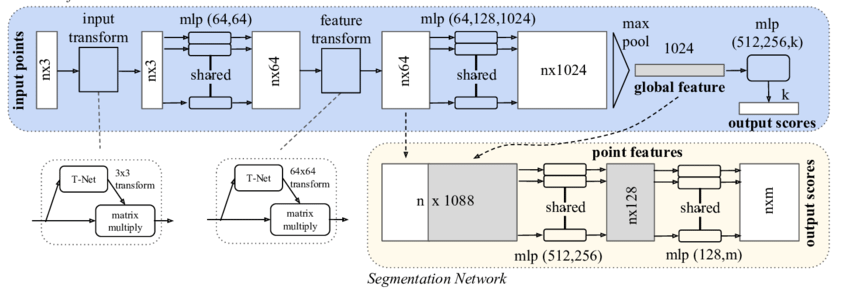
\includegraphics[width=\linewidth]{pointnet_architecture.png}
    \caption{PointNet Architecture for Classification and Segmentation \cite{qi2017pointnet}.
    \textit{mlp} indicates multi-layer perceptron; numbers in brackets are the layer sizes.}
    \label{fig:pointnet-architecture}
\end{figure}

Feature and input transformations are significant to the architecture, and is additionally described under permutation and transformation invariance. 

\subsection{Permutation Invariance}
Point clouds are unstructured, numerical sets and invariant to permutations ie., for $N$ points, there are $N!$ valid permutations (section \ref{sec:concepts-pointset}). Symmetric functions are therefore used to make PointNet invariant to input permutations \cite{qi2017pointnet}. Specifically, max pooling is used when \texttt{n} input points are mapped to higher dimensional space and then used directly for classification \cite{qi2017pointnet}. This can be seen in Figure \ref{fig:pointnet-symmetric}

\begin{figure} [ht!]
    \centering
    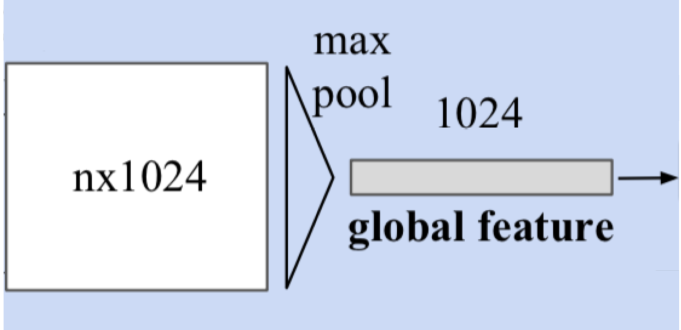
\includegraphics[width=0.5\linewidth, height=3cm,keepaspectratio]{symmetric_function.png}
    \caption{Symmetric Function with Max Pool Applied to Global Features \cite{qi2017pointnet}}
    \label{fig:pointnet-symmetric}
\end{figure}

\subsection{Transformation Invariance}
Point clouds must be invariant to certain geometric transformations (section \ref{sec:concepts-pointset}). If point clouds undergo transformation, then it is necessary that the classification labelling must be invariant as well. To ensure that this is the case, input and feature transformation sub-networks are used to provide normalisation to objects. \textit{T-Net} - a regression network is tasked with predicting a $n{\times}n$ transformation matrix.  

\begin{figure}[ht]   
\centering
\subfloat[Input Transformation]{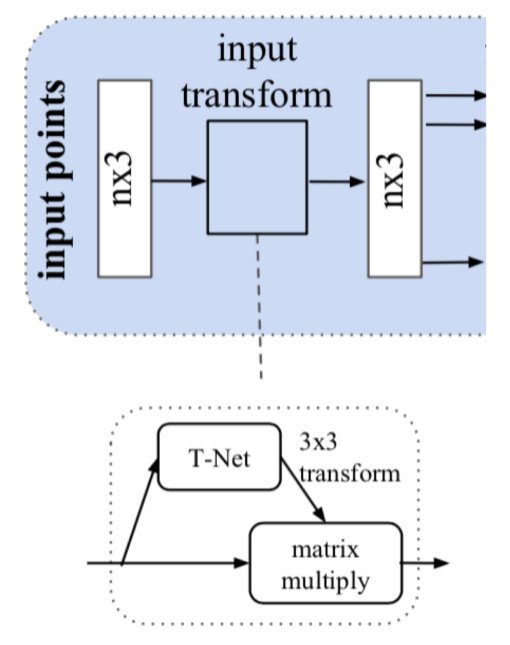
\includegraphics[width=0.4\textwidth, height=5.1cm,keepaspectratio]{input_transform.png}\label{fig:input_transform}}
\subfloat[Feature Transformation]{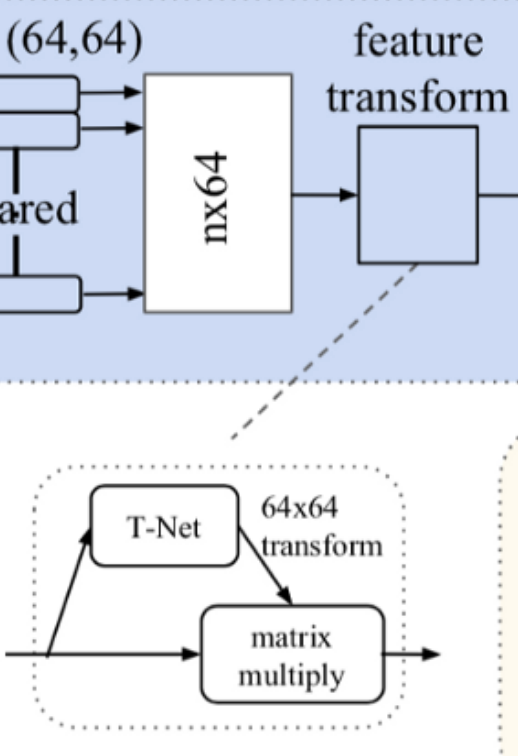
\includegraphics[width=0.4\textwidth,
height=5cm,keepaspectratio]{feature_transform.png}\label{fig:feature_transform}}
\caption[]{Input and Feature Transforms within PointNet}
\label{fig:input_feature_transform}
\end{figure}

For input transformations, \textit{n} input points are represented as a vector and  mapped to the embedding spaces. Geometric transformation then becomes easy to apply and involves matrix multiplying each point with a transformation matrix. Here, the T-Net predicts a $3{\times}3$ transformation matrix, which is then matrix multiplied with the $n{\times}3$ input (Figure \ref{fig:input_feature_transform}).

For feature transformation of the 64-dimensional embedding space, the corresponding T-Net predicts a $64{\times}64$ transformation matrix (Figure \ref{fig:input_feature_transform}). The increased number of trainable parameters leads to the potential for overfitting and instability during training, so a regularisation term is added to the loss function to constrain the feature matrix to be close to the orthogonal matrix:

\begin{equation}
    \mathcal{L}_{reg} = || I - AA^{T} ||^{2}_{F}
\end{equation}

where \textit{A} is the matrix predicted by the T-Net. 

So, PointNet is capable of learning from unordered, raw point clouds as long as the properties of point sets are maintained. This is relevant to the thesis and validated when preparing training data. Additional transformation functions within the network further ensure that the data respects invariance to permutations and transformations. These concepts are used by this thesis in the upcoming pipeline to ensure absolute accordance with rules governing point sets. 


\chapter{Data Generation and Exploration}
\label{sec:exploration}
\ifpdf
    \graphicspath{{4_data_exploration/figures/PNG/}{4_data_exploration/figures/PDF/}{4_data_exploration/figures/}}
\else
    \graphicspath{{4_data_exploration/figures/EPS/}{4_data_exploration/figures/}}
\fi


Nikhef provided simulated data from three sources that were used to generate the complete KM3NeT dataset - the \textit{K40 noise generator}, \textit{HDF5 hits and events} tables and a \textit{positions} file. This chapter describes the steps taken to combine noise and events data to produce the complete dataset. The chapter then discusses the quality and properties of the complete dataset by means of visual data exploration. 

\section{Noise Generation}
Noise for the dataset was generated using the \textit{k40gen} \footnote{https://gitlab.nikhef.nl/roelaaij/k40gen} package. \textit{k40gen} is a standalone background noise generator developed by Nikhef to generate a random array simulating Potassium-40 decay underwater. An instance of the generator was created with two random seeds - \texttt{21341} and \texttt{1245}. \texttt{7000}, \texttt{700}, \texttt{70}, and \texttt{0} were specified as the rates at which single, double, triple, and quadruple hits were to be generated respectively. Noise hits were generated from \texttt{0} nanoseconds (ns) till \texttt{100000000} ns. The ORCA (Oscillation Research with Cosmics in the Abyss) counting scheme was also provided as a numbering scheme for the photomultiplier (PMT) IDs within the Digital Optical Modules (DOMs). The DAS-5 cluster \footnote{https://www.cs.vu.nl/das5/} was used to install and generate the background noise array, totalling 5GB. The returned array contained information regarding \texttt{time}, \texttt{DOM ID}, \texttt{PMT ID} and \texttt{time-over-threshold} for noise hits.

Additionally, the positions file (\texttt{positions.detx}) contained all the spatial positions corresponding to the noise hits from the \textit{k40gen} array and had to be merged. Spatial positions from \texttt{positions.detx} were identified and mapped to the corresponding noise hits using the following formula:

\begin{equation}
    noise[pos\_idx] = 31 \times (noise[dom\_id] - 1) + noise[pmt\_id])
\end{equation}

Finally, a class label of \texttt{0} was also added for all hits to indicate noise for future classification. 


\section{Event Hits Generation}
Neutrino events data was stored in a HDF5 (Hierarchical Data Format version 5) file \footnote{https://www.hdfgroup.org/solutions/hdf5/} consisting of an event hits table (\texttt{mc\_hits}) and a corresponding event information table (\texttt{mc\_info}). \texttt{mc\_hits} included information pertaining to the DOMs (\texttt{dom\_id}), PMTs (\texttt{pmt\_id}),  positions (\texttt{pos\_x, pos\_y, pos\_z}) and directions (\texttt{dir\_x, dir\_y, dir\_z}) of event hits. It also contained time over threshold (\texttt{tot}) values and the time the hits were registered (\texttt{time}). A class label of \texttt{1} was added to this data to indicate an event hit. Only the \texttt{mc\_hits} table was used for the classification project undertaken in this thesis. 


\section{Data Combination}
Before the background noise and event hits data could be combined, a few preliminary cleanup and validation measures were taken. First, it was noticed that the PMT IDs for event hits were from \texttt{0} till \texttt{6417}. This indicated that it followed a global numbering scheme, while PMT IDs for noise hits had been generated using the ORCA numbering scheme. To enforce uniformity, PMT IDs for event hits were set from \texttt{1} till \texttt{31}: 

\begin{equation}
    pmt\ id = pmt\ id - 31 \times (dom\ id - 1)
\end{equation}

Next, \texttt{time} for some noise hits were negative, so these data points were deemed invalid and deleted from the dataset. As both events and noise data were simulated, it was important to ensure that the \texttt{time} values associated with event hits were not biased. To check for such a bias, the mean time of occurrence for all event hits was calculated and plotted for any evidence of hits clusters. Based on the evenly distributed scatter of points in Figure \ref{fig:bias_verification}, it was concluded that there were no biases in the data. Noise and event hits were merged to form the complete KM3NeT dataset after negative time was deleted, PMT IDs were adjusted and data validity was confirmed.

\begin{figure}[ht!]
    \centering
    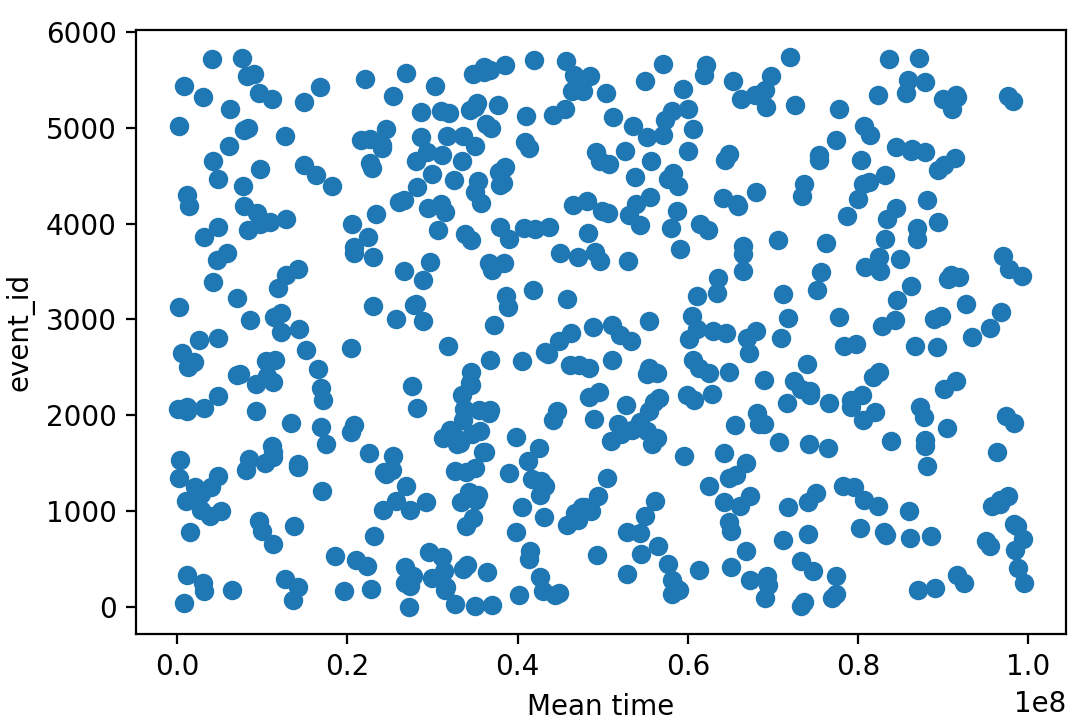
\includegraphics[width=0.7\textwidth, height=7cm]{bias_verification.png}
    \caption{Scatter Plot of Mean Time for All Event Hits}
    \label{fig:bias_verification}
\end{figure}



\section{Key Attributes}
The KM3NeT detector records and sends data in chunks (timeslices) for processing at the offshore facility \cite{km3net_2017}. The thesis's main aim was to train a network that would classify timeslices into those that contained only noise and those that contained event hits amidst noise. Therefore, the dataset was sequentially binned into groups of 15000 ns and assigned a number for identification. For example, timeslice \texttt{0} contained all hits that occurred between 0 ns and 15000 ns. 15000 ns was used for binning as neutrino events typically occur between 100 ns and 15000 ns \cite{km3net_2017}. Selecting a value on the higher end of the range allowed for fewer groups to be created and by extension, faster processing. The binning resulted in a total of 6759 groups. The complete dataset was found to be 4GB in size, with 45,820,220 rows and 12 attributes, summarised in Table \ref{tab:attributes}.

\begin{table} [ht!]
    \begin{tabular}{l l}
    \hline
        \textbf{Attribute} & \textbf{Description} \\
    \hline
       \texttt{dom\_id} & [Unique ID for sensor module.] \\
       \texttt{pmt\_id} & [Unique ID for photomultiplier (PMT) tubes within DOMs.] \\
       \texttt{pos\_x, pos\_y, pos\_z}  & [Spatial coordinates (in meters) of hit within the detector.] \\
       \texttt{dir\_x, dir\_y, dir\_z} & [Direction of PMT tubes within DOMs to look for \\
                                       & Cherenkov Light.] \\
       \texttt{tot}   & [Time-over-threshold (ToT) indicates the amount of light \\
                      & transformed to charge which is interpreted as the length \\
                      & of the square wave pulse over a given threshold \cite{karas_2019}.] \\
       \texttt{time}  & [Time at which the hit was recorded.]\\
       \texttt{label} & [0 or 1 class label indicating whether hit is from noise or \\
                      & event respectively.]\\
       \texttt{group} & [Timeslice numbers starting from 0 for the purpose \\
                      & of identification.] \\
    \hline
    \end{tabular}
    \caption{KM3NeT Data Attributes and Description}
    \label{tab:attributes}
\end{table}


Domain knowledge from Nikhef indicated \texttt{dom\_id, pmt\_id} and direction of PMT tubes (\texttt{dir\_x, dir\_y, dir\_z}) to be metadata that could be ignored. Additionally, work by Karas (2019) identified time-over-threshold (\texttt{tot}) to be insignificant to the classification problem \cite{karas_2019}. The remaining attributes - spatial coordinates (\texttt{pos\_x, pos\_y, pos\_z}), \texttt{time}, \texttt{label} and timeslices (\texttt{group}) were identified as key variables for the remainder of the classification project. 


\section{Visual Analysis}

\begin{figure}[ht!]
    \centering
    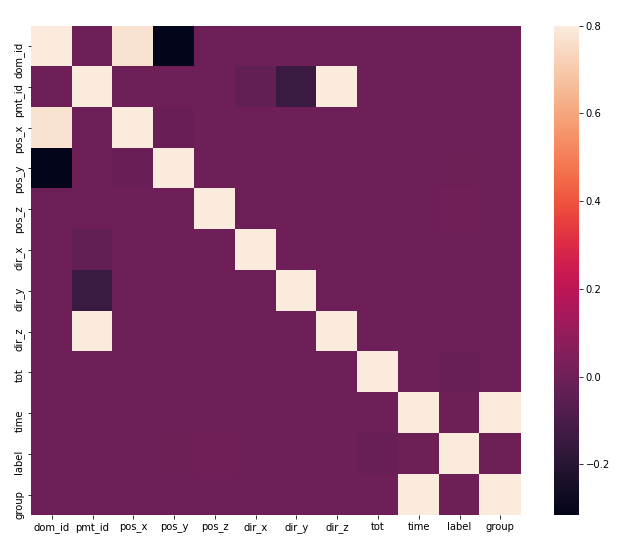
\includegraphics[width=0.7\linewidth, height=7cm]{correlations.png}
    \caption{Correlation Heatmap Between Variables}
    \label{fig:corr}
\end{figure}

Python libraries were used to explore the quality of the dataset and gain further insight on the key variables and the relationships that may exist between them. The dataset was found to have no missing values or outliers. All hits occurred between \texttt{0} ns till \texttt{101591357} ns. The dataset showed severe imbalance between event hits and noise as, for every 1 event hit, there were 93 noise hits. Finally, the correlation heatmap in Figure \ref{fig:corr} indicated that the key variables had no relevant relationship with each other. Significant variables were further examined to identify existence of useful properties.


\subsubsection*{Timeslices (\texttt{group}):} 
Timeslice \texttt{0} was found to have the highest number of hits (12,454), all of which were noise. Timeslice \texttt{615} contained the highest number of event hits (around 8500) with the lowest noise-to-event hits ratio of 4:1. Figure \ref{fig:points_per_group} shows the distribution of number of points per timeslice. Timeslice \texttt{0} had the highest occurrence of hits while some timeslices contained very few hits. These timeslices were edge cases and were ignored for the rest of the project. However, majority of the other timeslices contained between 6000 to 8000 hits, providing a more or less consistent sample for the training.

\begin{figure}[ht!]
    \centering
    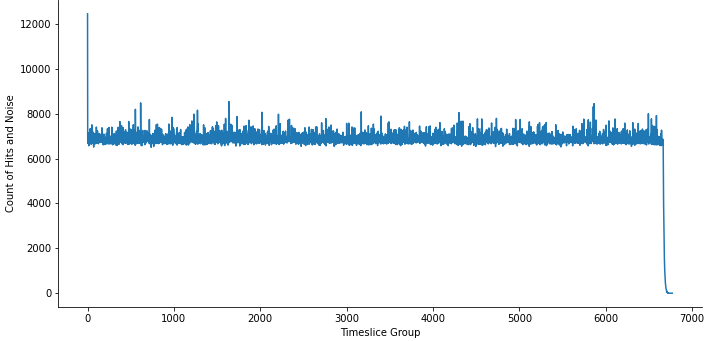
\includegraphics[width=0.7\linewidth, height=5cm,keepaspectratio]{points_per_group.png}
    \caption{Count of Total Points per Timeslice}
    \label{fig:points_per_group}
\end{figure}

In accordance with the classification task, timeslices were separated into those that contained only noise and those that contained both event hits and noise. First, class imbalance between event hits and noise within timeslices were visually examined. Figure \ref{fig:hits_by_group} shows that most timeslices with both events and noise had between 0 to 250 event hits. On the other hand, Figure \ref{fig:noise_by_group} shows noise timeslices had around 7000 points on average. The outliers in this Figure (\ref{fig:noise_by_group}) demonstrate a timeslice that had a significantly large number of noise hits and timeslices towards the end that had comparatively fewer noise hits. These anomalies could be attributed to the nature of the \textit{k40gen} random noise generator. Figure \ref{fig:kde_hits_by_group} and Figure \ref{fig:kde_noise_by_group} use kernel density estimation (KDE) to produce a continuous density estimate using a Gaussian Kernel and provides an alternate visualisation of the severe class imbalance by highlighting the densest regions \cite{waskom2020seaborn}.


\begin{figure}[ht!]   
\centering
\subfloat[Count of Event Hits For Timeslices with Both Noise and Events]{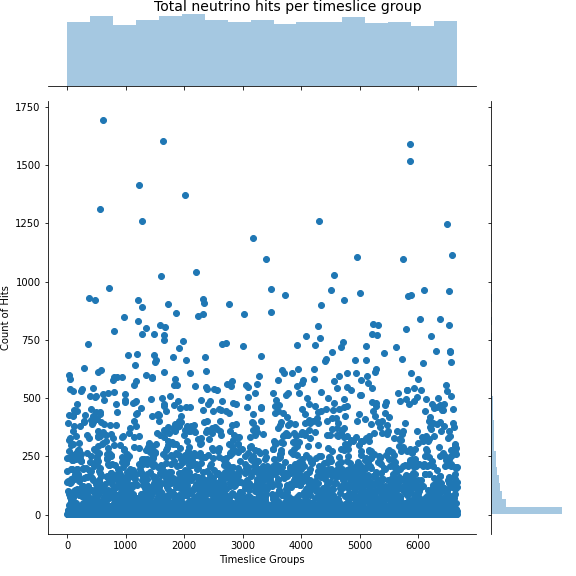
\includegraphics[trim={0 0 0 0.51cm}, clip, width=0.5\textwidth, keepaspectratio]{hits_by_group.png}\label{fig:hits_by_group}}
\subfloat[Count of Noise Hits For Timeslices with Only Noise]{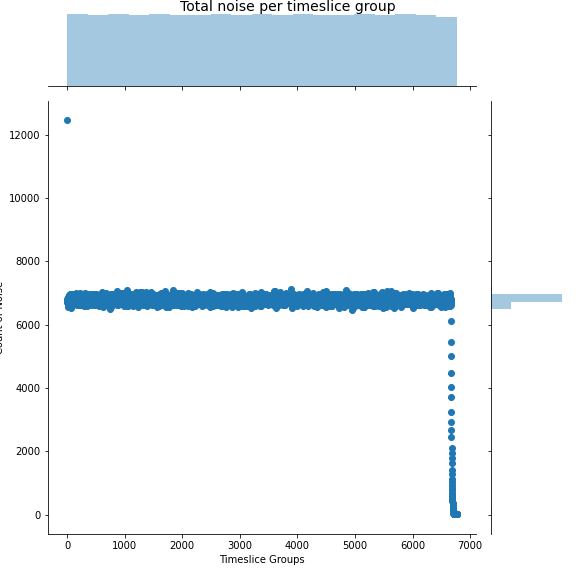
\includegraphics[width=0.5\textwidth,
height=7.4cm,keepaspectratio]{noise_by_group.png}\label{fig:noise_by_group}}

\subfloat[Kernel Density Estimation for Only Event Hits]{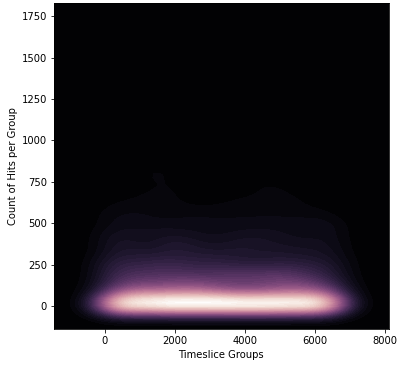
\includegraphics[trim={0 0 0 0.51cm}, clip, width=0.5\textwidth, keepaspectratio]{kde_hits_per_group}\label{fig:kde_hits_by_group}}
\subfloat[Kernel Density Estimation for Only Noise Hits]{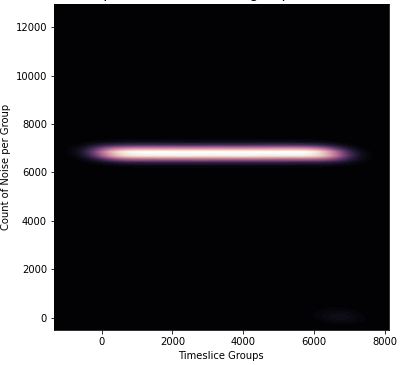
\includegraphics[width=0.5\textwidth,
height=7.4cm,keepaspectratio]{kde_noise_per_group}\label{fig:kde_noise_by_group}}
\caption{Comparing Count of Hits and Noise Between Timeslices}
\label{fig:kde_comparing_groups}
\end{figure}

\subsubsection*{3D Spatial Coordinates (\texttt{pos\_x, pos\_y, pos\_z}):} 
Figure \ref{fig:615_points} uses a "swarm" technique to show distribution of noise and event hits across time for timeslice \texttt{615}, the group with the highest incidence of event hits. The points are non-overlapping and adjusted to better show distribution \cite{waskom2020seaborn}. Orange points indicate that event hits occur in groups coinciding with neutrino events amidst the noise. 

\begin{figure}[ht!]
    \centering
    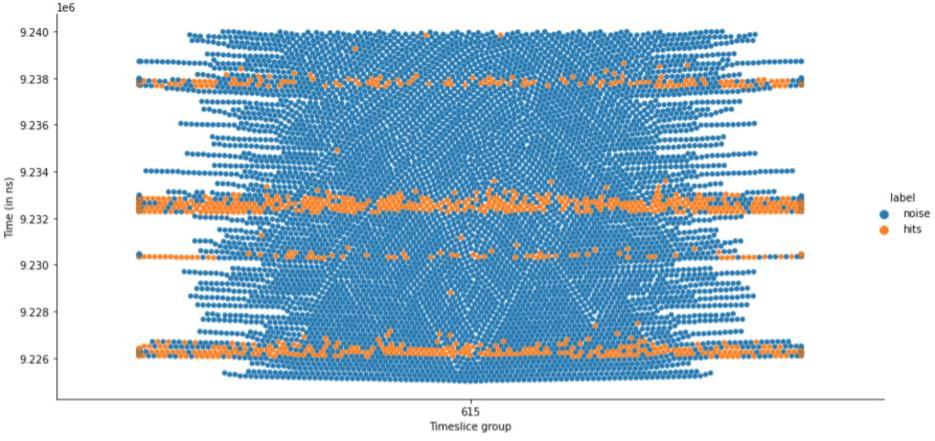
\includegraphics[width=0.7\linewidth,keepaspectratio]{615_point_distribution.jpg}
    \caption{Distribution of Noise and Event Hits in Timeslice 615}
    \label{fig:615_points}
\end{figure}

Bi-variate plots in Figure \ref{fig:x_y_z} show the relationship between the \texttt{x, y, z} points for timeslice \texttt{615}. These 3D coordinates don't give much information or patterns that may indicate presence of event hits, confirming the need for \texttt{time} as part of the dataset.

\begin{figure}[ht!]   
\centering
\subfloat[Scatter plot for \texttt{pos\_x} against \texttt{pos\_y}]{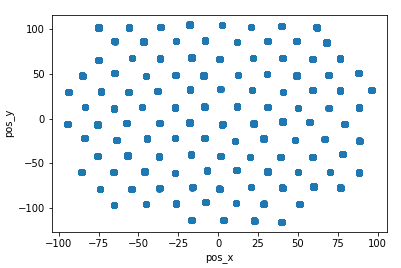
\includegraphics[width=0.33\textwidth,height=5cm]{x_y.png}\label{fig:xy}}
\subfloat[Scatter plot for \texttt{pos\_x} against \texttt{pos\_z}]{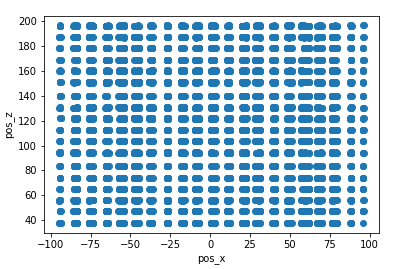
\includegraphics[width=0.33\textwidth,
height=5cm]{x_z.png}\label{fig:xz}}
\subfloat[\texttt{pos\_y} against \texttt{pos\_z}]{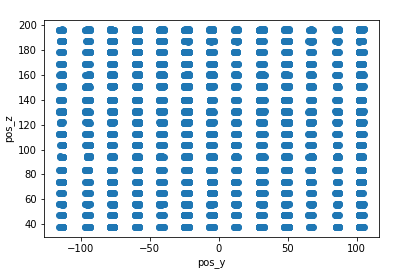
\includegraphics[width=0.33\textwidth,
height=5cm]{y_z.png}\label{fig:yz}}
\caption[]{Bi-variate Plots Showing Relationship Between 3D Coordinates}
\label{fig:x_y_z}
\end{figure}

Figure \ref{fig:fig:0_615} shows an enhanced 3D render of timeslice \texttt{615} generated using MeshLab \footnote{https://www.meshlab.net/}. The timeslice is first visualised as \texttt{x}, \texttt{y} and \texttt{time}, then \texttt{x, z} and  \texttt{time} and finally \texttt{y, z,} and \texttt{time}.  The three representations show no relevant differences between each other. However, visual enhancements via MeshLab allow for event clusters to stand out, as indicated by the bright clusters of points.

\begin{figure}[ht!]   
\centering
\subfloat[3D Plot of \texttt{x, y, time}]{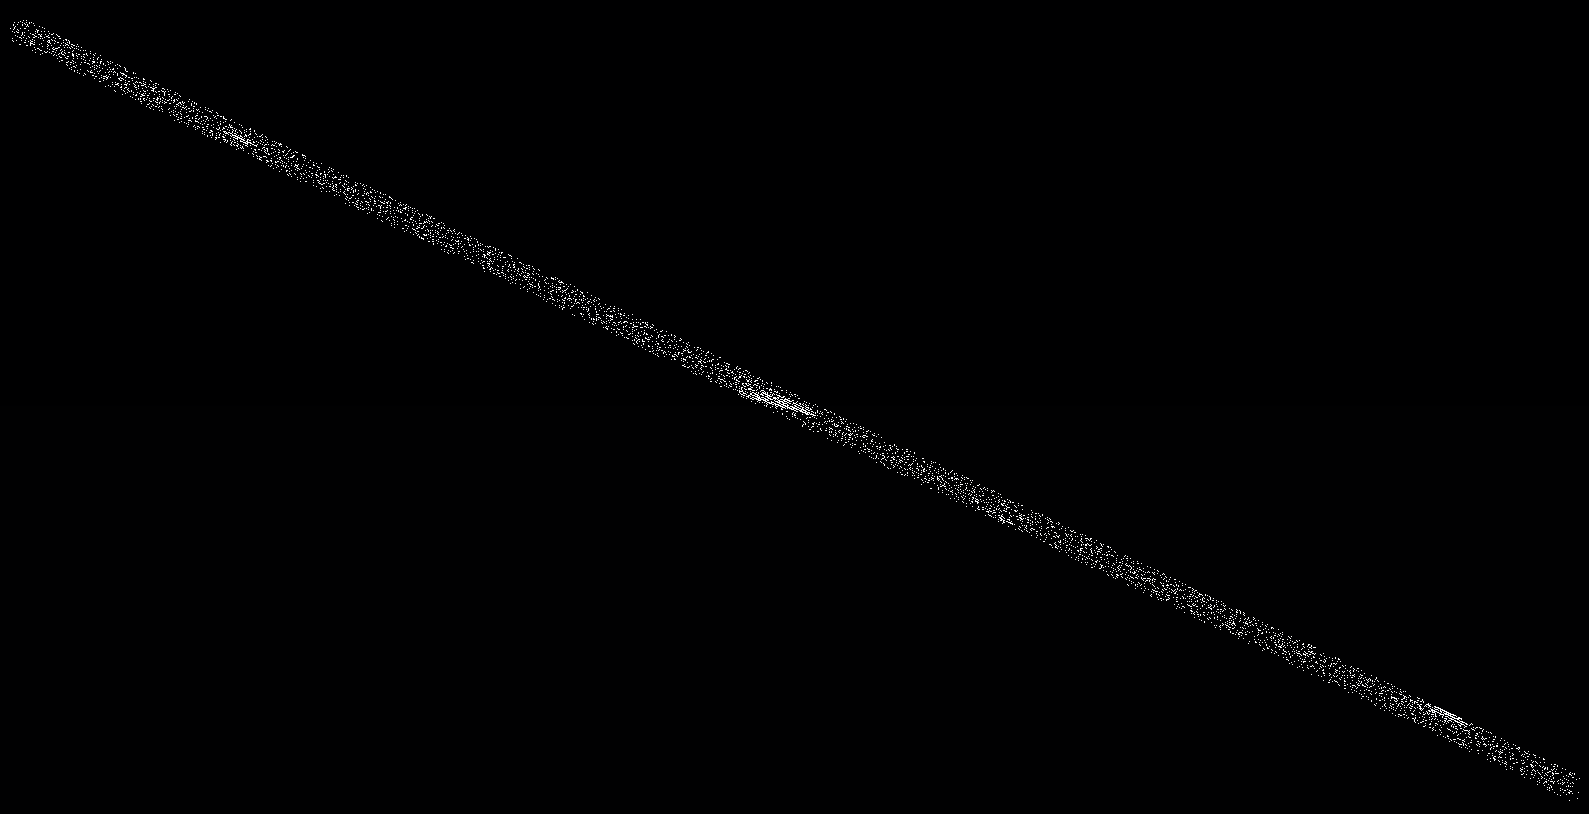
\includegraphics[width=0.32\textwidth,height=5cm]{xyt.png}\label{fig:xyt}}
\hspace{0.01cm}
\subfloat[3D Plot of \texttt{x, z, time}]{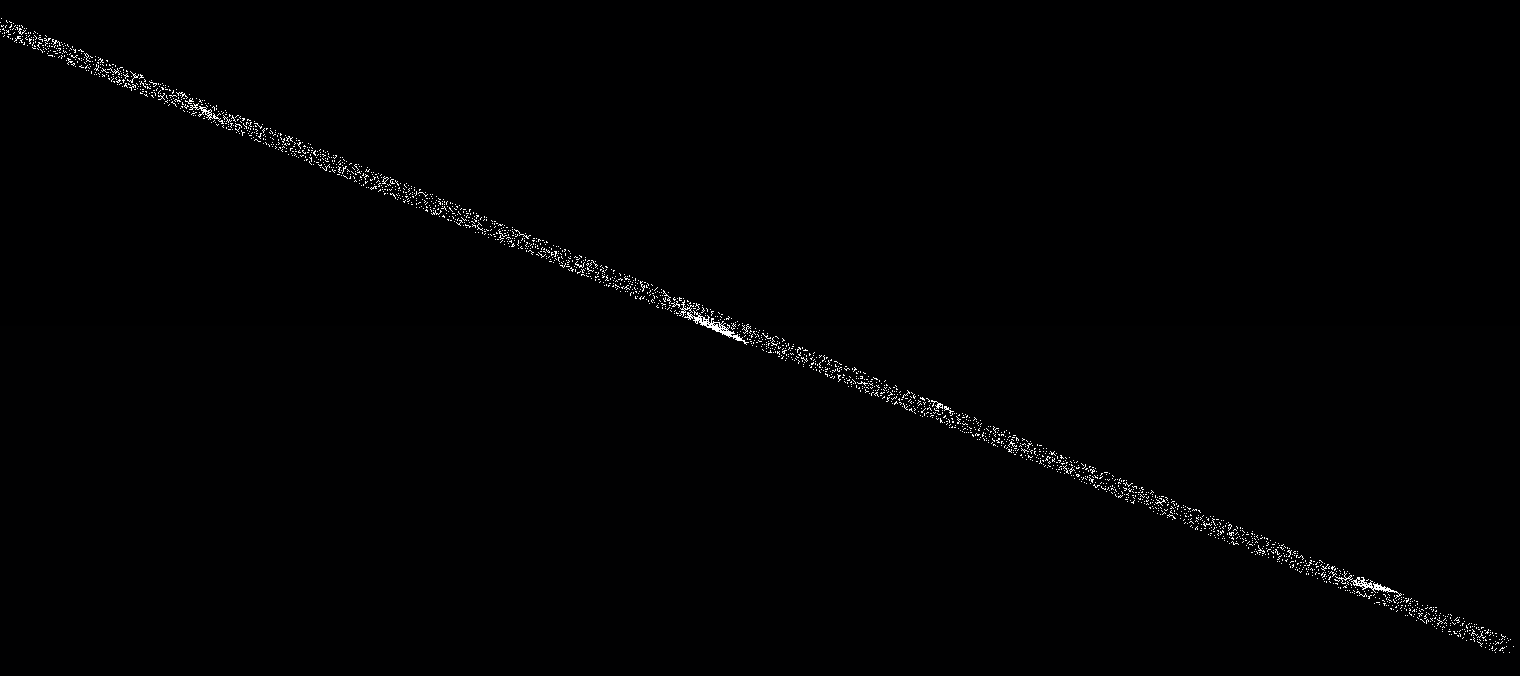
\includegraphics[width=0.32\textwidth,height=5cm]{xzt.png}\label{fig:xzt}}
\hspace{0.01cm}
\subfloat[3D Plot of \texttt{y, z, time}]{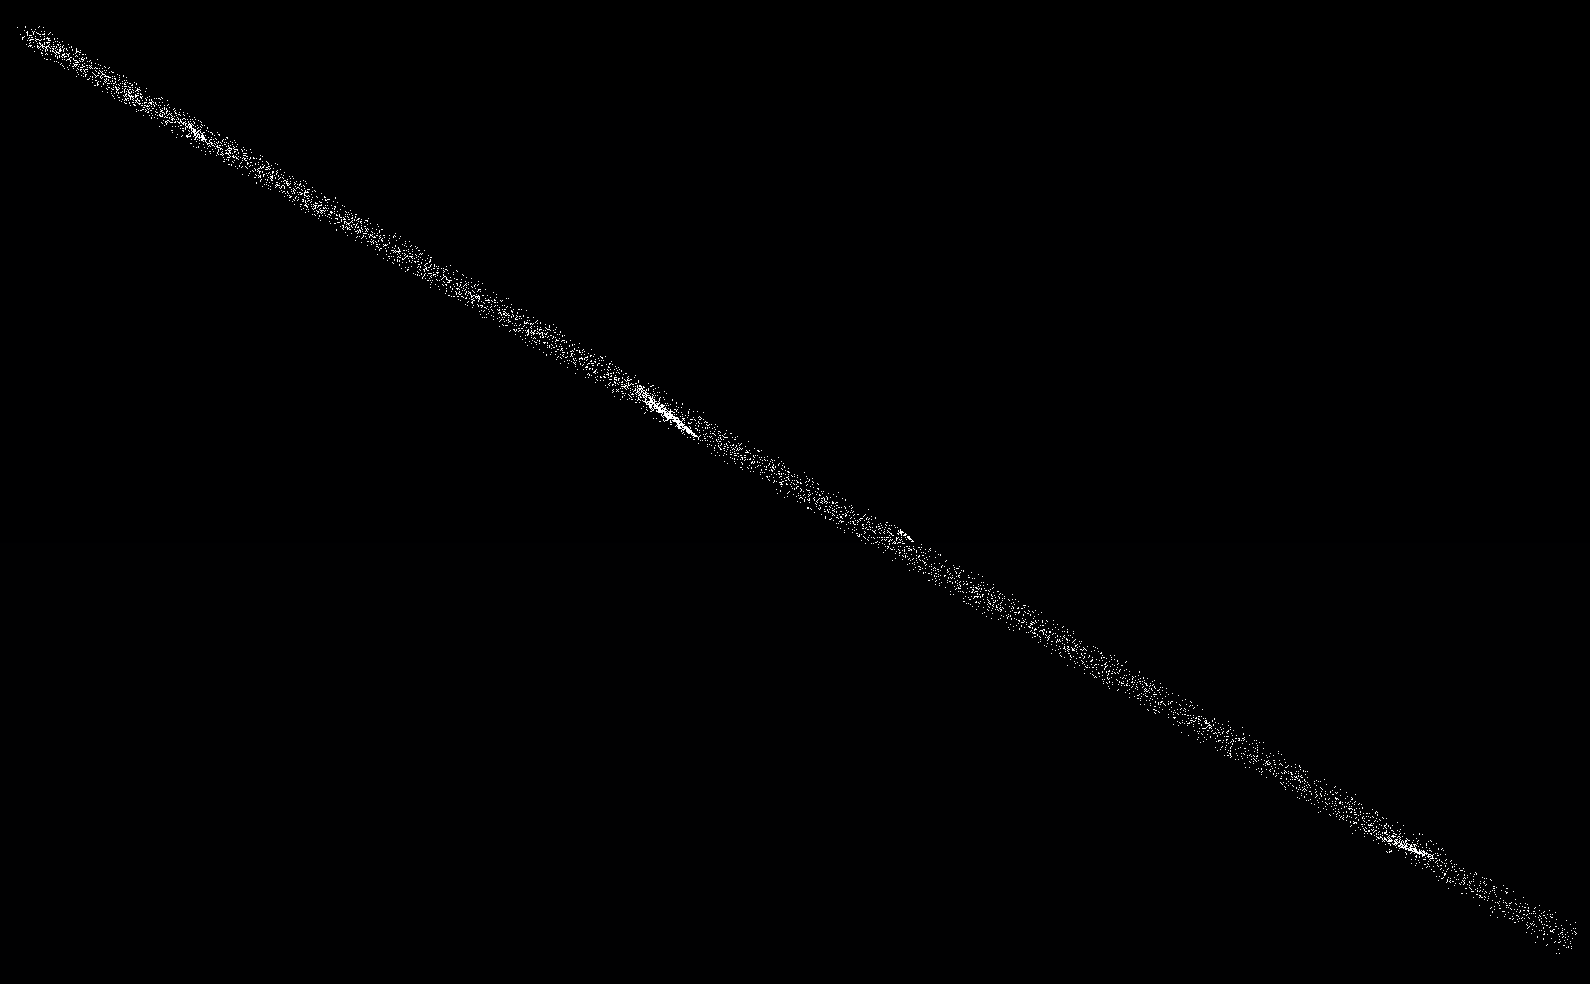
\includegraphics[width=0.32\textwidth,height=5cm]{yzt.png}\label{fig:yzt}}
\caption[]{3D Plots Showing Combinations of \texttt{x, y, z, time} for Timeslice 615}
\label{fig:fig:0_615}
\end{figure}

\subsection*{Time (\texttt{time})}
Time plays a significant role in the identification of neutrino hits amidst noise. A swarm plot of \texttt{time} against \texttt{label} was plotted for two events timeslices to note the relation between time and type of hit \cite{eklund2012beeswarm}. Figure \ref{fig:time} shows an even distribution of noise hits across time, while event hits again form localised clusters.

\begin{figure}[ht!]   
\centering
\subfloat[\texttt{time} and \texttt{label} for Timeslice 615]{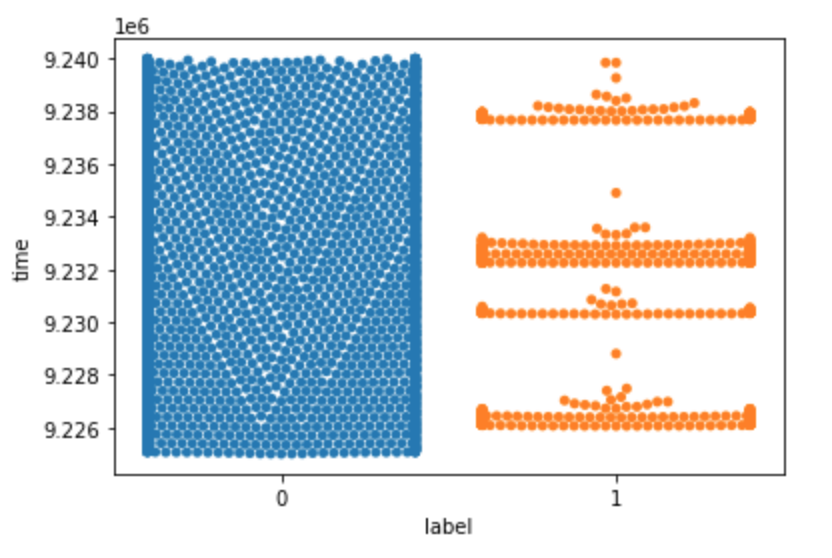
\includegraphics[width=0.5\textwidth,height=10cm, keepaspectratio]{label_time_615.png}}
\subfloat[\texttt{time} and \texttt{label} for Timeslice \texttt{1637}]{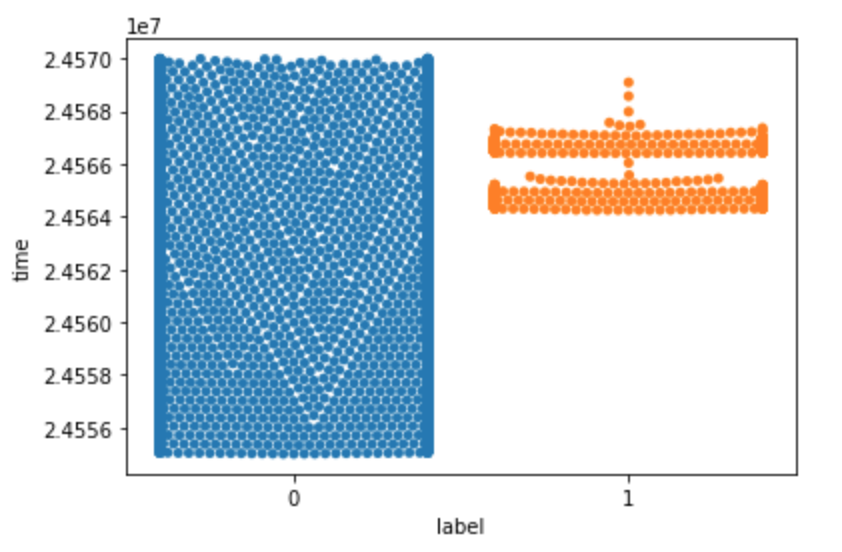
\includegraphics[width=0.5\textwidth,height=10cm, keepaspectratio]{time_label_1637.png}}
\caption[]{Swarm Plots Showing Relationship Between Time and Hit Labels}
\label{fig:time}
\end{figure}

Based on the combined results from plots of spatial positions, \texttt{time} and \texttt{label}, it was evident that a combination of these attributes would be required to obtain sufficient information on event hits. Further, the dataset had unrelated variables, lacked significant patterns, and had a high density of points. It would be very likely that the network would not be able to learn anything significant. Therefore, feature engineering may be required to add new information to the dataset before training could occur. 

\let\cleardoublepage\clearpage


\chapter{The Pipeline}
\label{sec:pipeline}

\ifpdf
    \graphicspath{{5_pipeline/figures/PNG/}{5_pipeline/figures/PDF/}{5_pipeline/figures/}}
\else
    \graphicspath{{5_pipeline/figures/EPS/}{5_pipeline/figures/}}
\fi

The design goal of the pipeline is to accept timeslices as input and output a \texttt{0} or \texttt{1} indicating whether they need to be discarded or saved respectively. Two classes were identified: \texttt{class\_0} comprised timeslices with just noise and \texttt{class\_1} included timeslices with event and noise hits. Henceforth, the thesis refers to \texttt{class\_1} timeslices as event timeslices, but they contain both noise and event hits.

Stakeholder knowledge and data exploration (Chapter \ref{sec:exploration}) identified 6 key variables - \texttt{pos\_x, pos\_y, pos\_z, time, group} (timeslice) and \texttt{label}. Since neutrinos are identified by both spatial and time differences between each other, an ideal dataset would contain all four variables \cite{km3net_2017}. However, generating a 4D mesh with \texttt{time} was not feasible, as the process is complicated and relatively under-developed \cite{otomo2014direct}. Instead, \texttt{time} was combined with spatial coordinates to create three permutations of the dataset - (\texttt{x, y, time}), (\texttt{x, z, time}) and (\texttt{y, z, time}). The following chapter discusses each component of the pipeline in detail. All three datasets were processed and transformed in the same manner, so details described in the following pipeline are applicable to all three datasets.

\section{Generation of Point Clouds}
The first step in the pipeline was to build 3D point clouds for each timeslice and save them as \texttt{.xyz} files. In order to do so, a few preliminary steps were undertaken. First, timeslices were divided into two classes whereby one contained only noise and the other contained both noise and event hits. Most timeslices with only noise had an average of 6500 hits per timeslice, but there were a few timeslices that had a single noise hit. Likewise, timeslices with event hits had an average of 6900 hits per timeslices, but some timeslices had only 3 event hits. Discussion with domain scientists indicated that such groups represented an unrealistic scenario. Therefore, they were excluded from the data as they would not be able to provide a quality training sample.

Figure \ref{fig:p0_countplot_ci} shows class imbalance before and after selection of the largest timeslices per class. It shows imbalance both across the noise and events class; and also within the events class. Sub-figure \ref{fig:p0_class_imbalance} shows that the noise timeslices had fewer noise hits compared to the noise hits in event timeslices. Moreover, within the event timeslices, there is significant disparity between the number of noise and event hits. Sub-figure \ref{fig:p0_class_imbalance} indicates that the class imbalance needed to be improved as it may affect training and bias the classifier towards the majority class. Further, the entire dataset was not required for training. So, in order to continue with a smaller, quality training data, the top 200 timeslices were taken for each class. For the events class, timeslices were sorted in a descending order based on the number of event hits they contained. The largest 200 of these timeslices were then selected. Similarly, the top 200 noise timeslices were also selected. 

\begin{figure}[ht!]   
\centering
\subfloat[Count of Noise and Event Hits from All Timeslices]{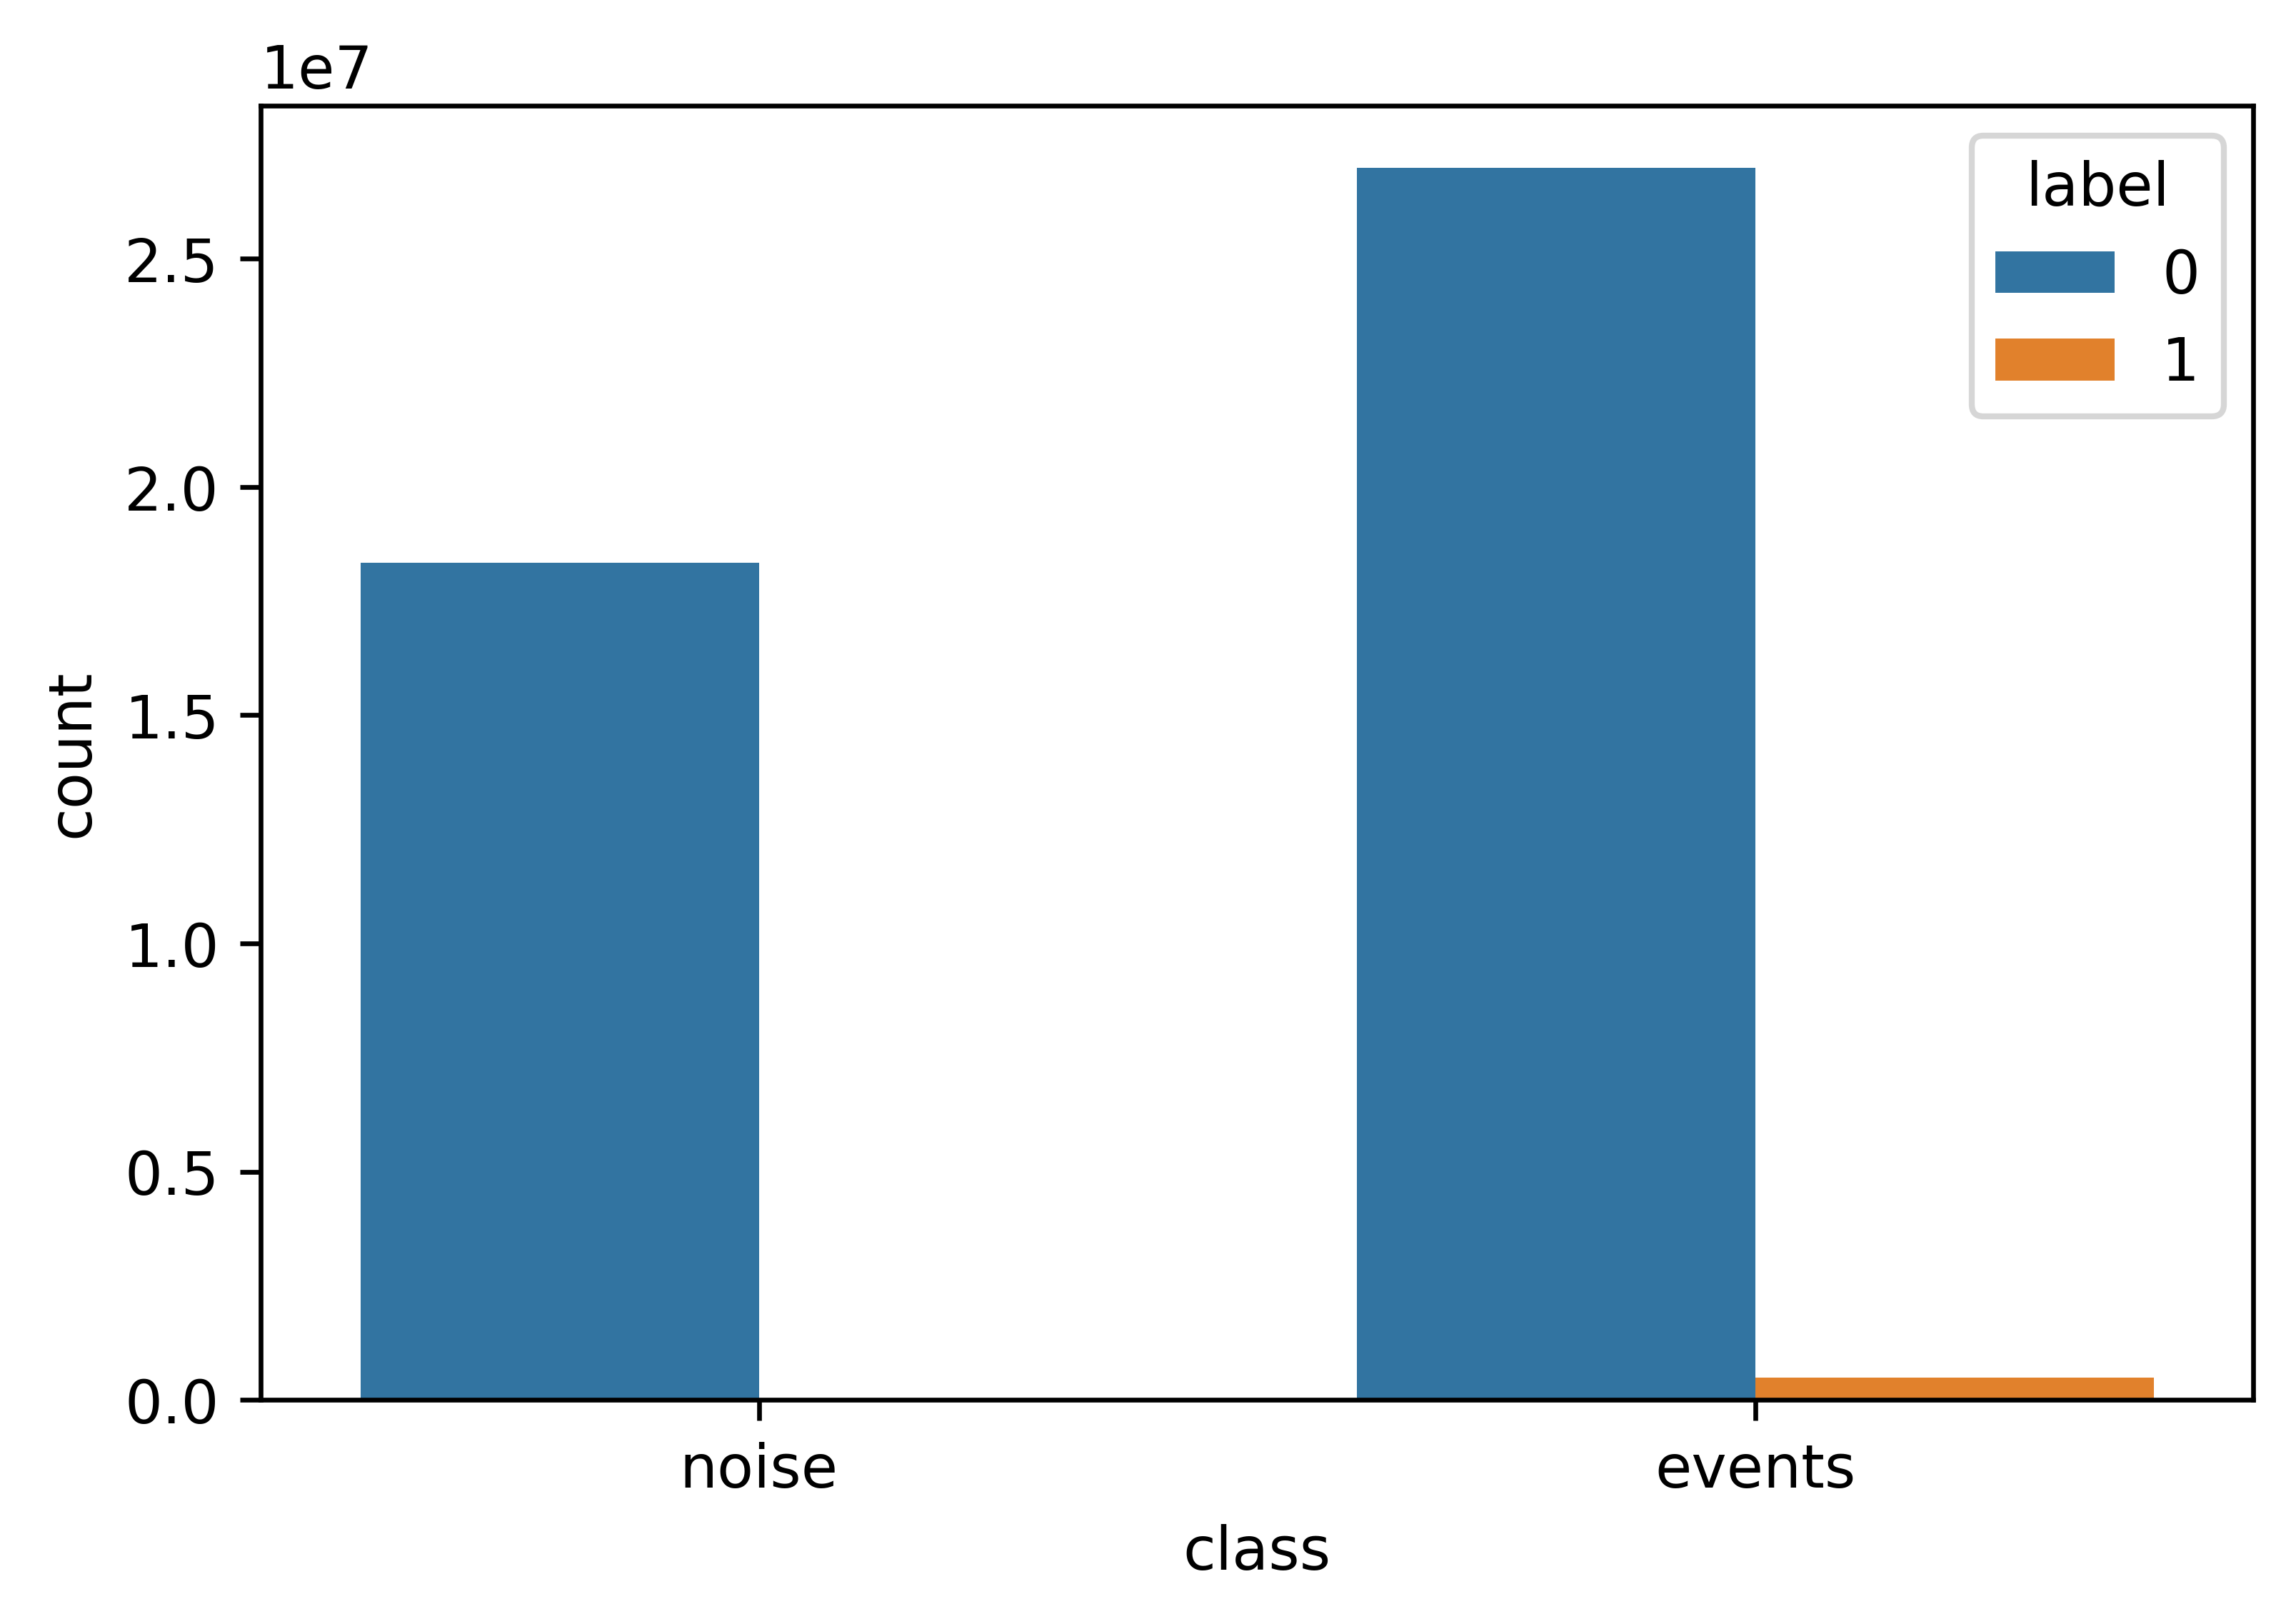
\includegraphics[width=0.48\textwidth, keepaspectratio]{class_imbalance}\label{fig:p0_class_imbalance}}
\subfloat[Count of Noise and Event Hits for 200 Noise and Event Timeslices]{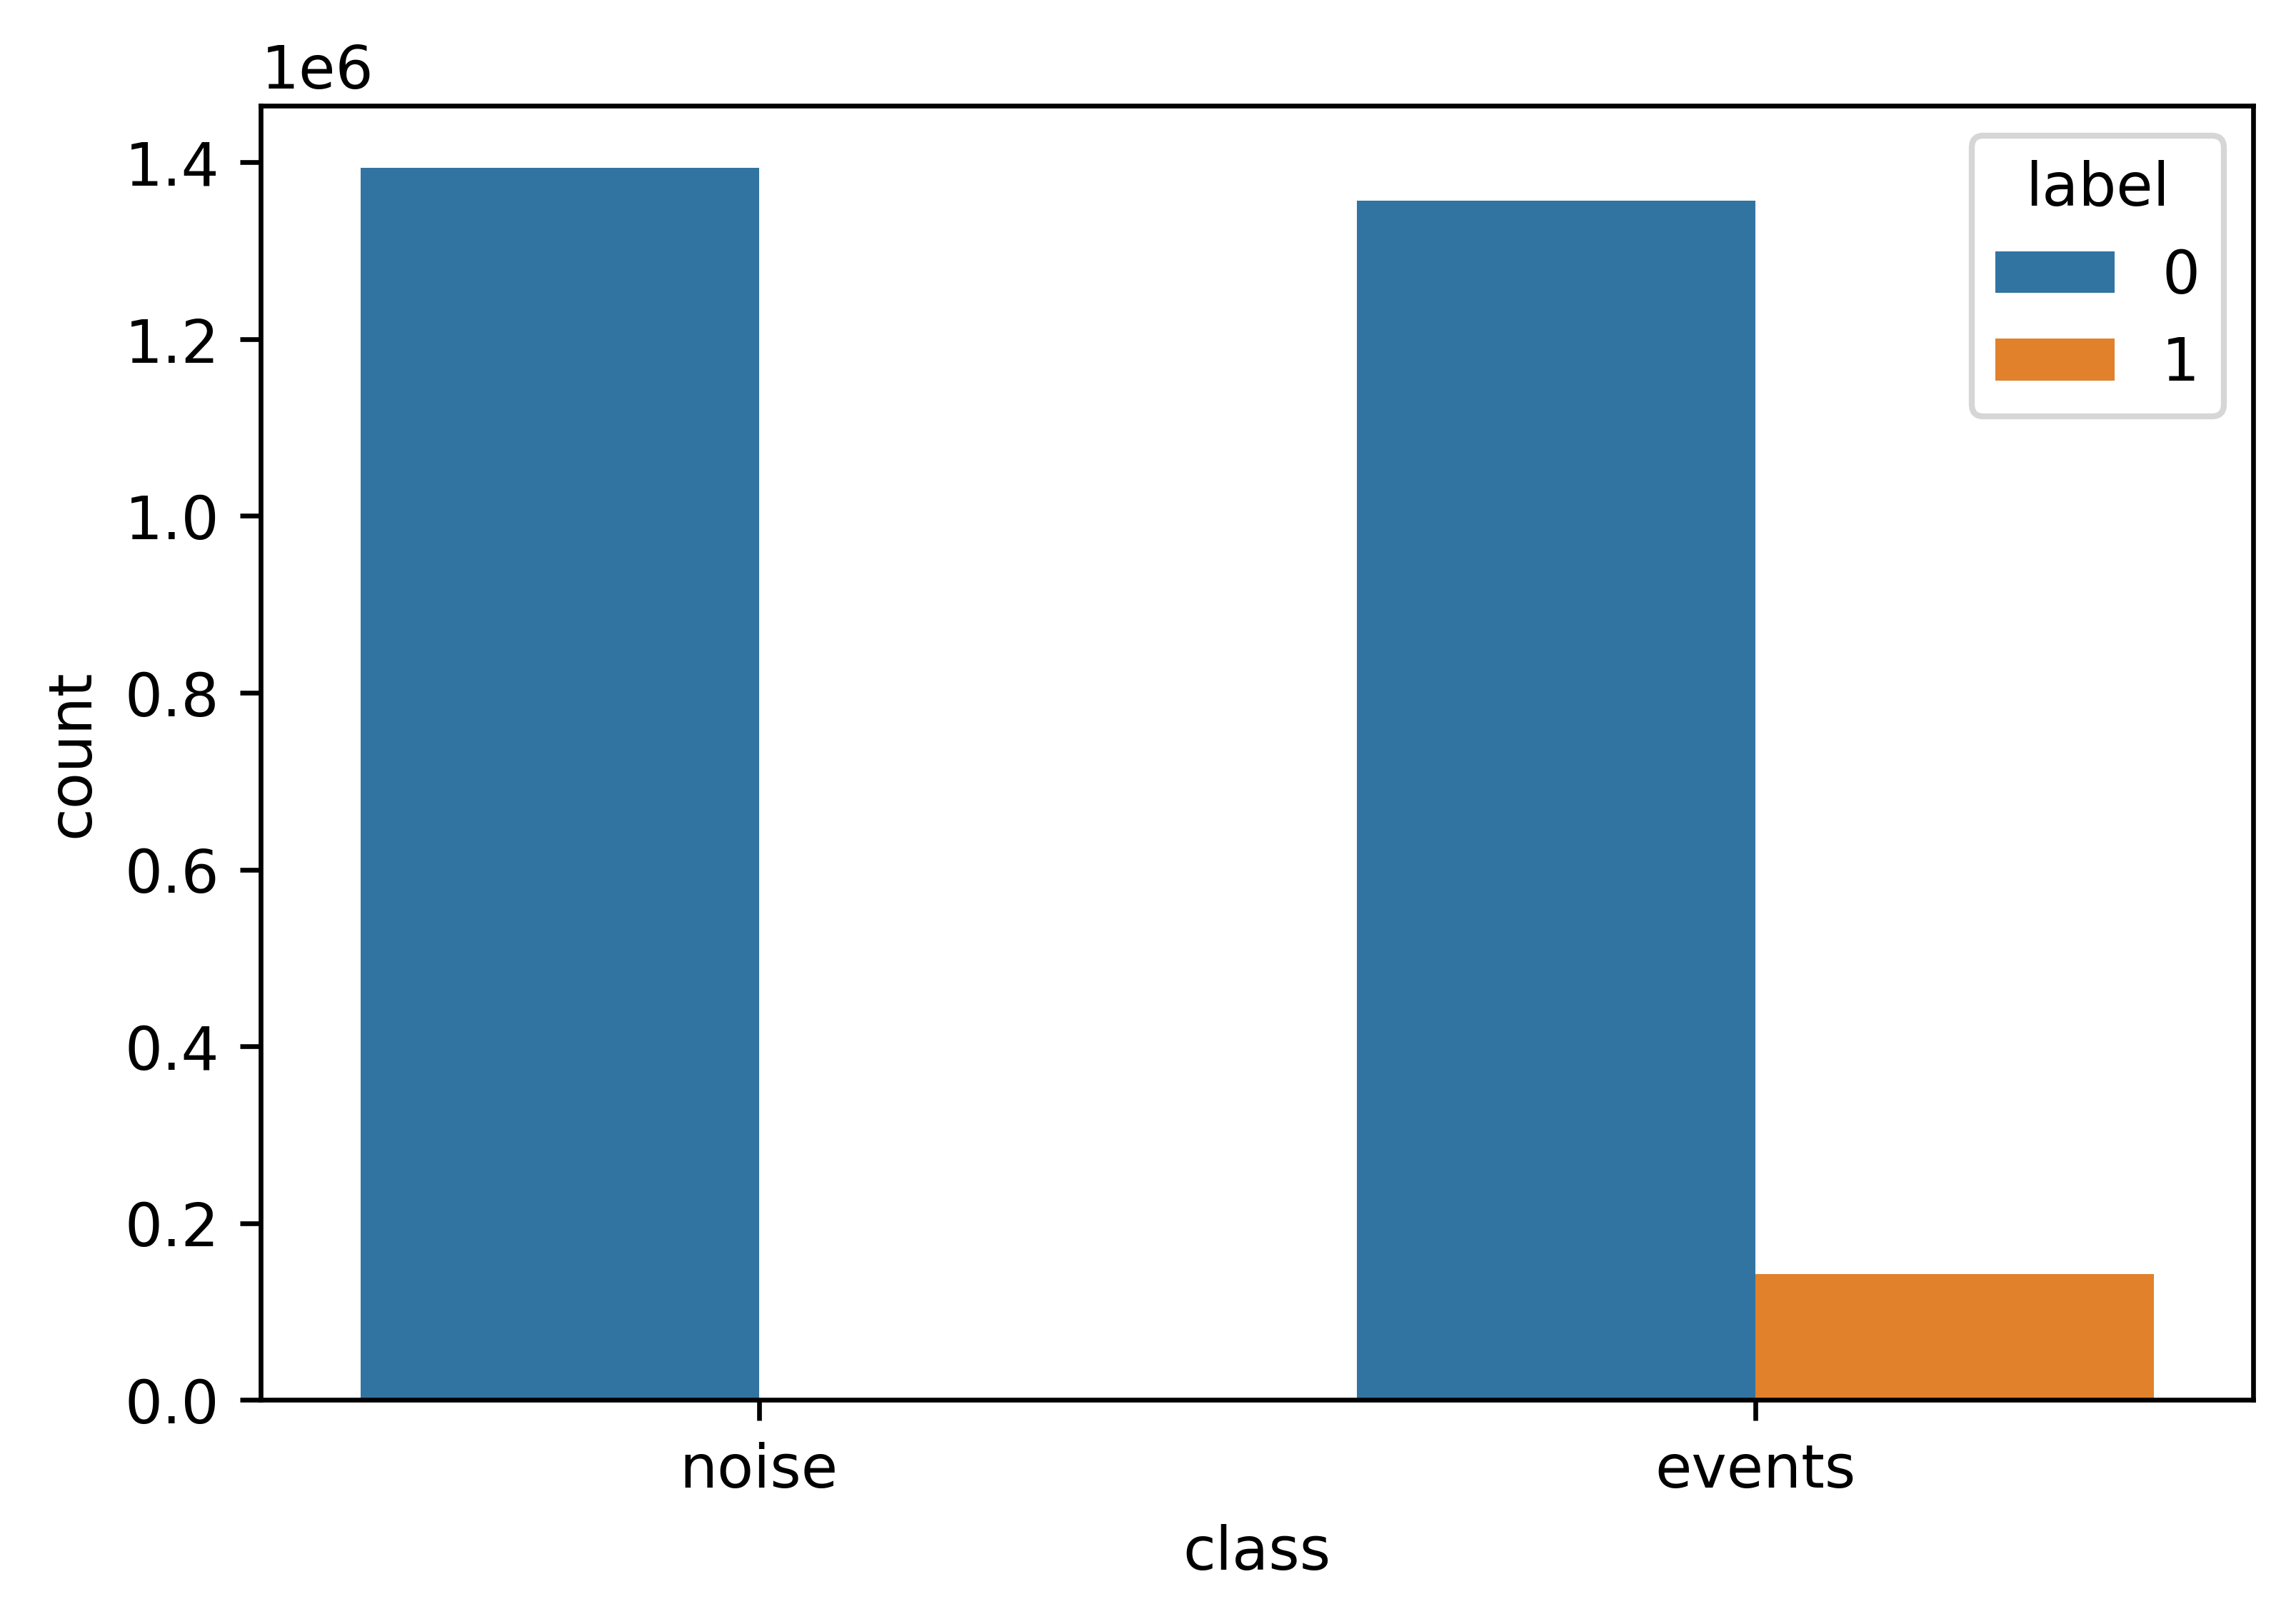
\includegraphics[width=0.48\textwidth, keepaspectratio]{class_imbalance_after_sampling}\label{fig:p0_200_class_imbalance}}
\caption[]{Class Imbalance Before and After Selection of Top 200 Timeslices Per Class}
\label{fig:p0_countplot_ci}
\end{figure}

Sub-figure \ref{fig:p0_200_class_imbalance} shows the class imbalance after selecting the top timeslices. The noise hits are now equal between the two classes. Further, there is some improvement between the event and noise hits within the events class. This indicated that taking the largest timeslices helped make the dataset more uniform and balanced for training.

Data for the 200 event timeslices were further observed. It was seen that there were a total of 27,485,996 hits, of which only 489,906 were event hits. Positive hits formed only 1.78\% of the data. The maximum number of hits a timeslice was 1692 and the smallest number of hits in a timeslice was 487. On average, timeslices had around 700 event hits. In contrast, these timeslices had 7000 noise hits on average. All timeslices were saved as point clouds under their respective classes - \texttt{class\_0} comprising of noise point clouds and \texttt{class\_1} comprising of event and noise point clouds.


\section{Feature Engineering}
Feature engineering is the process through which data can be transformed in a manner that either brings new information to light or provides more structure to the data, making learning easier for the network \cite{guyon2003introduction}. Feature engineering was included in the pipeline due to three main reasons.Visual data exploration (Section \ref{sec:exploration}) revealed unrelated variables with no significant patterns. Next, visual inspection of both point clouds and their corresponding 3D meshes showed lack of potential structure. Finally, preliminary results from training on data without feature engineering showed the need for additional information (Appendix \ref{appendix}).

\begin{figure}[ht!]
    \centering 
    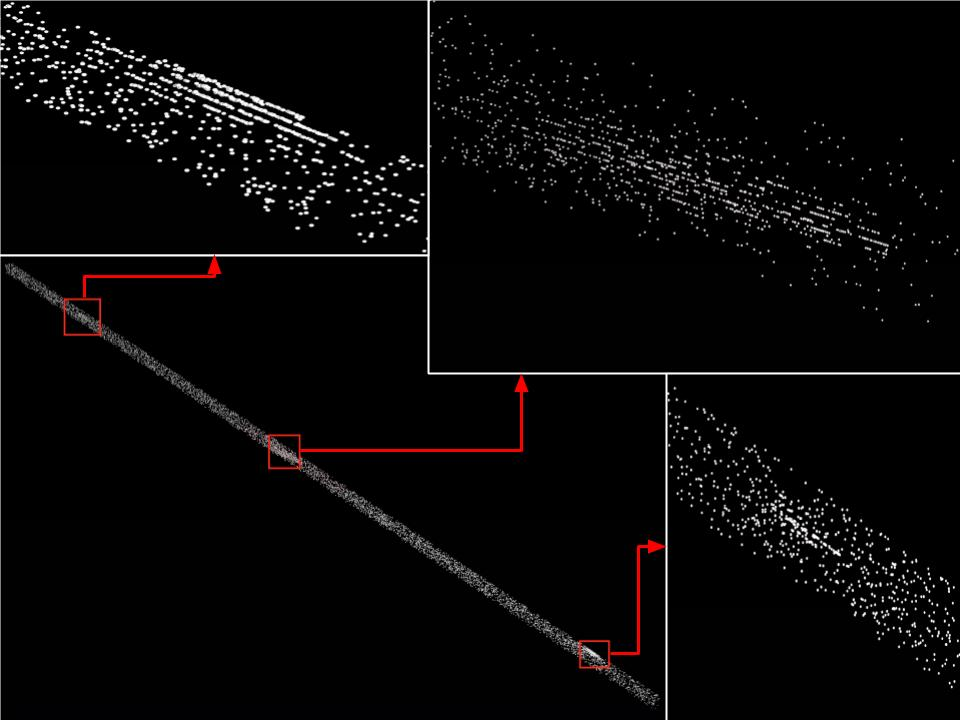
\includegraphics[width=\textwidth, height=10cm]{g_615.jpg}
    \caption{Point Cloud of the Largest Event Timeslice}
    \label{fig:g_615}
\end{figure}


Figure \ref{fig:g_615} shows a timeslice that contained the highest number of event hits. The point cloud has three event regions highlighted in red that are very hard to identify. These regions were visualised under a highly zoomed perspective using MeshLab \footnote{https://www.meshlab.net/\#description} and shows very minimal differences between event hits and the surrounding noise \cite{LocalChapterEvents:ItalChap:ItalianChapConf2008:129-136}. Figure \ref{fig:g_0} on the other hand shows a point cloud of the timeslice with the highest number of noise. Based on the observed point clouds, it was decided that the data could be enhanced by elimination of points. Certain noise hits could be identified as outliers and removed in order for clusters of event hits to stand out more. 

\begin{figure}[ht!]
    \centering 
    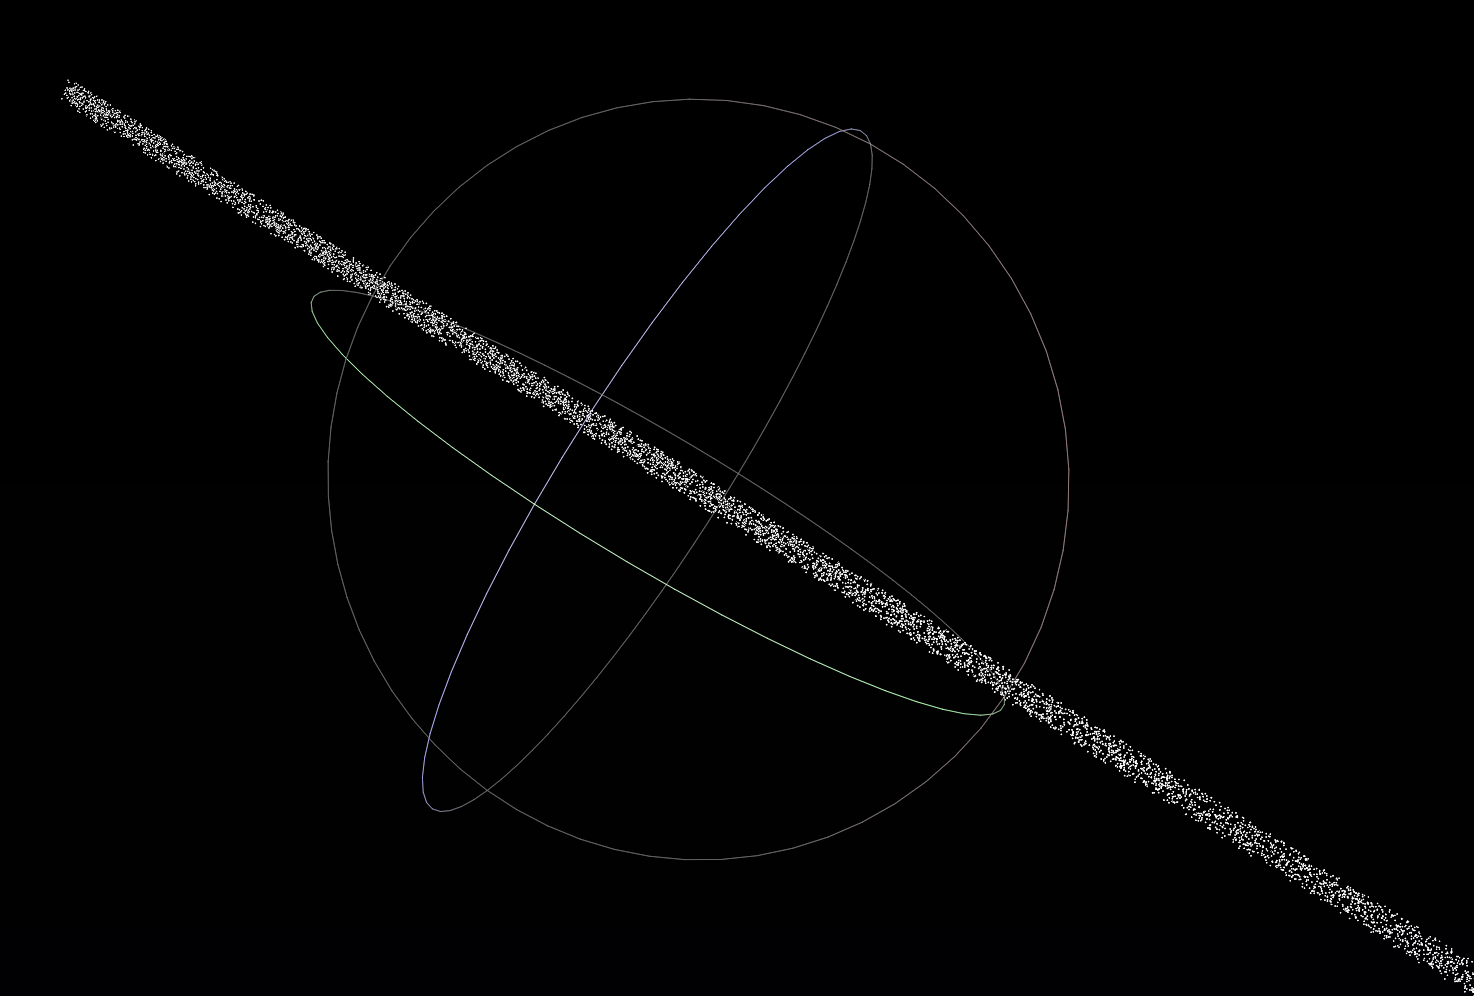
\includegraphics[width=\textwidth, height=6cm]{group_0.png}
    \caption{Point Cloud of the Largest Noise Timeslice}
    \label{fig:g_0}
\end{figure}

Removing outliers from point clouds are a common task and often manually removed using point cloud processing software \cite{LocalChapterEvents:ItalChap:ItalianChapConf2008:129-136}. Surface fitting-based methods are a popular means of outlier removal. Here, a triangulated surface gets generated and criterion such as Moving Least Squares with Lagrangian operators are used to identify "rough" features from irregular regions \cite{lipman2007parameterization}. Discontinuous operators-based method is another reliable technique whereby regions of points are detected using density depth maps and removed based on visibility conflict \cite{qi2016hedged}. All methods described have the advantage of being conceptually accurate \cite{ning2018efficient}. Discontinuous operators based methods however work only on specific outliers and are inapplicable elsewhere \cite{qi2016hedged}. Surface based methods can work well on logical shapes but may not make sense for irregular, unknown shapes. They can also be very time consuming due to the typically large size of point clouds \cite{lipman2007parameterization, kobbelt2004survey}. This thesis required a technique that could work well on irregular point clouds. Moreover, the focus was on providing fast processing, rather than precise outlier detection. This is because the transformed point clouds would ultimately be passed onto PointNet that should perform additional computations to differentiate between the two classes. Based on these requirements, a simple radius-based outlier detection method was finalised \cite{ning2018efficient}. 

\begin{figure}[ht!]
    \centering 
    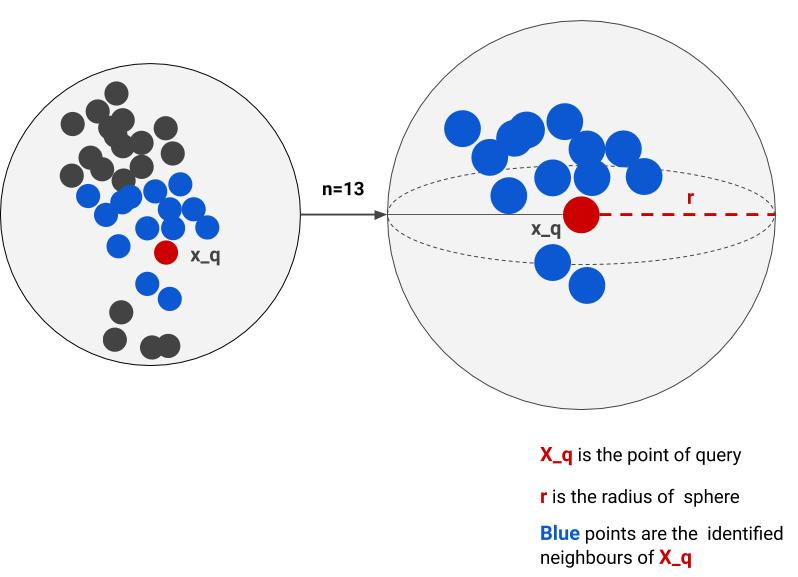
\includegraphics[width=0.7\textwidth,height=6cm, keepaspectratio]{p1_rbof.jpg}
    \caption{Demonstration of the Principle of Radius-Based Outlier Removal on A Set of Points}
    \label{fig:p1_rbof}
\end{figure} 

The principle of radius-based outlier filter (RBOF) is that if the number of points in the sphere of radius \texttt{r} centred at the query point \texttt{X\_q} is lower than a threshold \texttt{n}, then \texttt{X\_q} will be marked as an outlier and removed \cite{li2019overlapping}. Figure \ref{fig:p1_rbof} explains the concept of radius-based outlier removal where the red point (\texttt{X\_q}) is the point of interest. The number of neighbours is specified to be 13. Based on a specified radius \texttt{r}, there are 13 blue points that lie within the sphere of \texttt{X\_q}. Thus, \texttt{X\_q} is identified as outlier. Visual analysis of point clouds such as in Figures \ref{fig:g_615} and \ref{fig:g_0} helped determine that noise timeslices had roughly evenly spaced points. Therefore, the goal of RBOF was that fewer outliers would be detected and removed. Event timeslices however showed clustering of points, so here, the algorithm would detect and remove more outliers, especially the noise hits around the event clusters. 

% Feature Engineering process
\begin{figure}[ht!]
    \centering 
    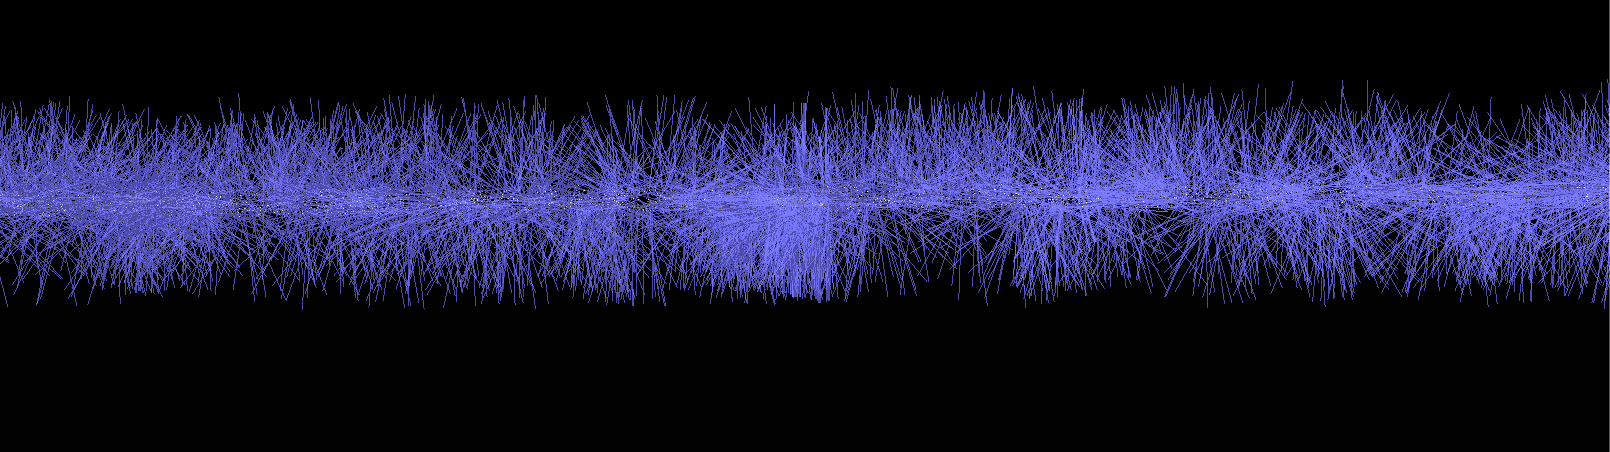
\includegraphics[width=\textwidth, height=4cm,keepaspectratio]{p1_normals_10.png}
    \caption{Normals computed for a Timeslice with Nearest Neighbours Specified as 10}
    \label{fig:p1_normals_10}
\end{figure}

Open3D\footnote{http://www.open3d.org/} was used to identify outliers and perform feature engineering. First, all \texttt{.xyz} files from each class were transformed from an array of 3D coordinates to an \texttt{o3d.geometry.PointCloud} geometry. Next, normals were computed for each point because surface reconstruction based 3D meshing requires normals of the point cloud \cite{mitra2003estimating}. The number of neighbours used to estimate normals was set to \texttt{300}, due to the large number of points per point cloud. 


Figure \ref{fig:p1_normals_10} shows the normals for a timeslice with the largest number of event hits, when computed with the default \texttt{10} neighbours. The purple markers indicate the direction of the normal. Ideally, the markers for all points must face in the same direction, which is not the case in Figure \ref{fig:p1_normals_10}. Figure \ref{fig:p1_normals} shows the same timeslice, recomputed with \texttt{300} nearest neighbours. The markers now approximately point in the same direction. The highlighted regions in the figure correspond to event hits and show interesting behaviour. The normals computed at these locations all point at different directions. 

\begin{figure}[ht!]
    \centering 
    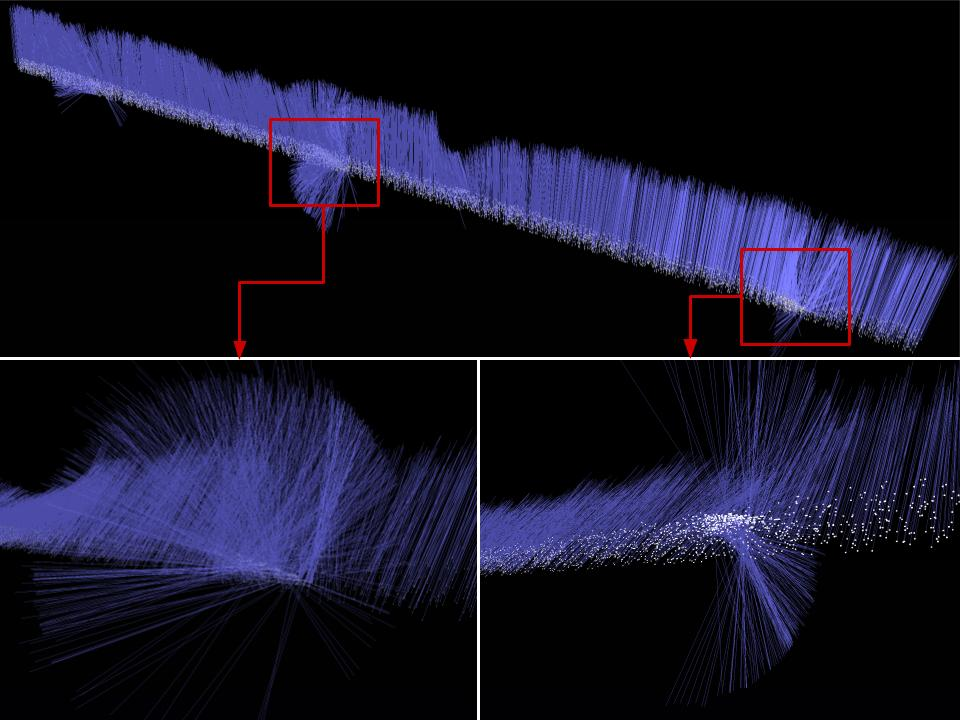
\includegraphics[width=\textwidth,keepaspectratio]{p1_normals.jpg}
    \caption{Normals computed for a Timeslice with Nearest Neighbours Specified as 300}
    \label{fig:p1_normals}
\end{figure}

With the point clouds normalised, the radius-based outlier detection was finally performed. The minimum amount of points that the sphere should contain (\texttt{nb\_points}) was left as the default value of \texttt{32} neighbours. The \texttt{radius} of the sphere that would be used for counting the neighbours was set to vary for each point cloud because of their irregular shapes and densities. A fixed radius value would not generalise well and produce inaccurate results. In order to identify a suitable radius, the nearest neighbour algorithm was used to compute the distance from a point to its nearest neighbour in the point cloud \cite{cui2018flexible}. Once an array of all the distances were obtained, they were averaged and multiplied by a factor of 3.6 to account for scaling \cite{zhou2018open3d}.

\begin{figure} [ht!]
    \centering
    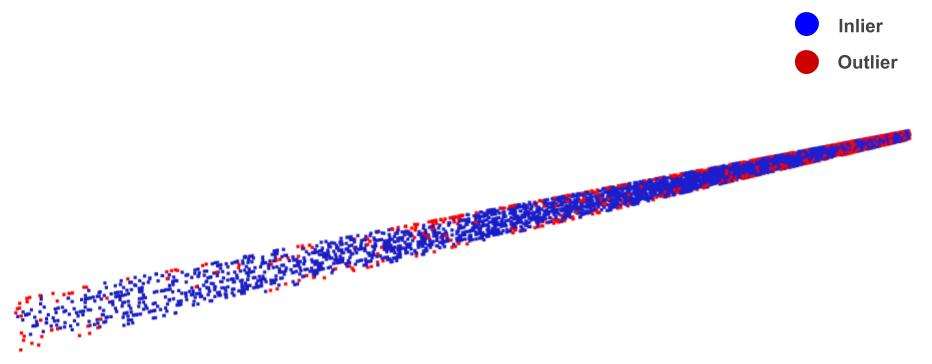
\includegraphics[width=0.7\textwidth, height=4cm]{p1_outlier_noise}
    \caption{Result of Radius-Based Outlier Detection on Timeslice with Only Noise}
    \label{fig:p1_outlier_noise}
\end{figure}

Figure \ref{fig:p1_outlier_noise} shows the result of applying the outlier removal on a timeslice with only noise. The algorithm identified inliers in blue and outliers in red. 

\begin{figure}[htb!]   
\centering
\subfloat[Noise Timeslice Before and After Outlier Removal]{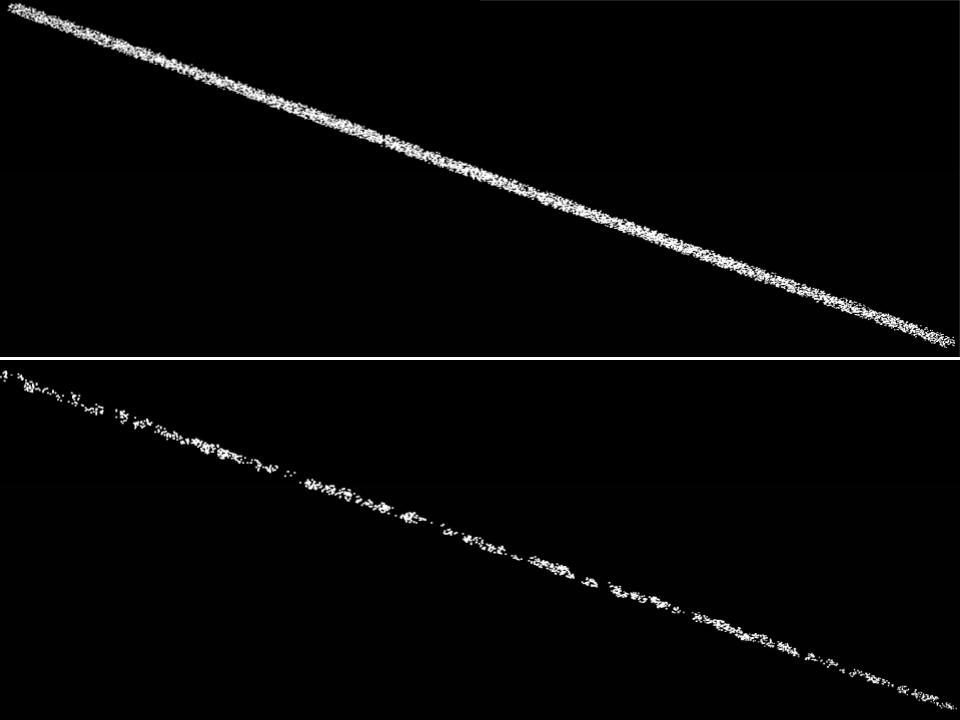
\includegraphics[width=0.49\textwidth,height=5cm]{p1_noise_after_outlier_removal.jpg}\label{fig:p1_noise_after_outlier}}
\hspace{0.1cm}
\subfloat[Event Hits Timeslice Before (Top) and After (Bottom) Outlier Removal]{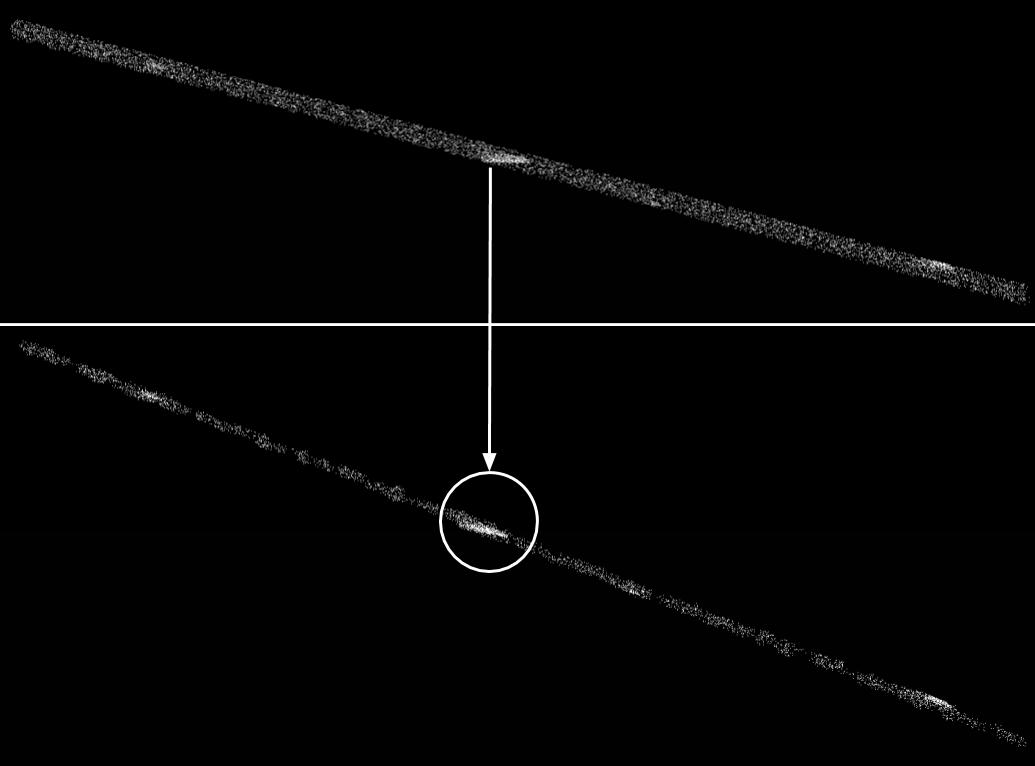
\includegraphics[width=0.49\textwidth,height=5cm, keepaspectratio]{p1_hits_after_outlier_removal.jpg}\label{fig:p1_hits_after_outlier}}
\caption[]{Noise and Event Hits Timeslices Before (Top) and After (Bottom) Radius-Based Outlier Detection}
\label{fig:before_after_outlier}
\end{figure}

Figure \ref{fig:before_after_outlier} shows an example of a noise and event hits timeslices both before and after removal of outliers. As expected, the RBOF found a higher incidence of outliers in the event timeslice. The resulting point cloud is more simplified with the event hit clusters intact, as highlighted in Figure \ref{fig:p1_hits_after_outlier}. Similarly, Figures \ref{fig:p1_outlier_615} and \ref{fig:p1_outlier_hit} shows the result of the algorithm on timeslices with event hits. As expected, event timeslices show higher number of outliers due to the presence of event clusters.

\begin{figure}[htb!]   
\centering
\subfloat[Timeslice with Highest Event Hits]{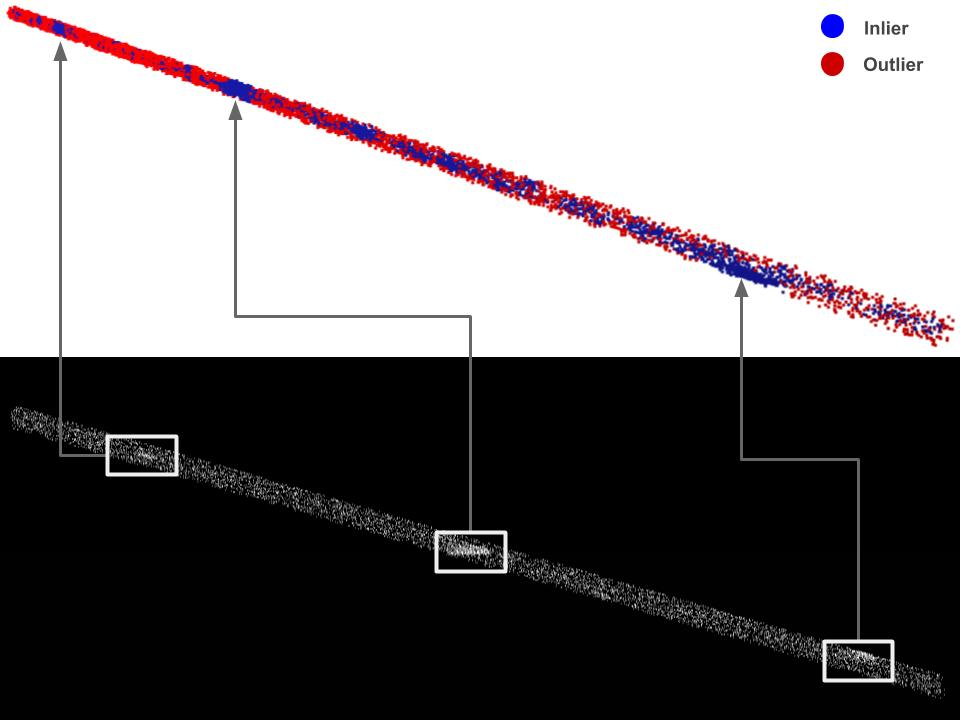
\includegraphics[width=\textwidth,keepaspectratio]{p1_outlier_615}\label{fig:p1_outlier_615}}

\subfloat[Another Event Hits Timeslice]{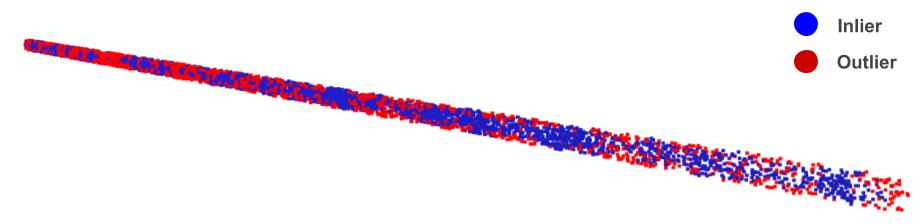
\includegraphics[width=\textwidth, height=3cm]{p1_outlier_hit}\label{fig:p1_outlier_hit}}
\caption[]{Result of Radius-Based Outlier Detection On Different Event Timeslices}
\label{fig:p1_outlier_removal}
\end{figure}

\section{3D Mesh Generation}
With the feature engineering completed, \texttt{.xyz} files were converted to 3D meshes. Meshes are a collection of geometric properties - vertices, faces and edges that describe a 3D object \cite{kim2006complete}. There are several algorithms that can convert 3D coordinates to meshes but two of the most popular algorithms were considered and evaluated \cite{kim2006complete}.

\textbf{Ball Pivoting Algorithm (BPA)} ``rolls" a virtual ball across the point cloud ``surface". It forms a triangle from the three nearest points and then rolls along that triangle to another set of three points where it forms a new triangle \cite{bernardini1999ball}. In this manner, the algorithm continues until all points are converted to a mesh. BPA requires the radius of the ball to be specified such that it is slightly larger than the average space between points \cite{bernardini1999ball}. For this thesis, using an average radius value would cause problems in the event hit clusters as the distance between points in those regions may be less than the size of the ball. This would lead the ball to roll over those points and ignore them. Given the irregular, unknown symmetry with sets of close points in event clusters, it was likely that BPA would miss the details that could indicate presence of event hits. 

\begin{figure}[ht!]   
\centering
\subfloat[Event Timeslice: Highlighted Area Corresponds to Event Hits Cluster]{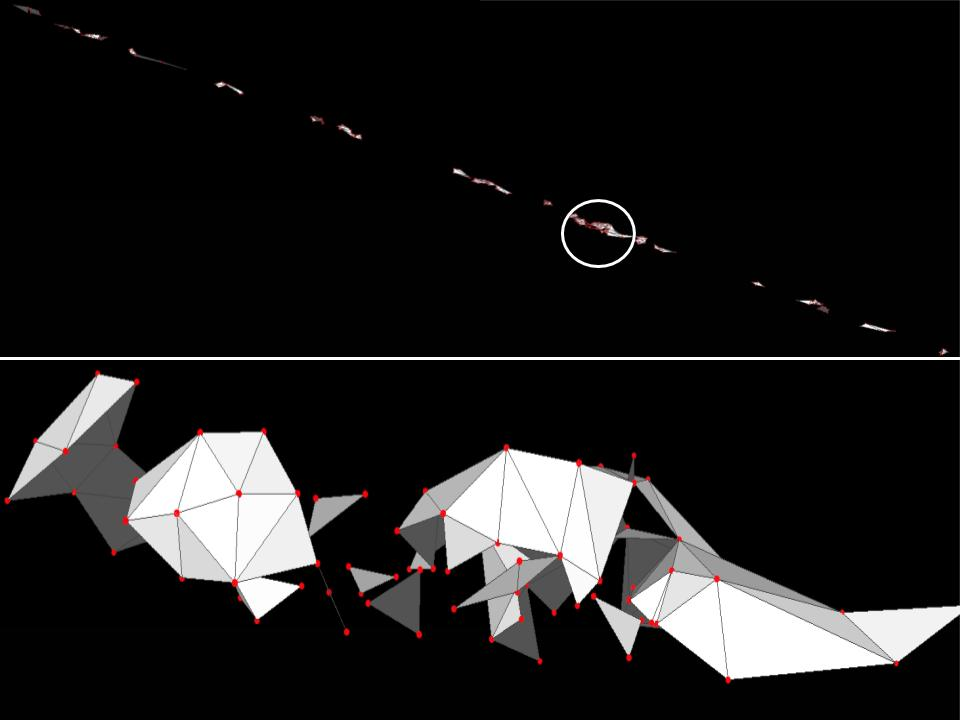
\includegraphics[width=0.49\textwidth, keepaspectratio]{p2_hits_bpa}\label{fig:p2_hits_bpa}}
\hspace{0.01cm}
\subfloat[Noise Timeslice]{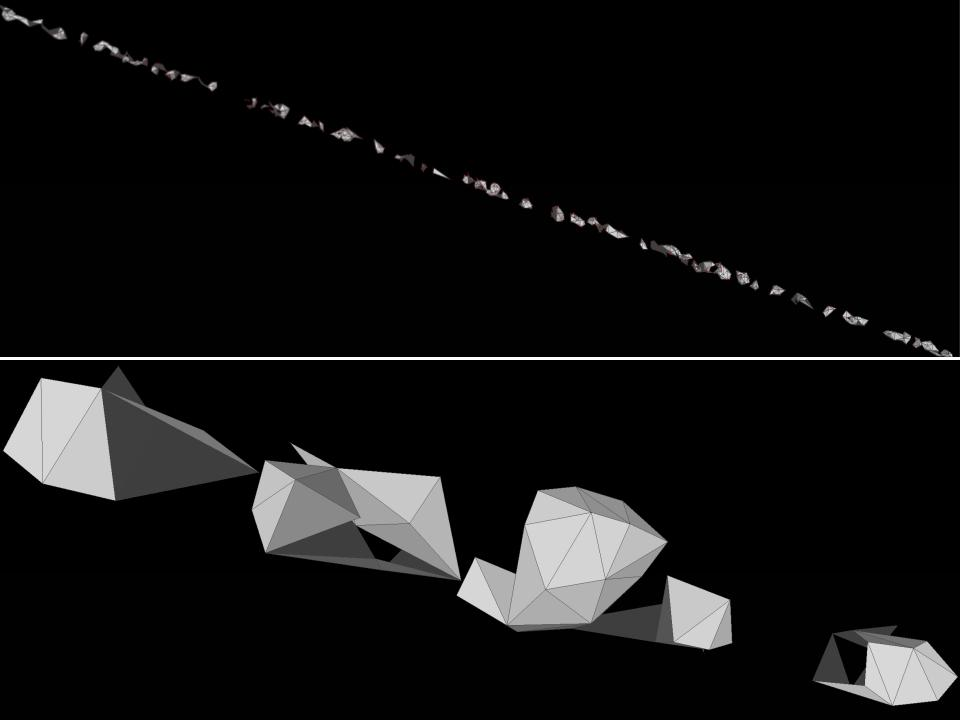
\includegraphics[width=0.49\textwidth, keepaspectratio]{p2_noise_bpa}\label{fig:p2_noise_bpa}}
\caption[]{Noise and Event Timeslices After Applying Ball Pivoting Algorithm}
\label{fig:p2_bpa}
\end{figure}

Figure \ref{fig:p2_bpa} shows the transformed point clouds after applying BPA. Figure \ref{fig:p2_hits_bpa} shows an events timeslice where event hits (in red) are overlaid with the corresponding 3D mesh for comparison. The region in focus shows an event cluster. The algorithm rolled over and missed several points, leaving gaps in the mesh. On the other hand, Figure \ref{fig:p2_noise_bpa} shows the effect of BPA on a noise timeslice. Due to the generally evenly spaced nature of noise, the algorithm was able to capture most points. However, the two meshes don't show significant differences between each other since the event clusters are not particularly enhanced. It indicated that BPA would not be sufficient for the PointNet to learn. 


% \Poisson
\textbf{Poisson Surface Reconstruction} is an implicit meshing algorithm by Kazhdan et al. (2006) that envelops points in a smooth "cloth". It tries to fit a surface from the original point set by creating an entirely new point set representing an iso-surface linked to the normals \cite{kazhdan2006poisson}. As it tries to create a watertight surface, it seemed a more promising solution for the detailed event regions. Poisson Surface Reconstruction required several parameters for the octree that is used for the reconstruction \cite{kazhdan2006poisson} - depth, scale and fit. The octree \textit{depth} specifies the level of detail of re-construction and is the most significant parameter. The \textit{scale} describes the ratio between the diameter of the cube used for reconstruction and the diameter of the samples’ bounding cube. \textit{fit} lets the re-constructor use linear or non-linear interpolation to estimate the positions of iso-vertices \cite{kazhdan2006poisson}.

\begin{figure}[ht!]   
\centering
\subfloat[Event Timeslice: Highlighted Area Corresponds to Event Hits Cluster]{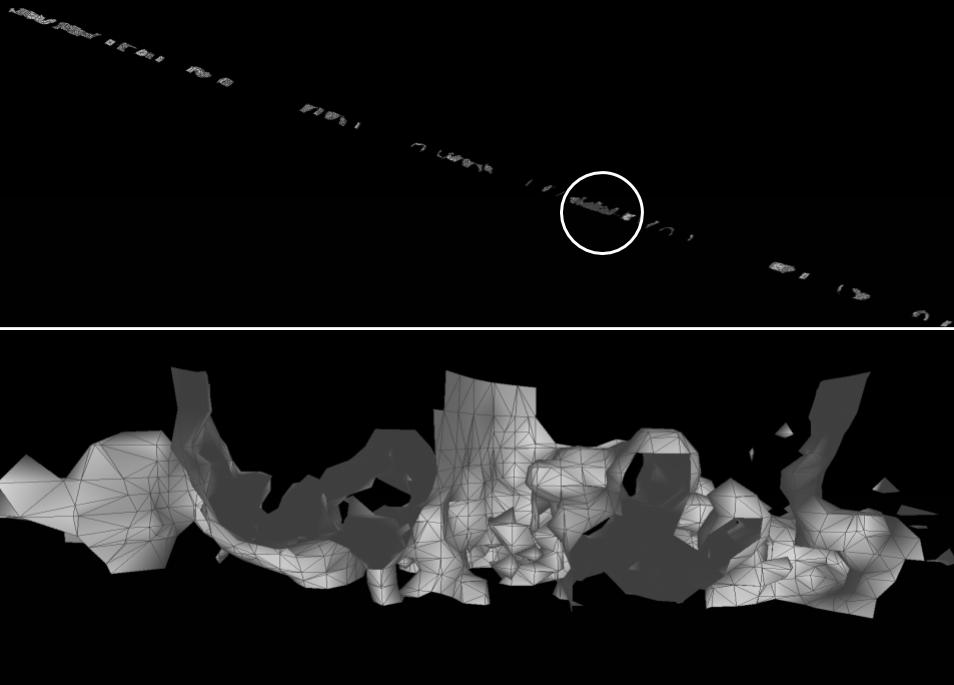
\includegraphics[width=0.49\textwidth, keepaspectratio]{p2_hits_sp}\label{fig:p2_hits_sp}}
\hspace{0.01cm}
\subfloat[Noise Timeslice: Highlighted Area Corresponds to Noisy Artefact ]{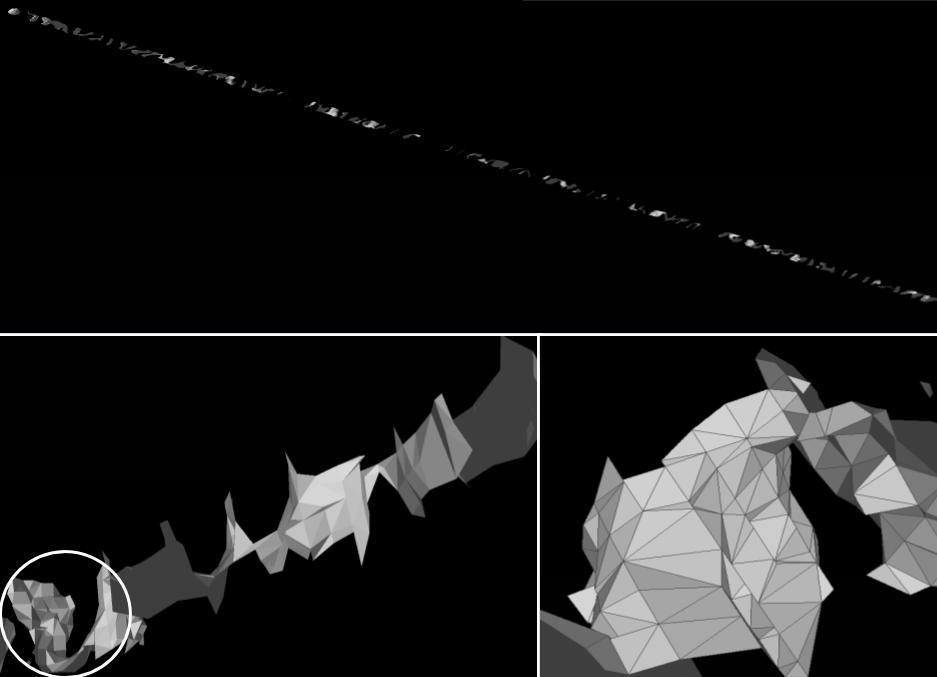
\includegraphics[width=0.49\textwidth, keepaspectratio]{p2_noise_sp}\label{fig:p2_noise_sp}}
\caption[]{Noise and Event Timeslices After Applying Surface Poisson Reconstruction}
\label{fig:p2_sp}
\end{figure}

Default parameters of depth \texttt{10}, octree scale \texttt{1.1} and \texttt{non-linear} interpolation were used  \cite{LocalChapterEvents:ItalChap:ItalianChapConf2008:129-136}. Figure \ref{fig:p2_sp} shows the same timeslices as before, rendered with Poisson Surface Reconstruction. Poisson Surface Reconstruction shows a more detailed mesh for the event hits region in the event timeslice in Figure \ref{fig:p2_hits_sp}. Figure \ref{fig:p2_noise_sp} shows the algorithm rendered on the noise timeslice. The surface is more or less flat and even. However, the Reconstruction algorithm produced some noisy artefacts, as highlighted in the image.

Based on the difference in mesh detail between BPA and Poisson Surface Reconstruction, Poisson Surface Reconstruction did a better job of capturing event hits. The noisy artefacts generated in noise timeslices could pose a problem, however PointNet should be able to better distinguish between the two classes based on other features. 


\section{PointNet}
PointNet was implemented in PyTorch \footnote{https://pytorch.org/} and a few modifications were made to work with the KM3NeT Data. Input batch (training examples) for PointNet can be 1D or 2D convolutions \cite{qi2017pointnet}. A convolution involves the application of a filter to the input that results in an activation function \cite{goodfellow2016convolutional}. For the thesis, 1D convolutions were used as it can help reduce dimensions and computational costs \cite{lin2013network}. In this case, the 1D convolution was the Multi-Layer Perceptron (MLP) with shared weights and kernel of size 1.

Pooling layers allow for down-sampling feature maps by means of a summary \cite{goodfellow2016convolutional}. Two common pooling methods include max pooling which summarises the most activated presence of a feature; and average pooling which summarises the average presence of a feature \cite{goodfellow2016convolutional}. Instead of using a global max pool function suggested in the paper by Qi et al. (2017), an average pool function was applied to the transformed features \cite{qi2017pointnet}. This was done because max pool was found to cause some overfitting to the KM3NeT data.

The paper by Qi et al. (2017), used Cross Entropy Loss, a typical loss function for classification \cite{qi2017pointnet}. However, thesis experiments showed that the network learned better with the negative log-likelihood (NLL) loss. As the NLL loss requires log probabilities of each class, the Log Sigmoid activation was also applied to the output layer \cite{paszke2019pytorch}. The remainder of the architecture was left unchanged. 

\subsection{PointNet Transformations}
\begin{figure}[ht!]   
\centering
\subfloat[Events Timeslice With Vertices from Mesh]{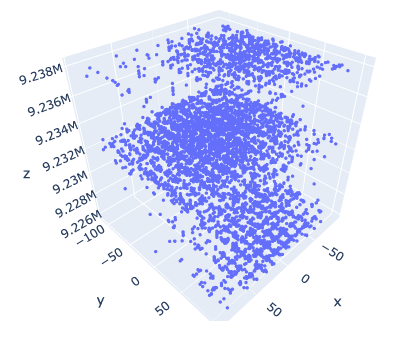
\includegraphics[width=0.49\textwidth,height=6cm,]{hits_vertices.png}\label{fig:hits_v}}
\hspace{0.01cm}
\subfloat[Noise Timeslice With Vertices from Mesh]{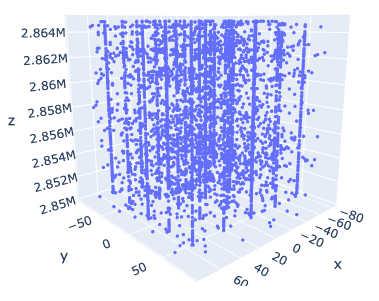
\includegraphics[width=0.49\textwidth,height=6cm]{noise_vertices.png}\label{fig:noise_v}}
\caption[]{Noise and Event Timeslices With Non-Uniform Distribution of Mesh Vertices}
\label{fig:vertices}
\end{figure}

Qi et al. (2017) stated three requirements for training point clouds with PointNet (Section \ref{sec:concepts}). Point clouds should be unordered and PointNet has to be invariant to permutations of the input set. Next, the network must be invariant to rigid transformations. Finally, the network should also capture interactions among points \cite{qi2017pointnet}. The thesis implemented the recommended transformations to the input point clouds during training and testing to ensure conformity of data to the above requirements \cite{qi2017pointnet}.

Points are not uniformly distributed across the 3D object’s surface, hindering PointNet's ability to classify them. For example, Figure \ref{fig:vertices} shows non-uniformity in the distribution of vertices from the meshes for both noise and event class. 

\begin{figure}[ht!]   
\centering
\subfloat[Event Hits Timeslice Sampled with 1024 Points]{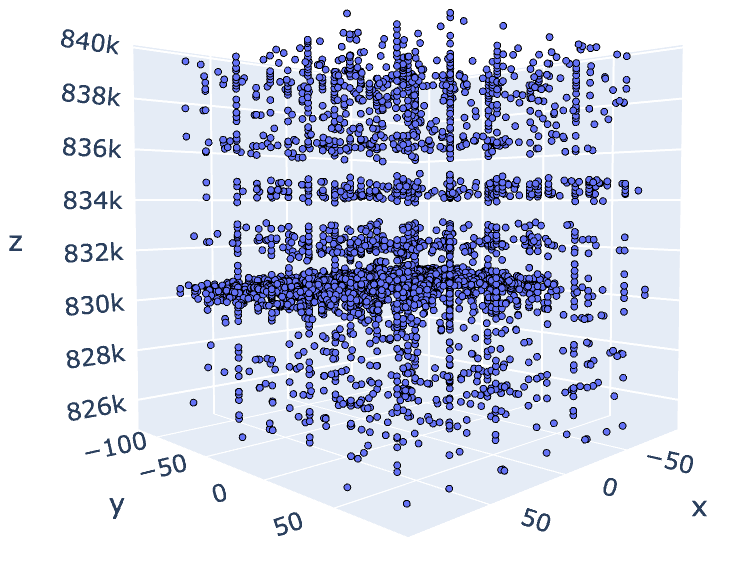
\includegraphics[width=0.49\textwidth,height=7cm, keepaspectratio]{hits_1024_sampled.png}\label{fig:hits_1024}}
\hspace{0.01cm}
\subfloat[Event Hits Timeslice Sampled with 8192 Points]{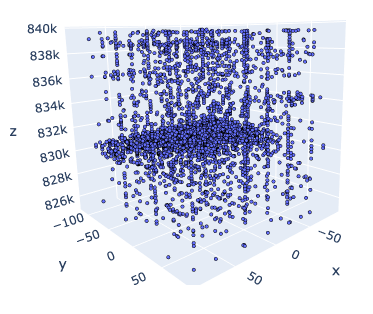
\includegraphics[width=0.49\textwidth,height=5.5cm]{hits_8192_sampled.png}\label{fig:hits_8192}}
\hspace{0.01cm}

\subfloat[Noise Timeslice Sampled with 1024 Points]{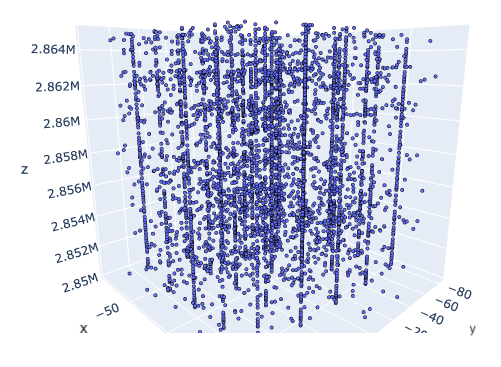
\includegraphics[width=0.49\textwidth, height=7cm, keepaspectratio]{noise_1024_sampled.png}\label{fig:noise_1024}}
\subfloat[Noise Timeslice Sampled with 8192 Points]{\includegraphics[width=0.49\textwidth,height=7cm, keepaspectratio]{noise_1024_sampled.png}\label{fig:noise_8192}}
\caption[]{An Example of Noise and Event Timeslices With Different Levels of Sampling}
\label{fig:sampled}
\end{figure}

PointNet also requires a fixed number of points to be sampled per point cloud \cite{qi2017pointnet}. While Qi et al. (2017) uniformly sampled 1024 points on mesh faces, it was found that this number was not sufficient for the KM3NeT Data.  Figure \ref{fig:sampled} shows both classes of point clouds randomly sampled with 1024 points and then with 8192 points (points have to be in multiples of 1024). While noise timeslices were relatively unaffected, event timeslices showed better structure with greater points. The thesis sampled one point per chosen face. Additionally, as faces had different areas, a probability was assigned to choose a particular face proportional to its area. That is, faces with higher area had higher probability of being chosen as it represented more of the surface \cite{qi2017pointnet}. In this manner, a total of 8192 point were sampled per point cloud.

\begin{figure}[ht!]   
\centering
\subfloat[Event Hits Timeslice]{\includegraphics[width=0.49\textwidth, height=6cm, keepaspectratio]{hits_normalised.png}\label{fig:hits_norm}}
\subfloat[Noise Timeslice]{\includegraphics[width=0.49\textwidth, height=6cm,keepaspectratio]{noise_normalised.png}\label{fig:noise_norm}}
\caption[]{An Example of Noise and Events Timeslice After Normalisation}
\label{fig:normalised}
\end{figure}

Point clouds in the KM3NeT dataset have different sizes and are often placed in different parts of the coordinate system. Qi et al. (2017) normalised point clouds along a unit sphere \cite{qi2017pointnet}. The thesis also applied similar translations. Point cloud were translated to the origin by subtracting the mean from all its points, and then normalising them into a unit sphere \cite{qi2017pointnet}. Figure \ref{fig:normalised} shows the effect of this normalisation for both classes.

Qi et al. (2017) also augmented point clouds during training by adding jitter and randomly rotating the objects \cite{qi2017pointnet}. Therefore, the event and noise point clouds were randomly rotated around the Z-axis. Jitter via Gaussian noise was also added with \texttt{0} mean and \texttt{0.02} standard deviation \cite{qi2017pointnet}. Figure \ref{fig:augmented} shows the effect of these augmentations for both classes. 

\begin{figure}[ht!]   
\centering
\subfloat[Event Hits Timeslice]{\includegraphics[width=0.49\textwidth, height=6cm, keepaspectratio]{hits_augmented.png}\label{fig:hits_aug}}
\hspace{0.01cm}
\subfloat[Noise Timeslice]{\includegraphics[width=0.49\textwidth,height=6cm, keepaspectratio]{noise_augmented.png}\label{fig:noise_aug}}
\caption[]{An Example of Noise and Event Timeslices After Jitter and Random Rotation}
\label{fig:augmented}
\end{figure}

The application of the recommended augmentations resulted two fairly distinct point clouds and was considered effective. The noise timeslice formed a dense block while the events timeslice formed a collection of points with gaps in between.

Figure \ref{fig:core_pipeline} shows an overview of the pipeline that was used for each of the three datasets - \texttt{(x y time)}, \texttt{(x z time)} and \texttt{(y z time)}. First, 3D coordinates were generated and separated into two classes. Feature engineering using radius-based outlier filter eliminated several points, enhancing event clusters. Surface Poisson Reconstruction was applied to convert the coordinates to 3D meshes. PointNet transformation functions were also added to enhance the point clouds on the fly during training and testing.

\begin{figure}[ht!]
    \centering
    \includegraphics[trim={5.25cm 0 5.5cm 0}, clip, width=\linewidth,keepaspectratio]{core_pipeline}
    \caption{KM3NeT Pipeline Components}
    \label{fig:core_pipeline}
\end{figure}

\let\cleardoublepage\clearpage



\chapter{Evaluation Methodology}
\label{sec:evaluation}
\ifpdf
    \graphicspath{{6_evaluation/figures/PNG/}{6_evaluation/figures/PDF/}{6_evaluation/figures/}}
\else
    \graphicspath{{6_evaluation/figures/EPS/}{6_evaluation/figures/}}
\fi

The selected timeslices had between 500 to 1692 event hits to capture a variety of event sizes for training. Figure \ref{fig:7_tree} shows the directory structure for the dataset. Timeslices were organised by classes and separated into individual \texttt{training} and \texttt{testing} folders as required by PointNet.

\begin{figure}[ht!]
    \centering
    \includegraphics[width=0.4\textwidth, height=5.5cm, keepaspectratio]{tree}
    \caption{Required Directory Structure for PointNet}
    \label{fig:7_tree}
\end{figure}

An 80-20 train-test split was used to randomly select 80\% of the files under each class for training and 20\% for testing. No validation set was required because there was no need to choose an appropriate model from rivalling approaches \cite{dixon2017deep, james2013introduction}. This chapter discusses the preparation of the training and testing data, along with two chosen edge cases. The chapter also describes the ensemble methodology used for obtaining final predictions and remarks on the use of L1 trigger on the dataset for comparison against PointNet.

\section{Training and Testing Data}
\label{sec:eval_train_test_data}
160 timeslices were selected for each class as training data. Both classes had meshes with approximately 4800 vertices on average, and 8500 triangles. A total of 40 timeslices were selected as testing data for each class. Both classes had meshes with approximately 4800 vertices on average and 7500 triangles. The testing data represented much of what the detector would gather in real world, and send to the pipeline for processing. However, two additional edge cases were chosen to evaluate the extent of the model's learning capacity. Most event timeslices have around 700 event hits on average. Therefore, a timeslice with 100 event hits and 6796 noise hits was selected. As an extreme case, a group with 39 event hits and 6645 noise hits was selected.

\begin{figure}[ht!]   
\centering
\subfloat[3D Mesh of Timeslice with 100 Event Hits]{\includegraphics[width=0.49\textwidth, height=6cm, keepaspectratio]{1063.png}\label{fig:1063-mesh}}

\subfloat[Typical Example of Timeslice with Event Hits]{\includegraphics[width=0.49\textwidth,height=3.7cm]{615.png}\label{fig:615-mesh}}
\hspace{0.01cm}
\subfloat[Typical Example of Timeslice with Noise]{\includegraphics[width=0.49\textwidth,height=6cm, keepaspectratio]{noise.png}\label{fig:noise-mesh}}
\caption[]{Edge Case: Comparison of Mesh Detail for Timeslices with Low Event Hits}
\label{fig:1063}
\end{figure}

Figure \ref{fig:1063-mesh} shows the detail captured by the mesh for a processed point cloud with 100 event hits.
Figure \ref{fig:615-mesh} on the other hand is an example of a typical event cluster rendered with details and rounded surfaces. Figure \ref{fig:noise-mesh} is an example of a typical noise region, rendered as smoother surfaces by Surface Poisson Reconstruction. Figure \ref{fig:1063-mesh} resembles the noise point cloud in Figure \ref{fig:noise-mesh} with smooth surfaces. This indicated that the event hits details were lost in conversion and PointNet may not be able to classify it as an event timeslice. 

Similarly, Figure \ref{fig:5686} shows another example of a point cloud with 39 event hits. The mesh representation contains very few distinguishing features and flat surfaces, unlike a typical event cluster mesh (Figure \ref{fig:615-mesh}). Since the event cluster resembled the mesh representing noise hits, it was likely that PointNet would not be able to classify it as an events class.

\begin{figure}[ht!]
    \centering
    \includegraphics[trim={1cm 1cm 0.5cm 0.5cm}, clip,width=0.7\linewidth,keepaspectratio]{5686.png}
    \caption{3D Mesh of Timeslice with 39 Event Hits}
    \label{fig:5686}
\end{figure}

\section{Model Specifications}
The model was first run for \texttt{200} epochs to find the optimal training epoch value. Figure \ref{fig:epochs} shows that the loss settled around 100 to 120 epochs. Therefore, the rest of the experiments were conducted for \texttt{120} epochs. The loss was found to be between \texttt{0.008} and \texttt{0.003} during training and considered sufficient for the thesis. 

\begin{figure}[ht!]
    \centering
    \includegraphics[trim={0 0 0 0.3cm}, clip, width=0.7\linewidth,keepaspectratio]{epochs}
    \caption{Loss Plotted for 200 Training Epochs}
    \label{fig:epochs}
\end{figure}

Model parameters were experimented to obtain optimal performance, but it was noted that the default parameters in the paper by Qi et al. (2017) were best suited for the dataset \cite{qi2017pointnet} (Appendix \ref{appendix-layers}). Table \ref{tab:model_parameters} shows the parameters used for training. For each batch, the model was evaluated on the testing data to obtain a signal about the model's ability to generalise. The dataset was trained with PyTorch using Google Colab NVIDIA Tesla K80 GPU and on ViltStift AMD MI50 GPUs for approximately 3.5 hours.

\begin{table} [ht!]
    \centering
    \begin{tabular}{l c}
    \hline
        regularisation loss with weight & 0.001  \\
        Initial Learning Rate & 0.001 \\
        Dropout probability & 0.3 \\
        Batch Size Training & 32 \\
        Batch Size Testing & 64 \\
        Epochs & 120\\
    \hline
    \end{tabular}
    \caption{Final Model Parameters Used for Training on KM3NeT Data}
    \label{tab:model_parameters}
\end{table}

 
\section{Ensemble Methods for Results}
As \texttt{x, y, z,} and \texttt{time} variables were split into three permutations of (\texttt{x, y, time}), (\texttt{x, z, time}) and (\texttt{ y, z, time}), each dataset was trained separately. The results from each of these datasets were then combined using majority voting ensemble techniques \cite{goodfellow2016convolutional}. Voting ensembles were selected as a suitable methodology for two main reasons. First, while there were three datasets, they represented the same information, except in slightly different manner. Majority voting ensembles place equal value on the models being combined to make predictions which was relevant in this case \cite{bhowan2012evolving}. Second, a voting ensemble is considered appropriate when no single model performs comparatively worse or better than the others \cite{bhowan2012evolving}. Results showed that two of the three models were quite similar in performance.

Two voting ensemble techniques were used to generate the final predictions - hard voting and soft voting. A hard voting ensemble sums the votes for class labels from all models and presents the class with the most vote as the final prediction \cite{witten2002data}. A soft voting ensemble sums the predicted probabilities for class labels and presents the label with the highest sum probability \cite{witten2002data}. A soft voting ensemble additionally requires a probability threshold to finalise the label as positive. A high threshold of 90\% was used due to the physics requirement of minimising false positives and correctly classifying event timeslices as much as possible.

The existing L1 trigger (Section \ref{sec:intro-trigger}) was also applied on the dataset. The results from the L1 trigger were contrasted against PointNet to identify if any improvements could be noted. The L1 trigger is known to save noise timeslices as relevant, so PointNet would have to perform better in that instance. The training and testing data was therefore prepared to ensure that a good range of event sizes were covered. Further, two edge cases for event timeslices were also prepared to establish the extent of the network's learning capacity. Majority voting ensemble was seen as a robust, simple ensemble technique and used to obtain final predictions.



\chapter{Classification Results}
\label{sec:results}

\ifpdf
    \graphicspath{{7_results/figures/PNG/}{7_results/figures/PDF/}{7_results/figures/}}
\else
    \graphicspath{{7_results/figures/EPS/}{7_results/figures/}}
\fi

Accuracy score is typically used to identify optimal models, however as a metric it is often not interpretable and discriminative \cite{hossin2015review}. Moreover, an accuracy score is almost always biased towards the majority class. The goal was to ensure that timeslices with neutrinos did not get mislabelled as noise. Therefore, \textit{recall} was the most significant metric for the classification task.
Based on the highly imbalanced nature of the dataset and the physics goal, a few other metrics were also required \cite{scikit-learn}. This chapter establishes the relevant metrics selected for classification and discusses the results obtained through plots and summaries. 

\textbf{Precision} measures the percentage of results that are relevant. It is the ability of the classifier to not label a negative sample as positive \cite{scikit-learn}. Precision is given by the number of true positives (${T}_p$) over the number of true positives (${T}_p$) plus the number of false positives (${F}_p$):
    \[
        P = \frac{{T}_p}{{T}_p + {F}_p}
    \]
    
\textbf{Recall} refers to the percentage of total relevant results correctly classified, and is the ability of the classifier to find all positive samples \cite{scikit-learn}. It is given by the number of true positives (${T}_p$) over the number of true positives (${T}_p$)  plus the number of false negatives (${F}_n$):
    \[
        R = \frac{{T}_p}{{T}_p + {F}_n}
    \]

\textbf{F1 Score} is a weighted harmonic mean of the precision and recall \cite{scikit-learn}. It is given by:
    \[
        F1 = 2 \times \frac{P \times R}{P + R}
    \]

\textbf{Receiver Operating Characteristic (ROC) Curves} depict the trade-off between true positive rate and false positive rate for different probability thresholds \cite{scikit-learn}.
 
\textbf{Precision-Recall (PR) Curve} shows the trade-off between precision and recall for different thresholds \cite{scikit-learn}. A high area under the curve represents both high recall and high precision. 

\textbf{Confusion Matrix} visualises the number of true positives, false positives, true negatives and false negatives \cite{jaffery2009measuring} . 

Each of the three datasets - (\texttt{x, y, time}),  (\texttt{x, z, time}), and (\texttt{y, z, time}) were trained using the same PointNet model parameters (Table \ref{tab:model_parameters}), and their results combined using ensemble techniques. Table \ref{tab:results} shows the final classification accuracy scores for each of the three datasets and the results after applying two majority voting ensemble methods. 

\begin{table} [ht!]
    \centering
    \begin{tabular}{l c}
    \hline
        \texttt{x, y, time} & \textbf{95\% } (loss = 0.003)\\
        \texttt{x, z, time} & \textbf{90\%} (loss = 0.006)\\
        \texttt{y, z, time} & \textbf{99\%} (loss = 0.005)\\
        Ensemble 1: Hard Voting & \textbf{97\%}\\
        Ensemble 2: Soft Voting & \textbf{90\%}\\
    \hline
    \end{tabular}
    \caption{Accuracy Scores}
    \label{tab:results}
\end{table}

A classification report was generated for each dataset and the two ensembles to obtain detailed performance report on precision, recall and F1 Scores. ROC Curves and PR Curves were both plotted to compare against each other. This is because ROC curves are more appropriate for balanced classes and PR curves are better suited for imbalanced datasets. Keeping in mind the physics goal, analysis was more focused on the model's performance in (mis)classifying event timeslices (\texttt{class\_1}). 

\section{Dataset 1: \texttt{x, y, time}}

The \texttt{x, y, time} model reported a 95\% accuracy. Classification report in Table \ref{tab:xyt_classification_report} shows that the model did not mislabel any noise (\texttt{class\_0}) as event \texttt{class\_1} timeslices. Further, \textbf{90\%} of the total relevant results were correctly classified as \texttt{class\_1}. Support indicates that 40 test cases were used for each class.

\begin{table} [ht!]
    \centering
    \begin{tabular}{l c c c c}
    \hline
    \multicolumn{5}{c}{\texttt{x, y, time}} \\
    \hline
                     & precision  & recall& F1-score & support \\
        \texttt{class\_0} & 0.91  &  1.00    & 0.95 & 40\\
        \texttt{class\_1} & 1.00  &  0.90    & 0.95 & 40\\
    \hline
    \end{tabular}
    \caption{\texttt{x, y, time}: Classification Report for \texttt{class\_0} and \texttt{class\_1}}
    \label{tab:xyt_classification_report}
\end{table}

Figure \ref{fig:xyt_results} shows the relevant plots  of metrics for the dataset. The ROC curves are towards the top left of the graph and indicate a desirable, high true positive rate against the baseline performance plotted on the diagonal. Complementing the ROC, the Precision-Recall (PR) curves show a high area under the curve, indicating high precision and recall. Precision was mostly stable for increasing recall, but it fell dramatically for \texttt{class\_1} after 85\% recall. The confusion matrix shows that 4 of the 40 timeslices with event hits were incorrectly labelled as noise, but none of the noise timeslices were incorrectly labelled.
 
\begin{figure}[ht!]
    \centering
    \includegraphics[width=\textwidth,keepaspectratio]{xyt.pdf}
    \caption{\texttt{x, y, time}: Classification Plots}
    \label{fig:xyt_results}
\end{figure}

\section{Dataset 2: \texttt{x, z, time}}
\begin{table} [ht!]
    \centering
    \begin{tabular}{l c c c c}
    \hline
    \multicolumn{5}{c}{\texttt{x, z, time}} \\
    \hline
                     & precision & recall & F1-score & support \\
        \texttt{class\_0}  & 0.83 &  1.00    & 0.91 & 40\\
        \texttt{class\_1}  & 1.00 &  0.80    & 0.89 & 40\\
    \hline
    \end{tabular}
    \caption{\texttt{x, z, time}: Classification Report for \texttt{class\_0} and \texttt{class\_1}}
    \label{tab:xzt_classification_report}
\end{table}

The \texttt{x, z, time} model reported a lower accuracy of 91\%. This is because it wrongly classified a higher percent of \texttt{class\_1} samples (Table \ref{tab:xzt_classification_report}). The model was however much better at detecting noise and obtained a \textbf{perfect recall}.

Figure \ref{fig:xzt_results} shows the relevant plot of metrics for the dataset and indicates poorer performance compared to the previous model. The ROC and PR curves both show lower areas under the curve. The confusion matrix shows that out of the 40 test cases, 8 of the event timeslices class were incorrectly labelled as noise. Again, none of the noise timeslices were wrongly classified. 

\begin{figure}[ht!]
    \centering
    \includegraphics[width=\linewidth,keepaspectratio]{xzt.pdf}
    \caption{\texttt{x, z, time}: Classification Plots}
    \label{fig:xzt_results}
\end{figure}

\section{Dataset 3: \texttt{y, z, time}}
The \texttt{y, z, time} model reported 99\% accuracy score. The classification report in Table \ref{tab:yzt_classification_report} showed that the model did not incorrectly classify events as noise 98\% of the time. More importantly, it was able to correctly find and classify \textbf{all} event timeslices. 

\begin{table} [ht!]
    \centering
    \begin{tabular}{l c c c c}
    \hline
    \multicolumn{5}{c}{\texttt{y, z, time}} \\
    \hline
                     & precision & recall & F1-score & support \\
        \texttt{class\_0} & 1.00 &  0.97    & 0.99 & 40\\
        \texttt{class\_1} & 0.98 &  1.00    & 0.99 & 40\\
    \hline
    \end{tabular}
    \caption{\texttt{y, z, time}: Classification Report for \texttt{class\_0} and \texttt{class\_1}}
    \label{tab:yzt_classification_report}
\end{table}

Figure \ref{fig:yzt_results} shows the relevant plot of metrics for the dataset. The ROC and PR curves indicate very desirable results. The confusion matrix shows that out of the 40 test cases, all of the event timeslices were correctly labelled. Although one instance of noise timeslice was incorrectly classified as a timeslice with events. 

\begin{figure}[ht!]
    \centering
    \includegraphics[width=\linewidth, keepaspectratio]{yzt.pdf}
    \caption{\texttt{y, z, time}: Classification Plots}
    \label{fig:yzt_results}
\end{figure}

Between the three datasets, the \texttt{y, z, time} model performed better than the other two, in terms of recall. It also had the highest F1 score for the positive class. The  \texttt{x, z, time} model performed poorly by wrongly classifying the most number of event timeslices. 


\section{Majority Voting Ensemble}
Next, results from the three models were combined using hard and soft voting. The classification reports in Tables \ref{tab:hard_classification_report} and  \ref{tab:soft_classification_report} show high precision, recall and F1 scores for hard voting. Soft voting on the other hand predicted much lower scores. It scored especially low on recall for \texttt{class\_1}.  The supporting plots in Figure \ref{fig:hard_plots} for hard majority voting corroborate to the precision and recall scores. Additionally, the final models were tested on the two edge cases - timeslices with very low event hits. All three models predicted both event timeslices to be noise timeslices. These results confirmed the visual inspection of the input meshes to PointNet (Section \ref{sec:eval_train_test_data}). Figure \ref{fig:soft_plots} shows the poorer performance of soft majority voting especially since 8 of the event timeslices were labelled as noise.

\begin{table} [ht!]
    \centering
    \begin{tabular}{l c c c c}
    \hline
    \multicolumn{5}{c}{Hard Voting: \texttt{(x y time), (x z time) (y z time)}} \\
    \hline
                          & precision & recall & f1-score & support \\
        \texttt{class\_0} & 0.95      &  1.00  & 0.98     & 40\\
        \texttt{class\_1} & 1.00 &    0.95     & 0.97     & 40\\
    \hline
    \end{tabular}
    \caption{Hard Voting: Classification Report for \texttt{class\_0} and \texttt{class\_1}}
    \label{tab:hard_classification_report}
\end{table}

\begin{table} [ht!]
    \centering
    \begin{tabular}{l c c c c}
    \hline
    \multicolumn{5}{c}{Soft Voting: \texttt{(x y time), (x z time) (y z time)}} \\
    \hline
                     & precision & recall & f1-score & support \\
        \texttt{class\_0} & 0.93 &  1.00    & 0.91 & 40\\
        \texttt{class\_1} & 1.00 &  0.80    & 0.89 & 40\\
    \hline
    \end{tabular}
    \caption{Soft Voting: Classification Report for \texttt{class\_0} and \texttt{class\_1}}
    \label{tab:soft_classification_report}
\end{table}


\begin{figure}[ht!]
    \centering
    \includegraphics[width=0.9\linewidth, keepaspectratio]{hard_voting.pdf}
    \caption{Hard Voting Ensemble Results}
    \label{fig:hard_plots}
\end{figure}



\begin{figure}[ht!]
    \centering
    \includegraphics[width=0.95\linewidth, keepaspectratio]{soft_voting.pdf}
    \caption{Soft Voting Ensemble Results}
    \label{fig:soft_plots}
\end{figure}

\section{Comparison Against L1 Trigger}
The L1 trigger was applied to same test cases used for evaluating PointNet. Figure \ref{fig:l1} indicates that it can correctly classify all 40 event timeslices. However, it wrongly classified 5 noise timeslices. Like the PointNet model, it was unable to classify either of the two edge cases. Therefore, PointNet demonstrated better performance than L1 Trigger, especially in terms of minimising false positives. 

\begin{figure}[ht!]
    \centering
    \includegraphics[width=\textwidth,height=5cm,keepaspectratio]{L1_results.png}
    \caption{Confusion Matrix From L1 Trigger to Testing Data}
    \label{fig:l1}
\end{figure}


\section{Other Performance Metrics}
Execution time for the pre-processing pipeline and the deep learning model was measured for the ensemble. Additionally, throughput and energy efficiency were calculated for the PointNet model. The ensemble comprised of the three datasets - (\texttt{x, y, time}), (\texttt{x, z, time}) and (\texttt{y, z, time}). Each dataset contained 400 timeslices, so a total of 1200 timeslices were processed. As each timeslice contained around 8000 rows, the complete ensemble had approximately 9,600,000 rows of data. The pre-processing was run on a Macbook Pro with 8GB of memory and 2 cores. All deep learning performance metrics were measured on Google Colab's Tesla T4 GPUs.

Python's \texttt{cProfile} \footnote{https://docs.python.org/3/library/profile.html} was used to obtain execution times for the complete pre-processing pipeline, starting from generation of 3D coordinates, to finally separating data into training and testing datasets. The total execution time was recorded to be \textit{3771.85 seconds} for the entire ensemble of three datasets. Figure \ref{fig:exec_time} shows the execution time for individual components of the pipeline. As expected, the main bottleneck arises from the conversion of 3D coordinates to 3D meshes. 

\begin{figure}[ht!]
    \centering
    \includegraphics[width=0.8\textwidth,  height=5cm,keepaspectratio]{execution_time}
    \caption{Combined Execution Time for 3 Data sets for Each Stage in Pre-Processing Pipeline for the three datasets}
    \label{fig:exec_time}
\end{figure}

Next, execution time for PointNet was obtained, keeping in mind that execution time for deep learning typically involves only the feedforward functions \cite{yang2020note, teich2018plaster}. The three datasets were trained and evaluated in parallel, after which the results were combined. The mean execution time was measured to be \textit{94950.47 milliseconds (ms)} or \textit{1.5 minutes} and the total time for 120 epochs was approximately \textit{3.2 hours}.  

The throughput of a neural network can be stated as the maximum number of input the network can process in unit time and is an important metric for scalability \cite{hanhirova2018latency}.   The following formula was used to determine the throughput \cite{hanhirova2018latency}:

\begin{align*}
    \frac{(number \ of\ batches \times max\ batch\ size)}{(total\ time\ in\ seconds)}
\end{align*}

The maximum batch size for the GPU was found by performing a binary search and was \textit{64}. It was seen that the network could process \textit{0.34} input instances per second.

Finally, energy efficiency for the model was also calculated. Deep learning has the ability to solve complex tasks on specialised hardware, but are often energy intensive \cite{anthony2020carbontracker}. Energy metrics are not frequently reported in deep learning, but is significant in the present global climate \cite{anthony2020carbontracker}. Table \ref{tab:carbon}) shows the energy metrics for the PointNet model and was found using Python's \texttt{carbontracker}\footnote{https://pypi.org/project/carbontracker/}. The reported 62.4 g of CO2 emissions are relatively acceptable in comparison to an average of 4.5 kg CO2 emitted by standard deep learning models \cite{strubell2019energy}. 

\begin{table}[ht!]
    \centering
    \begin{tabular}{c l}
    \hline
    \multicolumn{2}{c}{Actual consumption for 1 epoch(s)} \\
    \hline
    Time & 0:01:38 \\
    Energy & 0.001770 kWh \\
    CO2eq & 0.520728 g \\
    \multicolumn{2}{c}{This is equivalent to:
	0.004325 km travelled by car} \\
	\hline
	\multicolumn{2}{c}{Predicted consumption for 120 epoch(s)}\\
	\hline
	Time & 3:16:20 \\
    Energy & 0.212393 kWh \\
    CO2eq & 62.487393 g \\
    \multicolumn{2}{c}{This is equivalent to:
	0.518998 km travelled by car} \\
	\hline
    \end{tabular}
    \caption{Energy Metrics and Carbon Footprint for PointNet}
    \label{tab:carbon}
\end{table}

The execution time for a single timeslice with 8500 hits including 700 event hits was also measured. The complete pipeline took 3.5 minutes from pre-processing and then obtaining a classification from the trained model. 


\section{Analysis}
Hard voting ensemble was chosen as the final result of PointNet classification project based on recall scores. Despite being considered naive, hard voting was suitable in this thesis since all three datasets more or less equally contributed to the learning. Since the three datasets are spatial combinations, none of them would have more valuable information about the neutrino events than the other. Soft voting resulted in lower performance as it was affected by the \texttt{x, z, time} recall scores. But since all three dataset models are equally important, a majority voting was more appropriate in finalising the results. 

Overall, the model was able to perform well in classifying timeslices into noise versus events. \textbf{97\%} of of the predictions were accurate overall. The final results showed that the model was able to correctly classify all noise timeslices and had a \textbf{95\%} recall for the positive class. All results showed that the models were better at classifying noise timeslices than event timeslices. This could be because of the feature engineering itself. As the network is tuned to handle class imbalances and overfitting, feature engineering could be insufficient in certain cases for timeslices with events. Out of 40, it only mis-classified 2 event timeslices as noise. While the recall for the positive class is not perfect, it met and exceeded the stakeholder requirement of 90\%. It also improved over the L1 trigger's performance in terms of identifying false positives. These scores have to be credited to the feature engineering and a high sampling of points per point cloud. Several experiments were conducted with the exact same network, but with no feature engineering. Here the model could not achieve more than 65\% accuracy in identifying positive classes (Appendix \ref{appendix-no-fe}). Additional experiments with the number of points sampled per point cloud showed that the higher the points sampled, the better. With the default 1024 points sampled and feature engineering, the model was able to perform only slightly better than before with 72\% accuracy. It was clear that due to the highly irregular shape of the mesh, with very low occurrences of significant areas, increasing the number of points sampled, increased the probability that points would be taken from the event cluster parts of the mesh. 

In terms of execution time, a single incoming timeslice will take 3.5 seconds to be classified. This is not ideal in real-time processing, where there may be incoming timeslices at every second. The proposed GPU pipeline in comparison is significantly faster \cite{karas_2019}.

This chapter examined results from the three datasets, focusing on the recall for positive class (\texttt{class\_1}). Results from the three datasets were combined using two majority voting techniques - hard and soft voting. Hard voting was chosen as the preferred, final result based on the best recall and precision scores. The results also showed improvements over the L1 trigger. There are no other similar approaches that can allow the project to make performance comparisons against, but the results can serve as a benchmark for future improvements. Additional execution, throughput and energy metrics also cannot be directly compared with other models. Instead, they can be used by KM3NeT to evaluate the feasibility of the model given their resources. 

\let\cleardoublepage\clearpage

\chapter{Additional Research}
\label{sec:additional}

\ifpdf
    \graphicspath{{8_additional/figures/PNG/}{8_additional/figures/PDF/}{8_additional/figures/}}
\else
    \graphicspath{{8_additional/figures/EPS/}{8_additional/figures/}}
\fi

The 3D mesh-based classification pipeline was considered successful in learning to differentiate between event and noise timeslices. However, feature engineering was required to be able to learn sufficiently (Appendix \ref{appendix}). Qi et al. (2017) had highlighted that PointNet could work with just 3D coordinates \cite{qi2017pointnet}. Therefore, additional research was conducted to explore an alternate 3D point-based pipeline. If successful, it would simplify the computational costs and research time. The 3D point-based pipeline was next expanded to a 4D PointNet. Instead of generating three datasets out of  \texttt{x, y, z} and \texttt{time}, they could be directly used as 4D points to train PointNet. The final section of this chapter provides initial exploration of the energy inference requirement (Section \ref{sec:intro-research-questions}) and lays the path for future research. 

\section{Alternate Pipeline: 3D Points-based PointNet}
\label{sec:additional-3d}
The thesis pipeline generated three sets of data and their corresponding \texttt{.xyz} files. It performed feature engineering and generated 3D meshes that were used for training and evaluation. As an alternate approach to the pipeline, the thesis attempted to determine if PointNet could perform successful classification with just feature engineered \texttt{.xyz} files. 

As before, three combinations of the KM3NeT dataset were prepared - (\texttt{x, y, time}), (\texttt{x, z, time}) and (\texttt{y, z, time}). Feature engineering using radius-based outlier detection was once again used to simplify the point clouds. These points were then directly passed on to PointNet. Within the network, the point clouds were transformed in the same manner as before. 8192 points were equally sampled per cloud. They were normalised, rotated around the Z-axis and enhanced with random noise. Each of the three datasets were trained with the exact same parameters as before (Table \ref{tab:model_parameters}, Appendix \ref{appendix-layers}).

However, results showed that this model was unable to learn from the point clouds. It could not achieve more than 61\% accuracy. While the predictions are not random, they are enough for physics requirements. Additionally, the precision for the positive class was found to be \textbf{0.60} and the recall was \textbf{0.65}, indicating only 65\% of the positive results were correctly classified. This is further shown by the decreasing Precision-Recall (PR) curves in Figure \ref{fig:add_roc}. The almost diagonal curves of the Receiver Operating Characteristic (ROC) curve in Figure \ref{fig:add_roc} demonstrates a nearly random classifier, meaning that the model predicted with mostly random chance \cite{scikit-learn}. The confusion matrix in Figure \ref{fig:add_cm} shows that 14 instances of event timeslices were wrongly labelled as noise. 

\begin{figure}[ht!]   
\centering
\subfloat[ROC and PR curves]{\includegraphics[width=0.4\textwidth, keepaspectratio]{points_roc.pdf}\label{fig:add_roc}}
\subfloat[Confusion Matrix]{\includegraphics[width=0.4\textwidth,keepaspectratio]{points_cm.pdf}\label{fig:add_cm}}
\caption[]{Results of Classification using 3D Points}
\label{fig:points}
\end{figure}

While several experiments using PointNet are run on 3D points \cite{aoki2019pointnetlk, ge2018hand, garcia2016pointnet}, this was not applicable to the KM3NeT data. It could be because the points alone did not contain sufficient information for the network to learn from. As the network also randomly samples a fixed number of points per point cloud, it was likely that the relevant event hits were not selected by the random sampler. While it would have been computationally beneficial to successfully train a model without 3D meshes, these results provide justification for the mesh generation step in the pipeline. It was evident that the 3D meshes added the required level of detail necessary for PointNet to learn. 

\section{Alternate Pipeline: 4D PointNet}
\label{sec:additional-4d}
Experiments were also conducted to see if PointNet could learn from the \texttt{x, y, z, time} attributes at once, instead of generating three datasets. As 4D meshes are not technically feasible, the points were only pre-processed using radius-based outlier detection. The initial layers of the architecture were modified to accept 4 inputs (Appendix \ref{appendix-layers}). Training showed that the model was able to perform only slightly better than before. It achieved an accuracy of \textbf{57\%} with \textbf{78\%} recall for the positive class. Figure \ref{fig:4droc} shows low areas under the ROC and PR curves. The confusion matrix in Figure \ref{fig:4dcm} indicates that the classifier was better at classifying event timeslices over noise. 

\begin{figure}[ht!]   
\centering
\subfloat[ROC and PR curves]{\includegraphics[width=0.4\textwidth, keepaspectratio]{4d_roc.pdf}\label{fig:4droc}}
\subfloat[Confusion Matrix]{\includegraphics[width=0.4\textwidth,keepaspectratio]{4d_cm}\label{fig:4dcm}}
\caption[]{Results of Classification using 4D Points}
\label{fig:4d}
\end{figure}

\section{Regression Analysis for Energy Inference}
The final segment of the research question was focused on inferring energy values from timeslices classified as \texttt{class\_1} (\ref{sec:intro-research-questions}). Obtaining secondary properties such as the energy of an event is important as they can help identify lesser understood events such as decay of ark matter particles \cite{km3net_2017}. While PointNet can be theoretically used for regression tasks, there is no known research that demonstrate this yet \cite{qi2017pointnet}. PointNet was specifically built for object classification and segmentation tasks, so tuning the architecture for regression tasks would involve significant architectural changes. This indicated that a different architecture more suited for regression should be used instead of modifying PointNet. Additionally, the thesis pipeline started with the 3D coordinates and time values. However, these attributes were no longer represented by the same values when the point clouds were converted to 3D meshes. Thus, after classification, it would be challenging to map the 3D meshes to their respective energy values and proceed with training for regression. Due to these reasons, building a model for regression was more appropriate for a separate research project and was not attempted further. Instead, the remainder of the thesis investigated the inference of energy values using two non-linear techniques - decision trees and random forests bootstrapping. That is, experiments were not considered an extension of the classification pipeline and are only intended to lay the ground for future work.

\subsection{Data Preparation}

\begin{figure}[ht!]
    \centering
    \includegraphics[width=0.7\textwidth, height=7cm, keepaspectratio]{energy_groups}
    \caption{Number of Energy Events Per Timeslice}
    \label{fig:energy_groups}
\end{figure}


HDF5 files containing \texttt{mc\_hits} and \texttt{mc\_info} tables were used (Section \ref{sec:exploration}). The energy events in the data were specifically in the range of 10 to 100 Gigaelectron-volts (GeV). \texttt{mc\_info} contained additional energy information corresponding to the event hits in the \texttt{mc\_hits} table. It contained energy values (\texttt{nu\_E}), the type of neutrino (\texttt{type}) and the start (\texttt{nu.hits.start}) and end times of the event hits (\texttt{nu.hits.end}). The \texttt{mc\_hits} and \texttt{mc\_info} tables were combined and grouped into timeslices of 15000 ns to obtain the complete events dataset with corresponding energy values. The scatter plot in Figure \ref{fig:energy_groups} shows the count of events that occurred within each timeslice. Most of the timeslices contained a single event while very few timeslices contained more than 3 events. 


Target and predictor variables were defined. \texttt{energy} was set to be the target variable that the model would predict. \texttt{pos\_x, pos\_y, pos\_z} and \texttt{time} were selected as the predictor variables that would be used to predict \texttt{energy}. The predictor variables were selected using uni-variate feature selection based on the \textit{k-best} scores from \textit{mutual information}. Mutual information (MI) measures the dependency between variables and is zero when the two random variables are independent \cite{kraskov2011erratum}. The correlation heatmap in Figure \ref{fig:correlation} and  Table \ref{tab:pearson}  show that \texttt{energy} had no significant relation with any other variables. 

\begin{figure}[ht!]
    \centering
    \includegraphics[width=0.7\textwidth, height=7cm, keepaspectratio]{correlation}
    \caption{Correlation Heatmap of the Events Dataset}
    \label{fig:correlation}
\end{figure}


\begin{table}[ht!]
    \centering
    \begin{tabular}{l c}
    \hline
        \texttt{energy} vs \texttt{time} & 0.05  \\
        \texttt{energy} vs \texttt{pos\_x}  & 0.01\\
        \texttt{energy} vs \texttt{pos\_y} & 0.02\\
        \texttt{energy} vs \texttt{pos\_z} & 0.005\\
    \hline
    \end{tabular}
    \caption{Correlation Coefficients: \texttt{energy} with \texttt{pos\_x, pos\_y, pos\_z} and \texttt{time}}
    \label{tab:pearson}
\end{table}

While all other key variables were found to have skewness close to 0, the target variable was  \textbf{0.88}. This indicated a high positive skew, affirmed via the non-normal density and probability plots in Figure \ref{fig:sl_proba}.

\begin{figure}[ht!]
    \centering
    \includegraphics[width=\textwidth,keepaspectratio]{simple_linear_probability.pdf}
    \caption{Density and Probability Plot}
    \label{fig:sl_proba}
\end{figure}

It was evident that some transformation was required to bring the target as close to normal as possible. Three types of transformation functions were applied - \textit{log}, \textit{squared}, and \textit{Box-Cox}, and results were compared \cite{osborne2002notes, ruppert1985data}. Log and squared transformations involve taking the logarithm and square roots respectively. Box-Cox transformation makes use of $\lambda$ to approximate the best fitting values for the data \cite{box1964analysis}.

\begin{equation}
    \begin{aligned}
        y =  \begin{cases}(\frac{x^{\lambda - 1})}{\lambda} ,  \forall  \lambda > 0  \\
              log(x),                   \forall  \lambda = 0
              \end{cases}
    \end{aligned}
\end{equation}


\begin{figure}[ht!]   
\centering
\subfloat[Log Transformation]{\includegraphics[width=0.3\textwidth, keepaspectratio]{log}\label{fig:log}}
\subfloat[Squared Transformation]{\includegraphics[width=0.3\textwidth, height=6.5cm]{sq}\label{fig:sq}}
\subfloat[Box-Cox Transformation]{\includegraphics[width=0.3\textwidth, height=6.45cm]{boxcox}\label{fig:boxcox}}
\caption[]{Transformations of the Target Variable \texttt{energy}}
\label{fig:transformations}
\end{figure}

Figure \ref{fig:transformations} shows the application of each function. The skew after log transformation was \textbf{0.12} and the corresponding plot shows a more bell-shaped curve indicating some normalisation (Figure \ref{fig:log}). The squared transformation did not result in useful improvements, indicated by the still right skewed data (Figure \ref{fig:sq}), and a skew value of \textbf{0.49}. Better results were obtained from the Box-Cox transformation that had the lowest skew of \textbf{0.02} and the corresponding plot in Figure \ref{fig:boxcox} showed a distribution aligned towards normal. Thus the target variable was transformed using Box-Cox.

\begin{figure}[ht!]   
\centering
\subfloat[Training Data]{\includegraphics[width=0.33\textwidth, keepaspectratio]{energy_train}\label{fig:train}}
\subfloat[Testing Data]{\includegraphics[width=0.33\textwidth, keepaspectratio]{energy_test}\label{fig:test}}
\subfloat[Additional Evaluation Data]{\includegraphics[width=0.33\textwidth, keepaspectratio]{energy_hold}\label{fig:eval}}
\caption[]{Distribution of Energy for Events in Training, Testing and Additional Evaluation Data}
\label{fig:energy_train_test_eval}
\end{figure}


50 timeslices from the dataset were randomly selected and kept aside for evaluation. The dataset was then split into training and testing components using a 66/34 split. Figure \ref{fig:energy_train_test_eval} shows the distribution of energy corresponding to events within the training, testing and additional evaluation data. Here, energy values were binned into 10 groups for a simpler visualisation. Sub-figures \ref{fig:train} and \ref{fig:test} show that both the training set and testing set contained a good balance between low and high energy events. The additional evaluation set in Sub-figure \ref{fig:eval} shows that most of the events had low energy, especially under 30 GeV. This indicated that the model could be evaluated against a challenging dataset since lower energy events do not have many hits associated with them. 


Standard regression metrics, Mean Squared Error (MSE) and coefficient of determination (R2) were chosen for performance measurement. MSE indicates the average squared difference between the estimated value and actual value \cite{montgomery2012introduction}. R2 metric provides an indication of the goodness of fit of a set of predictions to the actual values \cite{montgomery2012introduction}. In order to get a complete unbiased picture, both metrics were used.

 
\subsection{Decision Trees Regressor}
Decision Trees are a non-parametric, supervised learning method where the model makes predictions by learning simple decision rules inferred from data features \cite{breiman1984classification}. They were chosen because they require very little data preparation and  are computationally efficient \cite{breiman1984classification}. 342,920 samples were selected for training and 146,966 samples were used for testing. Sklearn's \texttt{DecisionTreeRegressor} was used to initialise a decision tree, with parameters based on experimentation. Tree depth was \texttt{20} and the minimum samples required to be at a leaf node was set to be \texttt{1}. 

\begin{table}[ht!]
    \centering
    \begin{tabular}{l c c c}
    \hline
        & Training & Testing & Additional \\
    \hline
    MSE & 100.3 &  116.3 & 269.0 \\
    R2  & 0.83 & 0.80 & 0.31 \\ 
    \hline
    \end{tabular}
    \caption{Decision Tree Regression Metrics}
    \label{tab:decision_scores}
\end{table}

MSE and R2 were used as metrics of performance (Table \ref{tab:decision_scores}) for the training, testing and additional 50 timeslices. The model obtained a \textbf{0.80} R2 score on the testing data indicating a good fit. However, the MSE value on the testing set was \textbf{116}, which indicated large errors. After training and testing, the model was evaluated on the 50 timeslices. Here, it showed an even larger magnitude of error of \textbf{200} and R2 scores of \textbf{0.32}. Therefore, while the model performed well during training and testing, with no data leakage, it had lower performance on the 50 holdout timeslices. With no data leak in place, this has to be attributed to the complexity of the examples provided and overfitting.

\begin{figure}[ht!]   
\centering
\subfloat[Testing Data]{\includegraphics[width=0.44\textwidth,height=5cm, keepaspectratio]{results_dt}\label{fig:test_dt}}
\subfloat[50 Evaluation Timeslices]{\includegraphics[width=0.44\textwidth,height=5cm, keepaspectratio]{results_eval_dt}\label{fig:eval_dt}}
\caption[]{Decision Trees Regressor: Actual vs Predicted Energy Values on Testing and Evaluation Data}
\label{fig:results_dt}
\end{figure}

Figure \ref{fig:results_dt} shows the plot of actual versus predicted energy values on the testing and evaluation data. The model was better at predicting lower energy values. High incidence of points in the upper left triangle of Sub-figure \ref{fig:test_dt} further indicate that the model was biased towards predicting lower energy values for higher energy events.

\subsection{Random Forest Bootstrapping Regressor}
A random forest is an estimator that fits a number of decision trees on various sub-samples of the dataset and uses averaging to improve the predictive accuracy and control over-fitting. With the same train/test setup, \texttt{50} trees were chosen to build the model. 

\begin{table}[ht!]
    \centering
    \begin{tabular}{l c c c}
    \hline
        & Training & Testing & Additional \\
    \hline
    MSE & 2.6 &  15.93 & 79.8 \\
    R2  & 0.99 & 0.97 & 0.80 \\ 
    \hline
    \end{tabular}
    \caption{Random Forest (Bootstrap Aggregation)  Metrics}
    \label{tab:rf_scores}
\end{table}

This time, both the MSE and R2 results were very promising (Table \ref{tab:rf_scores}). MSE showed lower errors of \textbf{15.93} on the testing data and the high R2 value of \textbf{0.97} showed good model fit. However, there is evidence of overfitting due to the difference between MSE scores during training and test. Additionally, evaluation on the 50 data samples gave significantly better results than the other models. While the MSE indicated higher errors, the R2 value of \textbf{0.80} showed a good fit with the data. The model was able to predict energy up to 12.138 GeV for events containing only 32 hits. 

\begin{figure}[ht!]   
\centering
\subfloat[Testing Data]{\includegraphics[width=0.44\textwidth, keepaspectratio]{results_rf}\label{fig:test_rf}}
\subfloat[50 Evaluation Timeslices]{\includegraphics[width=0.44\textwidth, keepaspectratio]{results_eval_rf}\label{fig:eval_rf}}
\caption[]{Random Forest Regressor: Actual vs Predicted Energy Values on Testing and Evaluation Data}
\label{fig:results_rf}
\end{figure}

Figure \ref{fig:results_rf} shows the predicted versus actual energy values on the training and 50 holdout timeslices. The model is much better at predicting across all levels of energy due to the closeness of the points to the diagonal. Sub-figure \ref{fig:test_rf} indicates that the model still predicted some high energy events as lower energy events. 

\subsection{Regression Analysis}
Overall, random forests performed the best out of the applied models. The minimum energy predicted was 12.138 GeV for events containing only 32 hits. This could be attributed to the algorithm itself. They are ensemble algorithms comprising multiple trees \cite{scikit-learn}. The models are diverse since each tree is learnt on a random sample of the data and at each node, a random set of feature are considered \cite{scikit-learn}.  Decision trees are known to overfit and learn the data. This was noted in the experiment due to the difference in R2 values between training and testing (Table \ref{tab:decision_scores}). While the tree was pruned by lowering the maximum depth of the tree, it still showed overfitting. It could be because the problem itself is too hard for the tree to learn and not suited for the Decision tree's learning rules. The algorithm may also require more complex pruning techniques such as weight-based pre-pruning \cite{breiman1984classification, scikit-learn}. In both cases, the model was biased towards predicting high energy events as low energy events. This was atypical to results from other energy inference research \cite{km3net_2017, abbasi2011measurement, d2018flavor} where models were better at predicting higher energy events associated with a larger number of hits. This bias may be due to the splitting parameter set in the experiments. A large value for splitting trees results in a deeper tree with "cleaner" nodes and higher variance, but a lower value limits the splits, leading to higher bias and lower variance \cite{scikit-learn}. 

\section{Summary}
Figures \ref{fig:3D_pipeline} and \ref{fig:4D_pipeline} summarise the two alternate pipeline approaches examined in this chapter. Figure \ref{fig:3D_pipeline} outlines the alternate 3D points-based pipeline. Three permutations of the KM3NeT dataset were obtained and processed using radius-based outlier filter, but no 3D meshes were generated. This pipeline was explored to try and achieve faster processing, but it did not result in suitable learning. Figure \ref{fig:4D_pipeline} outlines the second alternative pipeline. The pipeline employed 4D data, ie., it did not make use of the three dataset permutations. Again, no 3D meshes were generated. This approach too demonstrated the network's inability to classify between the two classes. Finally, energy inference experiments indicated random forests as the best candidate for regression-based approach. Lack of through testing with varied, larger datasets however, indicate more work in the area.

\begin{figure}[ht!]
    \centering
    \includegraphics[width=\textwidth,keepaspectratio]{3D_pipeline.pdf}
    \caption{Alternate Pipeline I: 3D Points-based PointNet}
    \label{fig:3D_pipeline}
\end{figure}

\begin{figure}[ht!]
    \centering
    \includegraphics[width=\textwidth,keepaspectratio]{4D_pipeline.pdf}
    \vspace{-1cm}
    \caption{Alternate Pipeline II: 4D PointNet}
    \label{fig:4D_pipeline}
\end{figure}


\let\cleardoublepage\clearpage

\chapter{Limitations and Recommendations}
\label{sec:limitations}
The thesis was able to successfully conclude on the role of PointNet and point-based learning for neutrino detection. However, a few key drawbacks need to be addressed as part of future work. 

Despite feature engineering, PointNet was unable to accurately classify the edge cases where timeslices had very few event hits. This was identified to be due to the loss of information at the feature engineering step involving the surface based reconstruction technique (Section \ref{sec:evaluation}). Surface based techniques like the Poisson Reconstruction make use of statistical assumptions about the underlying point cloud model \cite{rakotosaona2020pointcleannet}. These may not be reliable or available in largely unordered clouds like the KM3NeT data. An alternate would be to use a more sophisticated algorithm such as PointCleanNet - a deep learning method that classifies and discards outlier samples \cite{rakotosaona2020pointcleannet}. The approach is considered to be efficient and robust to varying amounts of noise and outliers within large densely-sampled point clouds \cite{rakotosaona2020pointcleannet}.

The Surface Poisson Reconstruction algorithm also requires several parameter specifications. Often, these parameters are arbitrary and depend on the specific dataset being used \cite{kazhdan2006poisson}. There is no way to ensure that the parameters used in this thesis may work well on a different version of the dataset. This lack of generalisability is a limiting factor of the Surface Poisson Reconstruction algorithm.

Another drawback of PointNet is that it is reliant on feature engineering to learn from the data. But given the complicated, irregular geometry of the KM3NeT data, it is unlikely that the network will be able to learn without additional features. This is since PointNet requires equal number of points to be randomly sampled per point cloud while training \cite{qi2017pointnet}. The random sampling of points does not guarantee that sufficient event hits will be picked up, considering that they are very infrequently occurring compared to noise. PointNet2 is a next generation improvement over PointNet \cite{qi2017pointnet++}. It learns hierarchical features similar to Convolutional Neural Networks and observes non-uniform densities in natural point clouds \cite{qi2017pointnet++}. Therefore, PointNet2 does not require equal, random sampling from every cloud. This could be a recommended alternative to PointNet pipeline. 

PointNet was deemed unsuitable for regression as its architecture was primarily developed for classification. The thesis alternatively conducted research into energy inference using non-linear regression techniques. However, these experiments are preliminary. Results showed that they were partial towards predicting lower energy values, even for high energy events. The bias could be addressed through different parameters or by using boosting methods \cite{dietterich1995overfitting}. 

Additional testing would also be required to validate the energy predictions obtained. Only 3D coordinates and time were used for regressing energy values, therefore the predictions are only derived from these attributes. Research on energy inference use techniques such as Maximum Likelihood Estimation (MLE) to estimate various parameters. These parameters are then used to train decision trees \cite{abbasi2011measurement}. Some studies also address uncertainties arising from DOM sensitivity, water properties, simulation and statistical uncertainties \cite{abbasi2011measurement, hieronymus2020reconstruction, d2018flavor}. The drawback of these solutions is the significant reliance on a-priori information which is what the thesis attempted to correct.  

In terms of performance, the overall execution time for the pipeline from preprocessing to evaluation was around 3 minutes. This is not ideal in real-time processing pipelines. However, long execution times are a known fallacy of deep learning models that employ complicated algorithms. Moreover, the pre-processing pipeline was evaluated on the CPU with only two cores. Improvements to the execution time could be obtained by porting the pre-processing pipeline to the GPU. Also, significant speedups could be obtained by parallelising the pre-processing of the three datasets. 

\chapter{Conclusion}
\label{sec:conclusion}

\ifpdf
    \graphicspath{{10_conclusion/figures/PNG/}{10_conclusion/figures/PDF/}{10_conclusion/figures/}}
\else
    \graphicspath{{10_conclusion/figures/EPS/}{10_conclusion/figures/}}
\fi

Particle detectors are often the source for studying and collecting data in particle physics. These instruments gather exabytes of data that need to be thoroughly probed for relevant signals. While the state-of-the-art in hardware has significantly improved and allowed for detailed data collection, traditional physics controls are often unable to keep up with the large, high dimensional, irregular data. With this gap between information extraction techniques and information gathering systems, attention has shifted to artificial intelligence. Research is required to explore the feasibility of state-of-the-art architectures to particle data before they can be incorporated into the processing pipeline. This thesis examined one such state-of-the-art deep learning architecture - PointNet, and its ability to learn from 3D mesh representation of neutrino data.

The goal of the thesis was to build a classification network that could label a timeslice as \texttt{0} or \texttt{1}, such that noise could be discarded and events could be saved. The three research questions were revisited based on the results from the thesis. In order to answer \textbf{RQ1.0} and \textbf{RQ 1.1}, \textbf{RQ 2.0} and \textbf{RQ 2.1} were first resolved. 

\begin{description}
    \item[\textbf{RQ2.0}] \textit{Can the KM3NeT dataset be effectively represented using 3D meshes?} \\
    3D mesh representations of the feature engineered point clouds demonstrated that meshes are a valid representation of the KM3NeT data. Moreover, secondary experiments that used 3D and 4D point clouds showed insufficient learning through means of low precision and recall scores (Section \ref{sec:additional}). 3D meshes likely outperformed point-based learning because the meshes added more information to the point clouds in the form of mesh faces and normals. Moreover, PointNet requires a fixed number of points to be randomly sampled per point cloud. With 3D meshes, the thesis was able to sample per mesh face, retaining much of the shape of the data. 
    
    \item[\textbf{RQ2.1}] \textit{Which meshing algorithm would be most suitable for representing the data?}  \\
    Poisson Surface Reconstruction was found to be most suitable for representing KM3NeT data. Based on visual examinations, it showed greater detail, especially around event clusters (Section \ref{sec:pipeline}). It was however not able to capture details in timeslices with few event hits. Ball-Pivoting Algorithm was also used to reconstruct point clouds. While BPA was found to be significantly faster in building meshes, it was too simplistic for the detailed event clusters (Section \ref{sec:pipeline}). 
    
    \item[\textbf{RQ1.0}] \textit{Can PointNet, a geometric Neural Network architecture be trained to classify timeslices that contain neutrino event hits from timeslices that contain only background noise?} \\
    PointNet can be successfully trained to classify timeslices of the KM3NeT data. This was indicated via high recall scores for the positive class and the Precision-Recall curves, measured via Hard Voting (Section \ref{sec:results}). It also outperformed the existing L1 Trigger, which had a higher false positive rate. However, PointNet was not able to correctly classify timeslices with events containing a few hits, for example 30 to 40 event hits. 
    
    \item[\textbf{RQ1.1}] \textit{Can PointNet achieve a Precision-Recall score of greater than 0.9 for identifying timeslices with event hits?} \\
    Hard-voting predicted a 0.95 recall and perfect precision scores for  \texttt{class\_1} containing event hits. Therefore, it met stakeholder expectations. However, it was only able to do so with feature engineering and mesh representations. Without feature engineering, it was unable to learn between classes (Appendix \ref{appendix}), and without meshes, it scored no more than 0.70 on recall and precision (Section \ref{sec:additional}). 
     
    \item[\textbf{RQ3.0}] \textit{Can PointNet be extended to obtain energy properties from neutrino events?} \\
    The thesis does not recommend extending PointNet for regression tasks. As PointNet is built for classification, it would require several changes to make it suitable for regression. Further, mapping the energy values to the completely randomised and transformed point clouds after classification tasks would be inefficient. Experiments are instead conducted using random forests. The trained model can predict a minimum energy of 12.138 GeV for events containing 32 hits.

\end{description}

The pipeline in Figure \ref{fig:complete_pipeline} was the finalised thesis pipeline. Three permutations of the KM3NeT dataset were obtained and processed using radius-based outlier filter. They were then converted to 3D meshes and trained using PointNet. Several transformation functions were applied to the data during training and testing. Majority voting was used to ensemble results and obtain final output.

\begin{figure}[ht!]
    \centering
    \includegraphics[width=0.8\textwidth,height=7cm,keepaspectratio]{complete_pipeline.pdf}
    \caption{The Complete Process for KM3NeT Timeslice Classification}
    \label{fig:complete_pipeline}
\end{figure}

Despite the noted limitations, this thesis lays the groundwork for 3D point-based deep learning for neutrino identification amidst noise. The thesis is the first known application of 3D point-based learning for neutrino detection. It is also the first known work to use 3D meshes to represent neutrino data and achieve high precision and recall scores. 

Results from this thesis can be used by physicists at KM3NeT to assess the feasibility of adopting PointNet into the pipeline. They could also extend the architecture to classify the three neutrino flavours \cite{km3net_2017}. The event trigger is an important aspect of the KM3NeT pipeline, both from a fiscal and physics perspective as it determines data that needs to be saved or discarded \cite{km3net_2017}. The methodology developed in this thesis demonstrates a high recall and low false-positive rate. Thus, making use of this as a KM3NeT pipeline would both minimise the noise being saved and ensure that timeslices with events are saved with a high accuracy. Results from this thesis can also help ascertain the validity of novel point-based learning for particle physics data. The methods undertaken, the problems faced and the results obtained could serve as a starting point for others in particle physics wishing to adopt Neural Networks to their own work.

While this thesis serves as a starting point for examination of novel deep learning architectures for neutrino research, there is certainly more work required to understand how complex networks could be tuned to meet the end goals in the field. Additional studies would be required to understand performance of the pipeline on the GPU. Adopting deep learning always presents a trade-off between superior accuracy of results and longer compute times. These trade-offs would require careful examination against existing methodology. Despite these gaps, PointNet at its current state has a very promising role in the future of neutrino research and by extension particle physics.

\let\cleardoublepage\clearpage



 
          
\chapter*{Appendix} 
\label{appendix}
\ifpdf
    \graphicspath{{13_appendix/figures/PNG/}{13_appendix/figures/PDF/}{13_appendix/figures/}}
\else
    \graphicspath{{13_appendix/figures/EPS/}{13_appendix/figures/}}
\fi

\section*{PointNet Model Layers}
\label{appendix-layers}
The model layers and corresponding parameters used in the thesis pipeline (Section \ref{sec:pipeline}, \ref{sec:evaluation}, and \ref{sec:results}) were generated using PyTorch. The following layers were also used for 3D points-based PointNet (Section \ref{sec:additional-3d}
\begin{verbatim}
PointNet(
  (transform): Transform(
    (input_transform): Tnet(
      (conv1): Conv1d(3, 64, kernel_size=(1,), stride=(1,))
      (conv2): Conv1d(64, 128, kernel_size=(1,), stride=(1,))
      (conv3): Conv1d(128, 1024, kernel_size=(1,), stride=(1,))
      (fc1): Linear(in_features=1024, out_features=512, bias=True)
      (fc2): Linear(in_features=512, out_features=256, bias=True)
      (fc3): Linear(in_features=256, out_features=9, bias=True)
      (bn1): BatchNorm1d(64, eps=1e-05, momentum=0.1, affine=True,
                                            track_running_stats=True)
      (bn2): BatchNorm1d(128, eps=1e-05, momentum=0.1, affine=True,
                                            track_running_stats=True)
      (bn3): BatchNorm1d(1024, eps=1e-05, momentum=0.1, affine=True,
                                            track_running_stats=True)
      (bn4): BatchNorm1d(512, eps=1e-05, momentum=0.1, affine=True,
                                            track_running_stats=True)
      (bn5): BatchNorm1d(256, eps=1e-05, momentum=0.1, affine=True,
                                            track_running_stats=True)
    )
    (feature_transform): Tnet(
      (conv1): Conv1d(64, 64, kernel_size=(1,), stride=(1,))
      (conv2): Conv1d(64, 128, kernel_size=(1,), stride=(1,))
      (conv3): Conv1d(128, 1024, kernel_size=(1,), stride=(1,))
      (fc1): Linear(in_features=1024, out_features=512, bias=True)
      (fc2): Linear(in_features=512, out_features=256, bias=True)
      (fc3): Linear(in_features=256, out_features=4096, bias=True)
      (bn1): BatchNorm1d(64, eps=1e-05, momentum=0.1, affine=True,
                                         track_running_stats=True)
      (bn2): BatchNorm1d(128, eps=1e-05, momentum=0.1, affine=True,
                                         track_running_stats=True)
      (bn3): BatchNorm1d(1024, eps=1e-05, momentum=0.1, affine=True,
                                         track_running_stats=True)
      (bn4): BatchNorm1d(512, eps=1e-05, momentum=0.1, affine=True,
                                         track_running_stats=True)
      (bn5): BatchNorm1d(256, eps=1e-05, momentum=0.1, affine=True,
                                         track_running_stats=True)
    )
    (conv1): Conv1d(3, 64, kernel_size=(1,), stride=(1,))
    (conv2): Conv1d(64, 128, kernel_size=(1,), stride=(1,))
    (conv3): Conv1d(128, 1024, kernel_size=(1,), stride=(1,))
    (bn1): BatchNorm1d(64, eps=1e-05, momentum=0.1, affine=True,
                                         track_running_stats=True)
    (bn2): BatchNorm1d(128, eps=1e-05, momentum=0.1, affine=True,
                                         track_running_stats=True)
    (bn3): BatchNorm1d(1024, eps=1e-05, momentum=0.1, affine=True,
                                         track_running_stats=True)
  )
  (fc1): Linear(in_features=1024, out_features=512, bias=True)
  (fc2): Linear(in_features=512, out_features=256, bias=True)
  (fc3): Linear(in_features=256, out_features=2, bias=True)
  (bn1): BatchNorm1d(512, eps=1e-05, momentum=0.1, affine=True,
                                    track_running_stats=True)
  (bn2): BatchNorm1d(256, eps=1e-05, momentum=0.1, affine=True,
                                    track_running_stats=True)
  (dropout): Dropout(p=0.3, inplace=False)
  (logsigmoid): LogSigmoid()
)
\end{verbatim}

The following model summary describes the model used for the 4D PointNet experiment (Section \ref{sec:additional-4d}). 
\begin{verbatim}
PointNet(
  (transform): Transform(
    (input_transform): Tnet(
      (conv1): Conv1d(4, 64, kernel_size=(1,), stride=(1,))
      (conv2): Conv1d(64, 128, kernel_size=(1,), stride=(1,))
      (conv3): Conv1d(128, 1024, kernel_size=(1,), stride=(1,))
      (fc1): Linear(in_features=1024, out_features=512, bias=True)
      (fc2): Linear(in_features=512, out_features=256, bias=True)
      (fc3): Linear(in_features=256, out_features=16, bias=True)
      (bn1): BatchNorm1d(64, eps=1e-05, momentum=0.1, affine=True,
                                         track_running_stats=True)
      (bn2): BatchNorm1d(128, eps=1e-05, momentum=0.1, affine=True,
                                         track_running_stats=True)
      (bn3): BatchNorm1d(1024, eps=1e-05, momentum=0.1, affine=True,
                                        track_running_stats=True)
      (bn4): BatchNorm1d(512, eps=1e-05, momentum=0.1, affine=True,
                                        track_running_stats=True)
      (bn5): BatchNorm1d(256, eps=1e-05, momentum=0.1, affine=True,
                                        track_running_stats=True)
    )
    (feature_transform): Tnet(
      (conv1): Conv1d(64, 64, kernel_size=(1,), stride=(1,))
      (conv2): Conv1d(64, 128, kernel_size=(1,), stride=(1,))
      (conv3): Conv1d(128, 1024, kernel_size=(1,), stride=(1,))
      (fc1): Linear(in_features=1024, out_features=512, bias=True)
      (fc2): Linear(in_features=512, out_features=256, bias=True)
      (fc3): Linear(in_features=256, out_features=4096, bias=True)
      (bn1): BatchNorm1d(64, eps=1e-05, momentum=0.1, affine=True,                                              track_running_stats=True)
      (bn2): BatchNorm1d(128, eps=1e-05, momentum=0.1, affine=True,                                             track_running_stats=True)
      (bn3): BatchNorm1d(1024, eps=1e-05, momentum=0.1, affine=True,                                            track_running_stats=True)
      (bn4): BatchNorm1d(512, eps=1e-05, momentum=0.1, affine=True,                                             track_running_stats=True)
      (bn5): BatchNorm1d(256, eps=1e-05, momentum=0.1, affine=True,                                             track_running_stats=True)
    )
    (conv1): Conv1d(4, 64, kernel_size=(1,), stride=(1,))
    (conv2): Conv1d(64, 128, kernel_size=(1,), stride=(1,))
    (conv3): Conv1d(128, 1024, kernel_size=(1,), stride=(1,))
    (bn1): BatchNorm1d(64, eps=1e-05, momentum=0.1, affine=True,                                              track_running_stats=True)
    (bn2): BatchNorm1d(128, eps=1e-05, momentum=0.1, affine=True,                                             track_running_stats=True)
    (bn3): BatchNorm1d(1024, eps=1e-05, momentum=0.1, affine=True,                                            track_running_stats=True)
  )
  (fc1): Linear(in_features=1024, out_features=512, bias=True)
  (fc2): Linear(in_features=512, out_features=256, bias=True)
  (fc3): Linear(in_features=256, out_features=2, bias=True)
  (bn1): BatchNorm1d(512, eps=1e-05, momentum=0.1, affine=True,                                                 track_running_stats=True)
  (bn2): BatchNorm1d(256, eps=1e-05, momentum=0.1, affine=True,                                                 track_running_stats=True)
  (dropout): Dropout(p=0.3, inplace=False)
  (logsigmoid): LogSigmoid()
)
\end{verbatim}

\section*{Model with No Feature Engineering}
\label{appendix-no-fe}

The model was trained without any feature engineering, and results were collected from hard voting. Table \ref{tab:no_fe_classification_report} indicates that the model was able to perfectly identify and classify event timeslices. However, it was not able to identify and label a single noise timeslice. So, despite the perfect recall for \texttt{class\_1}, the model shows no learning ability. This is further confirmed by the Precision-Recall (PR) and Receiver Operating Characteristic (ROC) Curve in Figure \ref{fig:ncm_no_fe}. The ROC plot shows curves through the diagonal, indicating that the classifier was completely random and learnt nothing. The PR curve for \texttt{class\_1} is also through the diagonal, indicating that its performance was equivalent to a model with no skill. The model could in a different instance predict the reverse, ie., perfectly classify noise and none of the event timeslices.

\begin{table} [ht!]
    \centering
    \begin{tabular}{l c c c c}
    \hline
    \multicolumn{5}{c}{Hard Voting Results: \texttt{(x y time), (x z time) (y z time)}} \\
    \hline
                     & precision & recall & F1-score & support \\
        \texttt{class\_0} & 0.00 &  0.00    & 0.00 & 40\\
        \texttt{class\_1} & 0.50 &  1.00    & 0.67 & 40\\
    \hline
    \end{tabular}
    \caption{No Feature Engineering: Classification Report for \texttt{class\_0} and \texttt{class\_1}}
    \label{tab:no_fe_classification_report}
\end{table}


\begin{figure}
    \centering
    \includegraphics[width=\textwidth, keepaspectratio]{no_fe_metrics.pdf}
    \caption{Classification Metrics: Model without Feature Engineering}
    \label{fig:ncm_no_fe}
\end{figure}




\let\cleardoublepage\clearpage
      
            
% --------------------------------------------------------------
%:                  BACK MATTER: appendices, refs,..
% --------------------------------------------------------------

% the back matter: appendix and references close the thesis


%: ----------------------- bibliography ------------------------

% The section below defines how references are listed and formatted
% The default below is 2 columns, small font, complete author names.
% Entries are also linked back to the page number in the text and to external URL if provided in the BibTex file.

% PhDbiblio-url2 = names small caps, title bold & hyperlinked, link to page 
%\begin{multicols}{2} % \begin{multicols}{ # columns}[ header text][ space]
%\begin{tiny} % tiny(5) < scriptsize(7) < footnotesize(8) < small (9)

\bibliographystyle{Latex/Classes/PhDbiblio-url2} % Title is link if provided
\renewcommand{\bibname}{References} % changes the header; default: Bibliography

\bibliography{11_references/references} % adjust this to fit your BibTex file

%\end{tiny}
%\end{multicols}



% --------------------------------------------------------------
% Various bibliography styles exit. Replace above style as desired.

% in-text refs: (1) (1; 2)
% ref list: alphabetical; author(s) in small caps; initials last name; page(s)
%\bibliographystyle{Latex/Classes/PhDbiblio-case} % title forced lower case
%\bibliographystyle{Latex/Classes/PhDbiblio-bold} % title as in bibtex but bold
%\bibliographystyle{Latex/Classes/PhDbiblio-url} % bold + www link if provided

%\bibliographystyle{Latex/Classes/jmb} % calls style file jmb.bst
% in-text refs: author (year) without brackets
% ref list: alphabetical; author(s) in normal font; last name, initials; page(s)

%\bibliographystyle{plainnat} % calls style file plainnat.bst
% in-text refs: author (year) without brackets
% (this works with package natbib)


% --------------------------------------------------------------

% according to Dresden med fac summary has to be at the end
%\begin{abstracts}  

Particle physics involves examination of sub-atomic particles and their interactions. The main challenge in this field often lies in the separation of background noise from event signals. Most neural networks in the field use CNNs for particle classification. But this often leads to loss of information when converting data to images. This thesis examines the application of PointNet - a 3D classification network for KM3NeT neutrino data. The thesis has a two-fold interest. First, it wishes to investigate the role of 3D deep learning in neutrino identification. Next, it wishes to apply the network on KM3NeT data to save neutrino information while discarding background noise. The data is split into three datasets and trained individually. Feature engineering is performed and the resulting point clouds are converted to 3D meshes. A majority voting ensemble technique is used to combine predictions from the three models. The network showed promising results with a 95\% recall for the positive class and perfect precision. The model also demonstrated perfect recall for the noise class. Being the first known work of its kind, results from the thesis indicate PointNet to be a viable methodology for future neutrino research.

{\bf Keywords:} \textit{PointNet}, \textit{neutrino detection}, \textit{classification}, \textit{3D deep learning}, \textit{KM3NeT}
\end{abstracts}




%: Declaration of originality
%\include{11_backmatter/declaration}



\end{document}
